\section{Adaptive subspace descent}
\label{sec:mor-adaptive-subspace}

{This section presents an extension of our randomized subspace descent algorithm, where the projections are iterate-dependent. % and adapted to the structure identified by the algorithm.
Our aim is to automatically adapt to the structure identified by the iterates along the run of the algorithm.

The methods proposed here are, up to our knowledge, the first ones where the iterate structure enforced by a non-smooth regularizer is used to adapt the selection probabilities in a randomized first-order method. As discussed in the introduction, even for the special case of coordinate descent, our approach is different from existing techniques that use fixed arbitrary probabilities \cite{richtarik2014iteration,necoara2014random}, greedy selection \cite{dhillon2011nearest,nutini2015coordinate,nutini2017let}, or adaptive selection 
based on the coordinate-wise Lipschitz constant and coordinates \cite{perekrestenko2017faster,namkoong2017adaptive,stich2017safe}. 

% Adapting the selection probabilities to the problem at hand is an important topic for coordinate descent methods as both the theoretical and practical rates heavily depend on them. Indeed, recent works on coordinate descent allow for fixed arbitrary probabilities \cite{richtarik2014iteration,necoara2014random}; however, the optimal theoretical probabilities, named importance sampling, often depend on unknown quantities (such as local properties at the optimum). Nevertheless, in certain exceptional cases, these \emph{fixed} probabilities can be computed and used in practice \cite{zhao2015stochastic,richtarik2016optimal}.


% In contrast, the use of \emph{adaptive} probabilities is much more limited. Some heuristics without convergence guarantees can be found in \cite{loshchilov2011adaptive,glasmachers2013accelerated}. In other directions, greedy methods select coordinates with the largest norm but are usually rather expansive to compute \cite{dhillon2011nearest,nutini2015coordinate,nutini2017let}. Bridging the gap between greedy and fixed importance sampling, \cite{perekrestenko2017faster,namkoong2017adaptive,stich2017safe} propose adaptive coordinate descent methods based on the coordinate-wise Lipschitz constant and current values of the gradient. 
% % I think we can avoid referring to :
% % One can also mention \cite{csiba2015stochastic}, where the duality gap is used to adapt coordinate probabilities for the stochastic dual coordinate ascent method (SDCA).


% Thus, the methods proposed in this section are, up to our knowledge, the first ones where the \emph{iterate structure enforced by a non-smooth regularizer} is used to adapt the selection probabilities in a proximal gradient subspace descent method. 


We present our adaptive subspace descent algorithm in two steps. First, we introduce in Section~\ref{sec:ada_algo} a generic algorithm with varying selections and establish its convergence. %\remove{, which is the main technical point of this paper}. 
Second, in Section~\ref{sec:identif}, we provide a simple general identification result. We then combine these two results to provide an efficient adaptive method in Section~\ref{sec:adapt}}. % which we will discuss on two simple examples in Section~\ref{sec:ex_ada}.} %This algorithm is then put in perspectives with the examples Section \ref{sec:ex_ada}.
%and with the practical considerations of section~\ref{sec:practical}


%  An optimal choice of subspace for proximal subspace descent in this case would be $X^\star$. Unfortunately this subspace is usually unknown, but its {structure} is known and depends only on $g$. For instance, when $g = \lambda_1\|\cdot\|_1$ the optimal solution of \eqref{eq:main_problem} will have coordinate sparsity \cite{bach2012optimization}.

% All known results (including also \cite{lee2012manifold}) use moreover a strong non-degeneracy assumption to establish identification results. The only exception is \cite{fadili2017sensitivity} that present extended identification results without non-degeneracy for a large class of non-smooth regularizers. Identification results for our distributed algorithm in the $\ell_1$ regularization will be based on general identification results of \cite{fadili2017sensitivity}.

% Finally note that, though identification has been used to accelerate algorithms (by a better tuning of parameters, lower computation complexity of iterations, or high-order accelerations), it is the first time in this paper that it is used as an automatic dimension reduction and sparsification technique.



% ==============================================================================
\subsection{Random Subspace Descent with Time-Varying Selection}
\label{sec:ada_algo}

{For any randomized algorithm,  
using iterate-dependent sampling would automatically break down the usual i.i.d. assumption.} %{since the sampling probabilities depend on the current point}. 
In our case, adapting to the current iterate structure means that the associated random variable depends on the past. We thus need further analysis and notation.

In the following, we use the subscript $\ell$ to denote the $\ell$-th change in the selection. We denote by $\Up$ the set of time indices at which an adaptation is made, themselves denoted by $k_\ell  = \min \{ k> k_{\ell-1} : k\in\Up\}$. 

In practice, at each time $k$, there are two decisions to make (see Section\;\ref{sec:adapt}): (i) \emph{if} an adaptation should be performed; and (ii) \emph{how} to update the selection. Thus, we replace the i.i.d. assumption of Assumption\;\ref{hyp:main} with the following one.

\begin{assumption}[On the randomness of the adaptive algorithm]\label{hyp:main_identif}
For all $k>0$, $\Sel^k$ is $\FF^k$-measurable and admissible. Furthermore, if $k\notin\Up$,  $(\Sel^k)$ is independent and identically distributed on $[{k}_{\ell},k]$. The decision to adapt or not at time $k$ is $\FF^k$-measurable, i.e. $(k_\ell)_\ell$ is a sequence of $\FF^k$-stopping times. 
\end{assumption}

Under this assumption, we can prove the convergence of the varying-selection random subspace descent, Algorithm \ref{alg:ada_strata_nondis}. A generic result is given in Theorem\;\ref{th:conv_nondis_arbitrary} and a simple specification in the following example. The rationale of the proof is that the stability of the algorithm is maintained when adaptation is performed sparingly. 


\begin{algorithm}[H] % enter the algorithm environment
\caption{Adaptive Randomized Proximal Subspace Descent - \adaalgo}
\label{alg:ada_strata_nondis}
\begin{algorithmic}[1] % enter the algorithmic environment
    \STATE Initialize $z^0$, $x^1 = \prox_{\gamma g}(\bQ_0^{-1}(z^0))$, $\ell=0$, $\Up=\{0\}$.
    \FOR{$k=1,\ldots$}
            \STATE $y^k = \bQ_{\ell}\left(x^k - \gamma\nabla f\left(x^k\right)\right)$
            \STATE $z^{k} = P_{\Sel^k} \left(y^k\right) + (I- P_{\Sel^k} ) \left(z^{k-1}\right)$
            \STATE$x^{k+1} = \prox_{\gamma g} \left(\bQ_\ell^{-1}\left(z^{k}\right)\right)$
            \IF{an adaptation is decided }
            \STATE $\Up \leftarrow \Up \cup \{k+1\}$, $\ell\leftarrow \ell +1$
            \STATE Generate a new admissible selection
            \STATE Compute $\bQ_\ell = \bP_\ell^{-\frac12}$ and $\bQ_\ell^{-1}$
            \STATE Rescale $z^k \leftarrow \bQ_\ell   \bQ_{\ell-1}^{-1} z^k$ \label{line:rescale}
            \ENDIF
    \ENDFOR
\end{algorithmic}
\end{algorithm}



\begin{theorem}[\adaalgo~convergence]\label{th:conv_nondis_arbitrary}
Let Assumptions \ref{hyp:f} and  \ref{hyp:main_identif} hold.  For any $\gamma\in(0,2/(\mu+L)]$, let the user choose its adaptation strategy so that:
\begin{itemize}
    \item  the \emph{adaptation cost} is upper bounded by a deterministic sequence:  $ \|  \bQ_\ell   \bQ_{\ell-1}^{-1} \|_2^2 \leq \mathbf{a}_\ell $;
    \item the \emph{inter-adaptation time} is lower bounded by a deterministic sequence: $k_{\ell}-k_{\ell-1}\geq \mathbf{c}_\ell$;
    \item the \emph{selection uniformity} is lower bounded by a deterministic sequence: $\lambda_{ \min}(\bP_{\ell-1}) \geq \lambda_{\ell-1} $;
\end{itemize}
then, from the \emph{previous instantaneous rate} $1-\alpha_{\ell-1}  := 1 -  2\gamma \mu L \lambda_{\ell-1}/(\mu + L)  $, the \emph{corrected rate} for cycle $\ell$ writes  
\begin{equation}\label{eq:corr-rate}
(1-\beta_\ell) := (1-\alpha_{\ell-1})\mathbf{a}_\ell^{1/\mathbf{c}_\ell}. 
\end{equation}
Then, we have for any $k\in [k_\ell,k_{\ell+1})$
\begin{align*}
    \EE\left[\|x^{k+1}-x^\star\|_2^2\right] &\leq (1-\alpha_\ell)^{k-k_\ell} \prod_{m=1}^\ell (1-\beta_m)^{\mathbf{c}_m}  \|z^{0}-\bQ_0\left(x^\star - \gamma\nabla f\left(x^\star\right)\right)\|_2^2. %\\
  %  &\leq (1-\alpha_\ell)^{k-k_\ell} (1-\beta)^{\sum_{m=0}^\ell \mathbf{c}_m}   \|z^{0}-\bQ_0\left(x^\star - \gamma\nabla f\left(x^\star\right)\right)\|_2^2.
\end{align*}
\end{theorem}

{This theorem means that by balancing the magnitude of the adaptation (i.e., \;$\mathbf{a}_m$) with the time before adaptation (i.e., \;$\mathbf{c}_m$) from the knowledge of the current rate $(1-\alpha_{m-1})$, one can retrieve the exponential convergence with a controlled degraded rate $(1-\beta_m)$. 
This result is quite generic, but it can be easily adapted to specific situations.
For instance, we provide a simple example with a global rate on the iterates in the forthcoming Example\;\ref{ex:adapt_fixed}.

For now, let us turn to the proof of the theorem. To ease its reading, the main notations and measurability relations are depicted in Figure\;\ref{fig:proof}.


\begin{figure}[!ht]
    \centering


\resizebox {\columnwidth} {!} {
     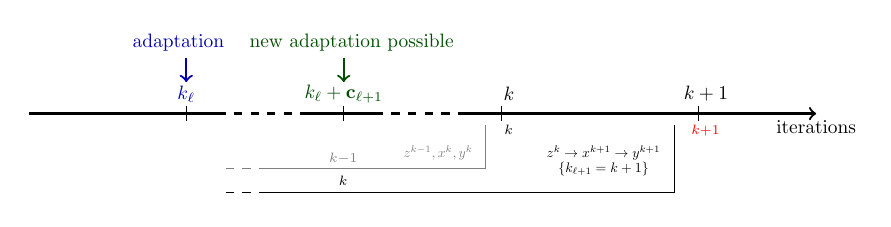
\begin{tikzpicture}
     %%% BASE
    \draw[thick, ->] (0,0) -- (10,0) node [below,scale=0.7] {iterations};
    \foreach \x in {1,...,3}
    \draw (2*\x, 0.1) -- node[pos=0.5] (point\x) {} (2*\x, -0.1);
    \draw (8.5, 0.1) -- node[pos=0.5] (point4) {} (8.5, -0.1);
    
    
     
          \draw[thick,dashed,white] (2.5,0) -- (3.5,0);
          \draw[thick,dashed,white] (4.5,0) -- (5.5,0);
    
    \node[scale=0.7] at (2,0.25) {\color{blue!70!black} $k_\ell$};
    

    \draw[thick,blue!70!black, ->] (2,0.7) -- (2,0.4) ;
    \node[scale = 0.7] at (1.9,0.9) {\color{blue!70!black} adaptation};
    
    

    
    
    
            %%% COord
            

    
   % \draw[thick,green!70!black, ->] (3,0.5) -- (3,0.1) ;
%    \node[scale = 0.7] at (3,0.7) {\color{green!70!black} coordination};
    
        \draw[thick,green!30!black, ->] (4,0.7) -- (4,0.4) ;
    \node[scale = 0.7] at (4,0.25) {\color{green!30!black} $k_\ell + \mathbf{c}_{\ell+1}$};
        \node[scale = 0.7] at (4.1,0.9) {\color{green!30!black} new adaptation possible};
    
    
    \node[scale = 0.5, gray] at (5.2,-0.5) { $z^{k-1},x^{k},y^{k}$};
    
    \node[scale = 0.7] at (6.1,0.25) { $k$};
    \node[scale = 0.7] at (6.1,-0.25) { $\Sel^k$};

    \draw[gray] (5.8,-0.15) -- (5.8,-0.7) -- (3,-0.7);
    \draw[dashed,gray] (2.5,-0.7) -- (3,-0.7);
    \node[scale = 0.7,gray] at (4,-0.6) { $\FF^{k-1}$};

    
    \node[scale = 0.5] at (7.3,-0.5) { $z^k\to x^{k+1} \to y^{k+1}$};
    \node[scale = 0.5] at (7.3,-0.7) { $\{ k_{\ell+1} = {k+1}\}$};
    
    \draw (8.2,-0.15) -- (8.2,-1.0) -- (3,-1.0);
    \draw[dashed] (2.5,-1.0) -- (3,-1.0);
    \node[scale = 0.7] at (4,-0.9) { $\FF^{k}$};
    
    
    \node[scale = 0.7] at (8.6,0.25) { $k+1$};
    \node[scale = 0.7,red] at (8.6,-0.25) { $\Sel^{k+1}$};



    
  %  \draw [very thick,green!70!black,->] (3,-0.1) to [out=-30,in=-150] (4.5,-0.1) ;
   %  \node[scale = 0.7] at (3.75,-0.5) {\color{green!70!black} $\leq T$};    
    
    %\draw [very thick,green!30!black,->] (4.5,-0.1) to [out=-30,in=-150] (6.5,-0.1) ;
    % \node[scale = 0.7] at (5.5,-0.5) {\color{green!30!black} $\leq T'$};
    
    
  \end{tikzpicture}}
  
  
      \caption{Summary of notations about iteration, adaptation and filtration. The filtration $\mathcal{F}^{k-1}$ is the sigma-algebra generated by $\{\Sel^\ell\}_{\ell\leq k-1}$ encompassing the knowledge of all variables up to $y^k$ (but not $z^k$).}
    \label{fig:proof}
  
  \end{figure}
}

\begin{proof}[Proof of Theorem \ref{th:conv_nondis_arbitrary}]
We start by noticing that, for a solution $x^\star$ of \eqref{eq:main_problem}, the proof of Theorem~\ref{th:conv_nondis} introduces the companion variable $z^\star =  \bQ\left(x^\star - \gamma\nabla f\left(x^\star\right)\right)$ which directly depends on $\bQ$, preventing us from a straightforward use of the results of Section\;\ref{sec:conv}. However, defining $z^{\star}_{\ell} =  \bQ_\ell\left(x^\star - \gamma\nabla f\left(x^\star\right)\right)$, Lemmas~\ref{lm:removing_exp} and \ref{lm:bub} can be directly extended and combined to show for any $k\in [k_\ell,k_{\ell+1})$ 
\begin{equation}\label{eq:iterate_flexible_lambda}
    \EE\left[\|z^{k} - z^{\star}_{\ell}\|_2^2\,|\,\FF^{k-1}\right] \leq \underbrace{  \left(1 -  \frac{2\gamma \mu L \lambda_{ \min}(\bP_\ell)}{\mu + L} \right) }_{\leq 1- \alpha_\ell} \|z^{k-1}-z^{\star}_{\ell}\|_2^2 .
\end{equation} 
%that for any $\gamma\in(0,2/(\mu+L)]$ and
Since the distribution of the selection has not changed since ${k}_{\ell}$, iterating \eqref{eq:iterate_flexible_lambda} leads to 
\begin{align}\label{eq:iterate_flexible_lambda2}
    \EE\left[\|z^{k} - z^{\star}_{\ell}\|_2^2\,|\,\FF^{k_{\ell}-1}\right] &\leq (1- \alpha_\ell)^{k-k_\ell} \|z^{k_\ell-1}-z^{\star}_{\ell}\|_2^2 .
\end{align}
We focus now on the term $\|z^{k_\ell-1}-z^{\star}_{\ell}\|_2^2$ corresponding to what happens at the last adaptation step. From the definition of variables in the algorithm and using the deterministic bound on $\|  \bQ_\ell   \bQ_{\ell-1}^{-1}\|$, we write
\begin{align}
  \nonumber  \EE\left[\|z^{k_\ell-1}-z^{\star}_{\ell}\|_2^2\,|\,\FF^{k_{\ell}-2}\right] &\leq   \EE\left[ \|  \bQ_\ell   \bQ_{\ell-1}^{-1}(z^{k_{\ell}-2} + P_{k_{\ell}-1}(y^{k_{\ell}-1}-z^{k_{\ell}-2}) - \bQ_\ell   \bQ_{\ell-1}^{-1}z^{\star}_{\ell-1}\|_2^2\,|\,\FF^{k_{\ell}-2}\right] \\[1.5ex]
        &\leq  \EE\left[ \|  \bQ_\ell   \bQ_{\ell-1}^{-1} \|_2^2   \|  z^{k_{\ell}-2} + P_{k_{\ell}-1}(y^{k_{\ell}-1}-z^{k_{\ell}-2}) - z^{\star}_{\ell-1}\|_2^2\,|\,\FF^{k_{\ell}-2}\right] \label{eq:Jadd} \\[1.5ex]
   \nonumber &\leq   \mathbf{a}_\ell  (1-\alpha_{\ell-1}) \|z^{k_\ell-2}-z^{\star}_{\ell-1}\|_2^2. \label{eq:adapt}
\end{align} 
Repeating this inequality backward to the previous adaptation step $z^{k_{\ell-1}}$, we get 
\begin{align}
  \nonumber  \EE\left[\|z^{k_\ell-1}-z^{\star}_{\ell}\|_2^2\,|\,\FF^{k_{\ell-1}}\right] &\leq  \mathbf{a}_\ell  (1-\alpha_{\ell-1})^{k_{\ell}-k_{\ell-1}} \|z^{k_{\ell-1}}-z^{\star}_{\ell-1}\|_2^2 \\
   &\leq  \mathbf{a}_\ell  (1-\alpha_{\ell-1})^{\mathbf{c}_\ell} \|z^{k_{\ell-1}}-z^{\star}_{\ell-1}\|_2^2,
\end{align} 
using the assumption of bounded inter-adaptation times.
Combining this inequality and \eqref{eq:iterate_flexible_lambda2}, we obtain that for any $k\in[k_\ell,k_{\ell+1})$, 
\begin{align*}
    \EE\left[\|z^{k}-z^{\star}_{\ell}\|_2^2\right] &\leq (1-\alpha_\ell)^{k-k_\ell}
    \prod_{m=1}^\ell  \mathbf{a}_m (1-\alpha_{m-1})^{\mathbf{c}_m} \|z^{0}-z^{\star}_{0}\|_2^2.
    \end{align*}
Using now \eqref{eq:corr-rate}, we get    
\[
\EE\left[\|z^{k}-z^{\star}_{\ell}\|_2^2\right] ~\leq~ (1-\alpha_\ell)^{k-k_\ell}
    \prod_{m=1}^\ell  (1-\beta_{m})^{\mathbf{c}_m} \|z^{0}-z^{\star}_{0}\|_2^2
    %~\leq~ (1-\alpha_\ell)^{k-k_\ell} (1-\beta)^{\sum_{m=1}^\ell \mathbf{c}_m}  \|z^{0}-z^{\star}_{0}\|_2^2.
\]
% \begin{align*}  
%   \EE\left[\|z^{k}-z^{\star}_{\ell}\|_2^2\right] &\leq (1-\alpha_\ell)^{k-k_\ell}
%     \prod_{m=1}^\ell  (1-\beta_{m})^{\mathbf{c}_m} \|z^{0}-z^{\star}_{0}\|_2^2\\
%     &\leq (1-\alpha_\ell)^{k-k_\ell} (1-\beta)^{\sum_{m=1}^\ell \mathbf{c}_m}  \|z^{0}-z^{\star}_{0}\|_2^2.
% \end{align*}
Finally, the non-expansiveness of the prox-operator propagates this inequality to $x_k$, since we have 
% $k\in(k_\ell,k_{\ell+1}]$ we have
\begin{align*}
\|x^k &- x^\star\|_2^2 = \|\prox_{\gamma g}(\bQ_\ell^{-1}(z^{k-1})) - \prox_{\gamma g}(\bQ_\ell^{-1}(z_\ell^\star))\|_2^2\\
&\leq
\|\bQ_\ell^{-1}(z^{k-1} - z_\ell^\star)\|_2^2 \leq \lambda_{\max}(\bQ_\ell^{-1})^2  \|z^{k-1}-z^\star_\ell\|_2^2 =  %\lambda_{\min}(\bP_\ell)  \|z^{k-1}-z^\star\|_2^2
\lambda_{\max}(\bP_\ell)  \|z^{k-1}-z^\star_\ell\|_2^2 \leq \|z^{k-1}-z^\star_\ell\|_2^2.
\end{align*}
This concludes the proof.
\end{proof}


\begin{example}[Explicit convergence rate] \label{ex:adapt_fixed}
Let us specify Theorem \eqref{th:conv_nondis_arbitrary} with the following simple adaptation strategy. We take a fixed upper bound on the adaptation cost and a fixed lower bound on uniformity:
\begin{equation}\label{eq:explicit}
\|  \bQ_\ell   \bQ_{\ell-1}^{-1} \|_2^2 \leq \mathbf{a} \qquad
\lambda_{ \min}(\bP_{\ell}) \geq \lambda.
\end{equation}
Then from the rate $1-\alpha = 1- 2\gamma\mu L\lambda/(\mu+L)$, we can perform an adaptation every 
\begin{align}
    \label{eq:min_adapt}
\mathbf{c} = \lceil \log(\mathbf{a})/\log\big((2-\alpha)/(2-2\alpha)\big)\rceil
\end{align}
 iterations, so that $\mathbf{a}(1-\alpha)^\mathbf{c} = (1-\alpha/2)^\mathbf{c}$ and $k_\ell = \ell \mathbf{c}$. A direct application of Theorem \eqref{th:conv_nondis_arbitrary} gives that, for any $k$,
 \begin{align*}
    \EE\left[\|x^{k+1}-x^{\star}_{\ell}\|_2^2\right] &\leq  \left(1-\frac{\gamma\mu L\lambda}{\mu+L}\right)^{k}  C
\end{align*}
where $C = \|z^0 - \bQ_0(x^\star - \gamma\nabla f(x^\star))\|_2^2$. That is the same convergence mode as in the non-adaptive case (Theorem\;\ref{th:conv_nondis}) with a modified rate. Note the modified rate provided here (of the form $(1-\alpha/2)$ to be compared with the $1-\alpha$ of Theorem\;\ref{th:conv_nondis}) was chosen for clarity; any rate strictly slower than $1-\alpha$ can bring the same result by adapting $\mathbf{c}$ accordingly.
\end{example}


% \begin{example}[Simpler result for coordinate projections] \label{ex:adapt_coord}
% The special case of subspace descent along coordinates (i.e.\;coordinate descent methods) leads to a simpler result. As discussed in Section~\ref{sec:coordproj}, the scaling matrices $(\bQ_\ell)$ commute with the proximity operator, so they can be removed from the algorithm. {Since no rescaling is needed in that case (line~\ref{line:rescale}, see Sec.~\ref{sec:coordproj}), there is no adaptation cost, $\mathbf{a}_{\ell} = 1$ for all $\ell$, and thus no inter-adaptation time, $\mathbf{c}_\ell = 1$ for all $\ell$, i.e. the sampling probabilites can be changed at every iteration. Then, under Assumptions \ref{hyp:f} and  \ref{hyp:main_identif}, the proof of the theorem simplifies and gives that for any $\gamma\in(0,2/(\mu+L)]$, we have for any $k\in [k_\ell,k_{\ell+1})$
% \begin{align*}
%     \EE\left[\|x^{k+1}-x^\star\|_2^2\right] &\leq C \left(1 -  \lambda_{\min}(\bP_{\ell})  \frac{2\gamma \mu L}{\mu + L}\right)^{k-k_\ell} \prod_{m=1}^\ell \left(1 -  \lambda_{\min}(\bP_{m-1})  \frac{2\gamma \mu L}{\mu + L}\right)^{k_m-k_{m-1}} \\
%     &= \mathcal{O}\left( \left(1 -  \lambda  \frac{2\gamma \mu L}{\mu + L}\right)^{k} \right)
% \end{align*}
% with $\lambda  = \lim\inf_\ell \lambda(\bP_\ell) >0$.}\hfill\Halmos
% \end{example}

{
\begin{remark}[On the adaptation frequency]
Theorem\;\ref{th:conv_nondis_arbitrary} and Example\;\ref{ex:adapt_fixed} tell us that we have to respect a prescribed number of iterations between two adaptation steps. We emphasize here that if this inter-adaptation time is violated, the resulting algorithm may be highly unstable. We illustrate this phenomenon on a TV-regularized least squares problem: we compare two versions of \adaalgo~with the same adaptation strategy verifying 
\eqref{eq:explicit} but with two different adaptation frequencies
\begin{itemize}
    \item at every iteration (i.e. taking $\mathbf{c}_\ell = 1$)
    \item following theory (i.e. taking $\mathbf{c}_\ell = \mathbf{c}$ as per Eq.~\eqref{eq:min_adapt})
\end{itemize}
On Figure~\ref{fig:stab}, we observe that adapting every iteration leads to chaotic behavior. Second, even though the theoretical number of iterations in an adaptation cycle is often pessimistic (due to the rough bounding of the rate), the iterates produced with this choice quickly become stable (i.e., identification happens, which will be shown and exploited in the next section) and show a steady decrease in suboptimality.

\begin{figure}[H]
\begin{center}
 \scalebox{0.9}{% This file was created by matplotlib2tikz v0.6.18.
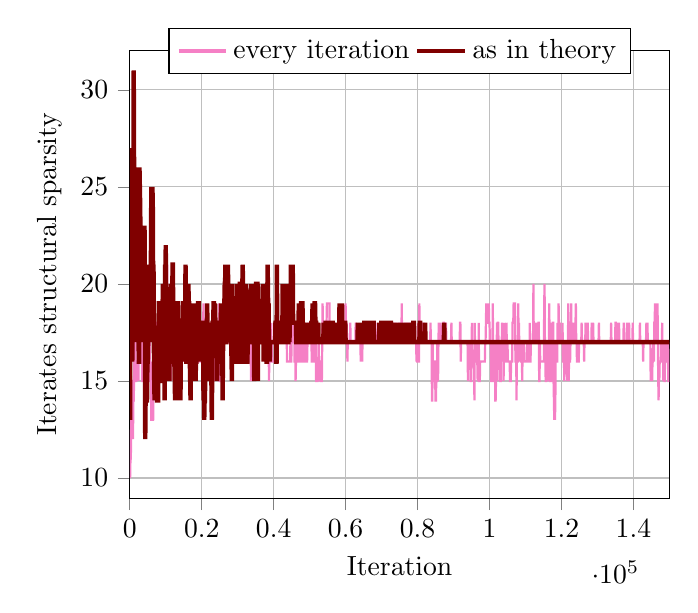
\begin{tikzpicture}


\begin{axis}[
legend cell align={left},
legend columns=2,
legend entries={{every iteration},{as in theory}},
legend style={at={(0.5,1.05)}, anchor=north},
tick align=outside,
tick pos=left,
xlabel={Iteration},
xmajorgrids,
xmin=0, xmax=150000,
ylabel={Iterates structural sparsity},
ymajorgrids,
ymin=8.95, ymax=32.05
]
\addlegendimage{no markers, very thick , magenta!50!white}
\addlegendimage{no markers, ultra thick, red!50!black}
\addplot [ thick, magenta!50!white]
table [row sep=\\]{%
0	11 \\
100	10 \\
200	11 \\
300	11 \\
400	13 \\
500	15 \\
600	15 \\
700	15 \\
800	14 \\
900	12 \\
1000	14 \\
1100	14 \\
1200	15 \\
1300	18 \\
1400	19 \\
1500	15 \\
1600	15 \\
1700	15 \\
1800	15 \\
1900	16 \\
2000	16 \\
2100	16 \\
2200	16 \\
2300	18 \\
2400	15 \\
2500	17 \\
2600	17 \\
2700	16 \\
2800	17 \\
2900	18 \\
3000	16 \\
3100	16 \\
3200	16 \\
3300	20 \\
3400	15 \\
3500	15 \\
3600	16 \\
3700	16 \\
3800	16 \\
3900	17 \\
4000	17 \\
4100	18 \\
4200	18 \\
4300	18 \\
4400	17 \\
4500	17 \\
4600	15 \\
4700	15 \\
4800	15 \\
4900	15 \\
5000	16 \\
5100	16 \\
5200	15 \\
5300	15 \\
5400	15 \\
5500	18 \\
5600	16 \\
5700	15 \\
5800	15 \\
5900	16 \\
6000	13 \\
6100	13 \\
6200	15 \\
6300	15 \\
6400	13 \\
6500	13 \\
6600	15 \\
6700	16 \\
6800	16 \\
6900	18 \\
7000	16 \\
7100	16 \\
7200	16 \\
7300	17 \\
7400	17 \\
7500	18 \\
7600	18 \\
7700	16 \\
7800	16 \\
7900	16 \\
8000	16 \\
8100	15 \\
8200	15 \\
8300	17 \\
8400	17 \\
8500	16 \\
8600	15 \\
8700	15 \\
8800	17 \\
8900	16 \\
9000	16 \\
9100	17 \\
9200	17 \\
9300	20 \\
9400	18 \\
9500	17 \\
9600	17 \\
9700	15 \\
9800	15 \\
9900	17 \\
10000	17 \\
10100	18 \\
10200	17 \\
10300	17 \\
10400	21 \\
10500	16 \\
10600	16 \\
10700	16 \\
10800	16 \\
10900	16 \\
11000	16 \\
11100	16 \\
11200	16 \\
11300	16 \\
11400	15 \\
11500	16 \\
11600	16 \\
11700	17 \\
11800	17 \\
11900	16 \\
12000	16 \\
12100	17 \\
12200	16 \\
12300	17 \\
12400	16 \\
12500	17 \\
12600	18 \\
12700	17 \\
12800	17 \\
12900	16 \\
13000	16 \\
13100	17 \\
13200	16 \\
13300	17 \\
13400	18 \\
13500	16 \\
13600	16 \\
13700	17 \\
13800	15 \\
13900	16 \\
14000	16 \\
14100	16 \\
14200	16 \\
14300	17 \\
14400	17 \\
14500	16 \\
14600	18 \\
14700	16 \\
14800	17 \\
14900	18 \\
15000	18 \\
15100	17 \\
15200	17 \\
15300	17 \\
15400	17 \\
15500	17 \\
15600	18 \\
15700	17 \\
15800	17 \\
15900	17 \\
16000	17 \\
16100	17 \\
16200	17 \\
16300	17 \\
16400	17 \\
16500	17 \\
16600	17 \\
16700	19 \\
16800	18 \\
16900	17 \\
17000	17 \\
17100	17 \\
17200	17 \\
17300	18 \\
17400	16 \\
17500	16 \\
17600	16 \\
17700	16 \\
17800	17 \\
17900	16 \\
18000	16 \\
18100	16 \\
18200	16 \\
18300	17 \\
18400	17 \\
18500	18 \\
18600	17 \\
18700	18 \\
18800	17 \\
18900	17 \\
19000	17 \\
19100	17 \\
19200	17 \\
19300	16 \\
19400	16 \\
19500	16 \\
19600	17 \\
19700	17 \\
19800	17 \\
19900	17 \\
20000	17 \\
20100	17 \\
20200	17 \\
20300	18 \\
20400	18 \\
20500	19 \\
20600	17 \\
20700	17 \\
20800	17 \\
20900	17 \\
21000	15 \\
21100	17 \\
21200	17 \\
21300	18 \\
21400	17 \\
21500	17 \\
21600	17 \\
21700	16 \\
21800	16 \\
21900	17 \\
22000	16 \\
22100	16 \\
22200	16 \\
22300	17 \\
22400	16 \\
22500	17 \\
22600	16 \\
22700	15 \\
22800	16 \\
22900	16 \\
23000	16 \\
23100	16 \\
23200	16 \\
23300	16 \\
23400	17 \\
23500	17 \\
23600	15 \\
23700	17 \\
23800	16 \\
23900	16 \\
24000	16 \\
24100	16 \\
24200	16 \\
24300	16 \\
24400	16 \\
24500	15 \\
24600	18 \\
24700	16 \\
24800	19 \\
24900	18 \\
25000	15 \\
25100	15 \\
25200	15 \\
25300	16 \\
25400	17 \\
25500	16 \\
25600	16 \\
25700	17 \\
25800	17 \\
25900	17 \\
26000	18 \\
26100	17 \\
26200	17 \\
26300	17 \\
26400	17 \\
26500	17 \\
26600	18 \\
26700	17 \\
26800	17 \\
26900	17 \\
27000	18 \\
27100	17 \\
27200	17 \\
27300	17 \\
27400	18 \\
27500	17 \\
27600	17 \\
27700	17 \\
27800	17 \\
27900	17 \\
28000	17 \\
28100	17 \\
28200	18 \\
28300	18 \\
28400	17 \\
28500	17 \\
28600	17 \\
28700	17 \\
28800	17 \\
28900	18 \\
29000	17 \\
29100	17 \\
29200	17 \\
29300	17 \\
29400	17 \\
29500	17 \\
29600	17 \\
29700	17 \\
29800	17 \\
29900	17 \\
30000	17 \\
30100	17 \\
30200	17 \\
30300	17 \\
30400	17 \\
30500	18 \\
30600	17 \\
30700	17 \\
30800	17 \\
30900	18 \\
31000	17 \\
31100	17 \\
31200	17 \\
31300	17 \\
31400	17 \\
31500	17 \\
31600	17 \\
31700	17 \\
31800	17 \\
31900	17 \\
32000	17 \\
32100	17 \\
32200	17 \\
32300	17 \\
32400	17 \\
32500	17 \\
32600	17 \\
32700	18 \\
32800	17 \\
32900	17 \\
33000	17 \\
33100	17 \\
33200	16 \\
33300	16 \\
33400	18 \\
33500	16 \\
33600	17 \\
33700	15 \\
33800	16 \\
33900	18 \\
34000	16 \\
34100	16 \\
34200	15 \\
34300	17 \\
34400	17 \\
34500	16 \\
34600	16 \\
34700	16 \\
34800	17 \\
34900	17 \\
35000	17 \\
35100	17 \\
35200	17 \\
35300	18 \\
35400	17 \\
35500	18 \\
35600	17 \\
35700	17 \\
35800	17 \\
35900	17 \\
36000	17 \\
36100	17 \\
36200	17 \\
36300	17 \\
36400	17 \\
36500	17 \\
36600	17 \\
36700	17 \\
36800	17 \\
36900	17 \\
37000	17 \\
37100	17 \\
37200	18 \\
37300	17 \\
37400	17 \\
37500	17 \\
37600	17 \\
37700	17 \\
37800	17 \\
37900	18 \\
38000	17 \\
38100	17 \\
38200	17 \\
38300	18 \\
38400	17 \\
38500	18 \\
38600	17 \\
38700	15 \\
38800	16 \\
38900	16 \\
39000	16 \\
39100	16 \\
39200	16 \\
39300	18 \\
39400	16 \\
39500	17 \\
39600	16 \\
39700	16 \\
39800	16 \\
39900	16 \\
40000	16 \\
40100	16 \\
40200	16 \\
40300	16 \\
40400	16 \\
40500	17 \\
40600	17 \\
40700	16 \\
40800	16 \\
40900	17 \\
41000	17 \\
41100	17 \\
41200	17 \\
41300	17 \\
41400	17 \\
41500	17 \\
41600	17 \\
41700	17 \\
41800	17 \\
41900	17 \\
42000	18 \\
42100	17 \\
42200	17 \\
42300	18 \\
42400	18 \\
42500	17 \\
42600	17 \\
42700	17 \\
42800	17 \\
42900	17 \\
43000	17 \\
43100	17 \\
43200	17 \\
43300	18 \\
43400	18 \\
43500	17 \\
43600	18 \\
43700	16 \\
43800	16 \\
43900	16 \\
44000	16 \\
44100	16 \\
44200	16 \\
44300	16 \\
44400	16 \\
44500	16 \\
44600	16 \\
44700	18 \\
44800	16 \\
44900	16 \\
45000	17 \\
45100	17 \\
45200	17 \\
45300	17 \\
45400	19 \\
45500	17 \\
45600	17 \\
45700	18 \\
45800	16 \\
45900	16 \\
46000	17 \\
46100	15 \\
46200	16 \\
46300	16 \\
46400	16 \\
46500	16 \\
46600	16 \\
46700	18 \\
46800	16 \\
46900	16 \\
47000	16 \\
47100	16 \\
47200	18 \\
47300	16 \\
47400	16 \\
47500	18 \\
47600	16 \\
47700	16 \\
47800	16 \\
47900	16 \\
48000	16 \\
48100	17 \\
48200	17 \\
48300	17 \\
48400	18 \\
48500	16 \\
48600	16 \\
48700	16 \\
48800	16 \\
48900	16 \\
49000	16 \\
49100	17 \\
49200	16 \\
49300	16 \\
49400	17 \\
49500	18 \\
49600	17 \\
49700	17 \\
49800	17 \\
49900	17 \\
50000	17 \\
50100	17 \\
50200	17 \\
50300	17 \\
50400	17 \\
50500	17 \\
50600	16 \\
50700	16 \\
50800	16 \\
50900	16 \\
51000	17 \\
51100	16 \\
51200	16 \\
51300	16 \\
51400	18 \\
51500	16 \\
51600	16 \\
51700	17 \\
51800	15 \\
51900	15 \\
52000	15 \\
52100	15 \\
52200	15 \\
52300	16 \\
52400	15 \\
52500	17 \\
52600	16 \\
52700	16 \\
52800	16 \\
52900	16 \\
53000	16 \\
53100	15 \\
53200	15 \\
53300	15 \\
53400	15 \\
53500	17 \\
53600	19 \\
53700	18 \\
53800	18 \\
53900	18 \\
54000	18 \\
54100	18 \\
54200	18 \\
54300	18 \\
54400	18 \\
54500	18 \\
54600	18 \\
54700	18 \\
54800	19 \\
54900	19 \\
55000	19 \\
55100	19 \\
55200	19 \\
55300	19 \\
55400	19 \\
55500	19 \\
55600	17 \\
55700	18 \\
55800	17 \\
55900	17 \\
56000	17 \\
56100	17 \\
56200	17 \\
56300	17 \\
56400	18 \\
56500	18 \\
56600	17 \\
56700	17 \\
56800	17 \\
56900	17 \\
57000	18 \\
57100	17 \\
57200	17 \\
57300	17 \\
57400	17 \\
57500	17 \\
57600	17 \\
57700	17 \\
57800	17 \\
57900	17 \\
58000	17 \\
58100	17 \\
58200	17 \\
58300	17 \\
58400	17 \\
58500	17 \\
58600	17 \\
58700	17 \\
58800	17 \\
58900	17 \\
59000	17 \\
59100	18 \\
59200	18 \\
59300	17 \\
59400	17 \\
59500	17 \\
59600	17 \\
59700	18 \\
59800	17 \\
59900	17 \\
60000	19 \\
60100	17 \\
60200	17 \\
60300	18 \\
60400	17 \\
60500	16 \\
60600	17 \\
60700	17 \\
60800	17 \\
60900	17 \\
61000	17 \\
61100	17 \\
61200	17 \\
61300	18 \\
61400	17 \\
61500	17 \\
61600	17 \\
61700	17 \\
61800	17 \\
61900	17 \\
62000	17 \\
62100	17 \\
62200	17 \\
62300	17 \\
62400	17 \\
62500	17 \\
62600	17 \\
62700	17 \\
62800	18 \\
62900	17 \\
63000	17 \\
63100	17 \\
63200	17 \\
63300	17 \\
63400	17 \\
63500	17 \\
63600	17 \\
63700	17 \\
63800	17 \\
63900	17 \\
64000	17 \\
64100	17 \\
64200	16 \\
64300	17 \\
64400	16 \\
64500	17 \\
64600	16 \\
64700	17 \\
64800	17 \\
64900	18 \\
65000	17 \\
65100	17 \\
65200	18 \\
65300	17 \\
65400	17 \\
65500	17 \\
65600	17 \\
65700	17 \\
65800	17 \\
65900	17 \\
66000	17 \\
66100	17 \\
66200	17 \\
66300	17 \\
66400	17 \\
66500	17 \\
66600	17 \\
66700	17 \\
66800	17 \\
66900	17 \\
67000	18 \\
67100	17 \\
67200	17 \\
67300	17 \\
67400	17 \\
67500	17 \\
67600	17 \\
67700	17 \\
67800	17 \\
67900	17 \\
68000	17 \\
68100	18 \\
68200	17 \\
68300	18 \\
68400	17 \\
68500	17 \\
68600	17 \\
68700	17 \\
68800	17 \\
68900	17 \\
69000	17 \\
69100	17 \\
69200	17 \\
69300	17 \\
69400	17 \\
69500	17 \\
69600	18 \\
69700	17 \\
69800	18 \\
69900	17 \\
70000	17 \\
70100	17 \\
70200	17 \\
70300	17 \\
70400	17 \\
70500	17 \\
70600	17 \\
70700	17 \\
70800	17 \\
70900	17 \\
71000	17 \\
71100	17 \\
71200	17 \\
71300	17 \\
71400	17 \\
71500	17 \\
71600	17 \\
71700	17 \\
71800	17 \\
71900	17 \\
72000	17 \\
72100	17 \\
72200	17 \\
72300	17 \\
72400	17 \\
72500	17 \\
72600	17 \\
72700	17 \\
72800	17 \\
72900	17 \\
73000	17 \\
73100	17 \\
73200	18 \\
73300	17 \\
73400	17 \\
73500	17 \\
73600	18 \\
73700	17 \\
73800	17 \\
73900	18 \\
74000	17 \\
74100	17 \\
74200	17 \\
74300	17 \\
74400	17 \\
74500	17 \\
74600	17 \\
74700	17 \\
74800	18 \\
74900	17 \\
75000	17 \\
75100	17 \\
75200	17 \\
75300	18 \\
75400	17 \\
75500	17 \\
75600	19 \\
75700	17 \\
75800	17 \\
75900	17 \\
76000	17 \\
76100	17 \\
76200	17 \\
76300	17 \\
76400	17 \\
76500	18 \\
76600	17 \\
76700	17 \\
76800	17 \\
76900	17 \\
77000	18 \\
77100	17 \\
77200	17 \\
77300	17 \\
77400	17 \\
77500	17 \\
77600	18 \\
77700	17 \\
77800	18 \\
77900	17 \\
78000	17 \\
78100	17 \\
78200	17 \\
78300	17 \\
78400	17 \\
78500	17 \\
78600	17 \\
78700	18 \\
78800	17 \\
78900	17 \\
79000	18 \\
79100	17 \\
79200	17 \\
79300	17 \\
79400	17 \\
79500	17 \\
79600	17 \\
79700	16 \\
79800	17 \\
79900	16 \\
80000	16 \\
80100	18 \\
80200	16 \\
80300	16 \\
80400	16 \\
80500	19 \\
80600	17 \\
80700	18 \\
80800	17 \\
80900	18 \\
81000	17 \\
81100	17 \\
81200	17 \\
81300	17 \\
81400	17 \\
81500	17 \\
81600	18 \\
81700	17 \\
81800	18 \\
81900	17 \\
82000	17 \\
82100	17 \\
82200	17 \\
82300	17 \\
82400	17 \\
82500	17 \\
82600	17 \\
82700	17 \\
82800	17 \\
82900	17 \\
83000	17 \\
83100	17 \\
83200	17 \\
83300	17 \\
83400	17 \\
83500	17 \\
83600	18 \\
83700	17 \\
83800	17 \\
83900	17 \\
84000	14 \\
84100	14 \\
84200	17 \\
84300	15 \\
84400	15 \\
84500	15 \\
84600	16 \\
84700	16 \\
84800	16 \\
84900	15 \\
85000	14 \\
85100	14 \\
85200	15 \\
85300	15 \\
85400	15 \\
85500	17 \\
85600	16 \\
85700	15 \\
85800	17 \\
85900	18 \\
86000	17 \\
86100	17 \\
86200	17 \\
86300	17 \\
86400	18 \\
86500	17 \\
86600	17 \\
86700	17 \\
86800	17 \\
86900	17 \\
87000	17 \\
87100	17 \\
87200	18 \\
87300	18 \\
87400	17 \\
87500	18 \\
87600	17 \\
87700	17 \\
87800	17 \\
87900	18 \\
88000	17 \\
88100	17 \\
88200	17 \\
88300	17 \\
88400	17 \\
88500	17 \\
88600	17 \\
88700	17 \\
88800	17 \\
88900	17 \\
89000	17 \\
89100	17 \\
89200	17 \\
89300	17 \\
89400	18 \\
89500	17 \\
89600	17 \\
89700	17 \\
89800	17 \\
89900	17 \\
90000	17 \\
90100	17 \\
90200	17 \\
90300	17 \\
90400	17 \\
90500	17 \\
90600	17 \\
90700	17 \\
90800	17 \\
90900	17 \\
91000	17 \\
91100	17 \\
91200	17 \\
91300	17 \\
91400	17 \\
91500	17 \\
91600	17 \\
91700	17 \\
91800	18 \\
91900	18 \\
92000	16 \\
92100	17 \\
92200	17 \\
92300	17 \\
92400	17 \\
92500	17 \\
92600	17 \\
92700	17 \\
92800	17 \\
92900	17 \\
93000	17 \\
93100	17 \\
93200	17 \\
93300	17 \\
93400	17 \\
93500	17 \\
93600	17 \\
93700	17 \\
93800	17 \\
93900	17 \\
94000	15 \\
94100	16 \\
94200	16 \\
94300	16 \\
94400	16 \\
94500	17 \\
94600	16 \\
94700	17 \\
94800	15 \\
94900	15 \\
95000	16 \\
95100	18 \\
95200	16 \\
95300	16 \\
95400	16 \\
95500	16 \\
95600	16 \\
95700	16 \\
95800	14 \\
95900	18 \\
96000	16 \\
96100	16 \\
96200	17 \\
96300	16 \\
96400	16 \\
96500	17 \\
96600	16 \\
96700	15 \\
96800	17 \\
96900	15 \\
97000	18 \\
97100	15 \\
97200	15 \\
97300	15 \\
97400	16 \\
97500	16 \\
97600	16 \\
97700	16 \\
97800	16 \\
97900	16 \\
98000	16 \\
98100	16 \\
98200	16 \\
98300	16 \\
98400	16 \\
98500	16 \\
98600	16 \\
98700	16 \\
98800	17 \\
98900	17 \\
99000	18 \\
99100	19 \\
99200	18 \\
99300	18 \\
99400	18 \\
99500	18 \\
99600	18 \\
99700	18 \\
99800	19 \\
99900	18 \\
100000	18 \\
100100	17 \\
100200	17 \\
100300	17 \\
100400	17 \\
100500	15 \\
100600	15 \\
100700	16 \\
100800	16 \\
100900	19 \\
101000	17 \\
101100	17 \\
101200	17 \\
101300	15 \\
101400	15 \\
101500	16 \\
101600	14 \\
101700	14 \\
101800	15 \\
101900	17 \\
102000	17 \\
102100	18 \\
102200	15 \\
102300	18 \\
102400	18 \\
102500	17 \\
102600	17 \\
102700	16 \\
102800	16 \\
102900	16 \\
103000	15 \\
103100	15 \\
103200	17 \\
103300	16 \\
103400	17 \\
103500	18 \\
103600	17 \\
103700	17 \\
103800	18 \\
103900	15 \\
104000	16 \\
104100	16 \\
104200	18 \\
104300	17 \\
104400	16 \\
104500	16 \\
104600	16 \\
104700	18 \\
104800	17 \\
104900	17 \\
105000	17 \\
105100	16 \\
105200	16 \\
105300	16 \\
105400	16 \\
105500	16 \\
105600	16 \\
105700	15 \\
105800	15 \\
105900	15 \\
106000	16 \\
106100	16 \\
106200	16 \\
106300	16 \\
106400	18 \\
106500	18 \\
106600	18 \\
106700	19 \\
106800	19 \\
106900	19 \\
107000	19 \\
107100	19 \\
107200	16 \\
107300	16 \\
107400	17 \\
107500	14 \\
107600	16 \\
107700	16 \\
107800	16 \\
107900	16 \\
108000	19 \\
108100	16 \\
108200	18 \\
108300	16 \\
108400	17 \\
108500	16 \\
108600	17 \\
108700	17 \\
108800	16 \\
108900	16 \\
109000	16 \\
109100	15 \\
109200	17 \\
109300	17 \\
109400	17 \\
109500	17 \\
109600	17 \\
109700	16 \\
109800	16 \\
109900	16 \\
110000	16 \\
110100	16 \\
110200	16 \\
110300	16 \\
110400	16 \\
110500	17 \\
110600	17 \\
110700	17 \\
110800	17 \\
110900	16 \\
111000	16 \\
111100	16 \\
111200	18 \\
111300	16 \\
111400	16 \\
111500	17 \\
111600	17 \\
111700	17 \\
111800	17 \\
111900	17 \\
112000	17 \\
112100	17 \\
112200	20 \\
112300	17 \\
112400	17 \\
112500	17 \\
112600	17 \\
112700	17 \\
112800	17 \\
112900	18 \\
113000	17 \\
113100	17 \\
113200	17 \\
113300	17 \\
113400	18 \\
113500	17 \\
113600	18 \\
113700	18 \\
113800	15 \\
113900	15 \\
114000	17 \\
114100	16 \\
114200	16 \\
114300	16 \\
114400	16 \\
114500	16 \\
114600	16 \\
114700	16 \\
114800	16 \\
114900	16 \\
115000	16 \\
115100	16 \\
115200	19 \\
115300	20 \\
115400	17 \\
115500	17 \\
115600	15 \\
115700	15 \\
115800	15 \\
115900	17 \\
116000	16 \\
116100	16 \\
116200	17 \\
116300	16 \\
116400	15 \\
116500	17 \\
116600	19 \\
116700	17 \\
116800	15 \\
116900	15 \\
117000	15 \\
117100	17 \\
117200	18 \\
117300	15 \\
117400	16 \\
117500	16 \\
117600	18 \\
117700	18 \\
117800	15 \\
117900	14 \\
118000	13 \\
118100	15 \\
118200	13 \\
118300	14 \\
118400	17 \\
118500	16 \\
118600	16 \\
118700	16 \\
118800	16 \\
118900	18 \\
119000	17 \\
119100	17 \\
119200	19 \\
119300	18 \\
119400	17 \\
119500	18 \\
119600	17 \\
119700	17 \\
119800	17 \\
119900	17 \\
120000	17 \\
120100	17 \\
120200	17 \\
120300	18 \\
120400	16 \\
120500	16 \\
120600	16 \\
120700	16 \\
120800	15 \\
120900	17 \\
121000	16 \\
121100	16 \\
121200	17 \\
121300	16 \\
121400	16 \\
121500	16 \\
121600	15 \\
121700	17 \\
121800	17 \\
121900	19 \\
122000	15 \\
122100	16 \\
122200	16 \\
122300	16 \\
122400	16 \\
122500	17 \\
122600	17 \\
122700	19 \\
122800	17 \\
122900	17 \\
123000	17 \\
123100	17 \\
123200	17 \\
123300	17 \\
123400	18 \\
123500	17 \\
123600	17 \\
123700	17 \\
123800	17 \\
123900	18 \\
124000	19 \\
124100	17 \\
124200	17 \\
124300	16 \\
124400	16 \\
124500	16 \\
124600	16 \\
124700	16 \\
124800	16 \\
124900	17 \\
125000	17 \\
125100	17 \\
125200	17 \\
125300	17 \\
125400	17 \\
125500	17 \\
125600	18 \\
125700	17 \\
125800	17 \\
125900	17 \\
126000	17 \\
126100	17 \\
126200	17 \\
126300	16 \\
126400	17 \\
126500	17 \\
126600	17 \\
126700	18 \\
126800	17 \\
126900	17 \\
127000	17 \\
127100	17 \\
127200	17 \\
127300	18 \\
127400	17 \\
127500	17 \\
127600	17 \\
127700	17 \\
127800	17 \\
127900	17 \\
128000	17 \\
128100	17 \\
128200	17 \\
128300	17 \\
128400	18 \\
128500	17 \\
128600	17 \\
128700	17 \\
128800	18 \\
128900	17 \\
129000	17 \\
129100	17 \\
129200	17 \\
129300	17 \\
129400	17 \\
129500	17 \\
129600	17 \\
129700	17 \\
129800	17 \\
129900	17 \\
130000	17 \\
130100	17 \\
130200	17 \\
130300	17 \\
130400	18 \\
130500	17 \\
130600	17 \\
130700	17 \\
130800	17 \\
130900	17 \\
131000	17 \\
131100	17 \\
131200	17 \\
131300	17 \\
131400	17 \\
131500	17 \\
131600	17 \\
131700	17 \\
131800	17 \\
131900	17 \\
132000	17 \\
132100	17 \\
132200	17 \\
132300	17 \\
132400	17 \\
132500	17 \\
132600	17 \\
132700	17 \\
132800	17 \\
132900	17 \\
133000	17 \\
133100	17 \\
133200	17 \\
133300	17 \\
133400	17 \\
133500	17 \\
133600	17 \\
133700	17 \\
133800	18 \\
133900	17 \\
134000	17 \\
134100	17 \\
134200	17 \\
134300	17 \\
134400	17 \\
134500	17 \\
134600	17 \\
134700	17 \\
134800	17 \\
134900	17 \\
135000	18 \\
135100	18 \\
135200	17 \\
135300	17 \\
135400	17 \\
135500	17 \\
135600	17 \\
135700	18 \\
135800	17 \\
135900	17 \\
136000	18 \\
136100	17 \\
136200	17 \\
136300	17 \\
136400	17 \\
136500	17 \\
136600	17 \\
136700	17 \\
136800	17 \\
136900	17 \\
137000	17 \\
137100	17 \\
137200	17 \\
137300	18 \\
137400	17 \\
137500	17 \\
137600	17 \\
137700	17 \\
137800	17 \\
137900	17 \\
138000	17 \\
138100	17 \\
138200	18 \\
138300	17 \\
138400	17 \\
138500	18 \\
138600	17 \\
138700	17 \\
138800	18 \\
138900	17 \\
139000	17 \\
139100	17 \\
139200	17 \\
139300	17 \\
139400	17 \\
139500	17 \\
139600	17 \\
139700	17 \\
139800	18 \\
139900	17 \\
140000	17 \\
140100	17 \\
140200	17 \\
140300	17 \\
140400	17 \\
140500	17 \\
140600	17 \\
140700	17 \\
140800	17 \\
140900	17 \\
141000	17 \\
141100	17 \\
141200	17 \\
141300	17 \\
141400	17 \\
141500	17 \\
141600	17 \\
141700	17 \\
141800	18 \\
141900	17 \\
142000	17 \\
142100	17 \\
142200	17 \\
142300	17 \\
142400	17 \\
142500	17 \\
142600	17 \\
142700	16 \\
142800	17 \\
142900	17 \\
143000	17 \\
143100	17 \\
143200	17 \\
143300	17 \\
143400	17 \\
143500	17 \\
143600	18 \\
143700	17 \\
143800	17 \\
143900	18 \\
144000	17 \\
144100	17 \\
144200	17 \\
144300	17 \\
144400	17 \\
144500	17 \\
144600	17 \\
144700	17 \\
144800	15 \\
144900	16 \\
145000	16 \\
145100	16 \\
145200	15 \\
145300	16 \\
145400	16 \\
145500	17 \\
145600	17 \\
145700	16 \\
145800	18 \\
145900	18 \\
146000	19 \\
146100	18 \\
146200	17 \\
146300	17 \\
146400	19 \\
146500	17 \\
146600	18 \\
146700	19 \\
146800	17 \\
146900	15 \\
147000	14 \\
147100	16 \\
147200	15 \\
147300	16 \\
147400	16 \\
147500	16 \\
147600	16 \\
147700	17 \\
147800	17 \\
147900	17 \\
148000	18 \\
148100	16 \\
148200	17 \\
148300	15 \\
148400	16 \\
148500	17 \\
148600	15 \\
148700	15 \\
148800	17 \\
148900	16 \\
149000	16 \\
149100	16 \\
149200	16 \\
149300	17 \\
149400	17 \\
149500	17 \\
149600	16 \\
149700	15 \\
149800	15 \\
149900	15 \\
150000	16 \\
150100	16 \\
150200	16 \\
150300	17 \\
150400	16 \\
150500	17 \\
150600	17 \\
150700	16 \\
150800	16 \\
150900	17 \\
151000	15 \\
151100	16 \\
151200	17 \\
151300	17 \\
151400	15 \\
151500	16 \\
151600	16 \\
151700	17 \\
151800	16 \\
151900	16 \\
152000	16 \\
152100	15 \\
152200	16 \\
152300	17 \\
152400	16 \\
152500	16 \\
152600	15 \\
152700	18 \\
152800	17 \\
152900	17 \\
153000	16 \\
153100	16 \\
153200	16 \\
153300	16 \\
153400	16 \\
153500	16 \\
153600	17 \\
153700	17 \\
153800	17 \\
153900	17 \\
154000	17 \\
154100	17 \\
154200	18 \\
154300	17 \\
154400	18 \\
154500	18 \\
154600	17 \\
154700	17 \\
154800	17 \\
154900	18 \\
155000	16 \\
155100	16 \\
155200	17 \\
155300	17 \\
155400	17 \\
155500	17 \\
155600	17 \\
155700	17 \\
155800	17 \\
155900	18 \\
156000	18 \\
156100	17 \\
156200	18 \\
156300	17 \\
156400	17 \\
156500	17 \\
156600	17 \\
156700	17 \\
156800	17 \\
156900	17 \\
157000	17 \\
157100	17 \\
157200	17 \\
157300	17 \\
157400	17 \\
157500	17 \\
157600	18 \\
157700	17 \\
157800	17 \\
157900	17 \\
158000	18 \\
158100	17 \\
158200	17 \\
158300	17 \\
158400	17 \\
158500	17 \\
158600	17 \\
158700	17 \\
158800	17 \\
158900	17 \\
159000	17 \\
159100	17 \\
159200	17 \\
159300	17 \\
159400	17 \\
159500	17 \\
159600	17 \\
159700	17 \\
159800	17 \\
159900	17 \\
160000	17 \\
160100	17 \\
160200	17 \\
160300	17 \\
160400	17 \\
160500	17 \\
160600	17 \\
160700	17 \\
160800	17 \\
160900	17 \\
161000	17 \\
161100	18 \\
161200	17 \\
161300	17 \\
161400	17 \\
161500	17 \\
161600	17 \\
161700	17 \\
161800	17 \\
161900	17 \\
162000	17 \\
162100	17 \\
162200	17 \\
162300	17 \\
162400	17 \\
162500	17 \\
162600	17 \\
162700	17 \\
162800	17 \\
162900	18 \\
163000	17 \\
163100	19 \\
163200	17 \\
163300	17 \\
163400	17 \\
163500	17 \\
163600	17 \\
163700	18 \\
163800	17 \\
163900	17 \\
164000	17 \\
164100	17 \\
164200	17 \\
164300	17 \\
164400	17 \\
164500	17 \\
164600	17 \\
164700	17 \\
164800	17 \\
164900	18 \\
165000	17 \\
165100	17 \\
165200	18 \\
165300	17 \\
165400	18 \\
165500	18 \\
165600	17 \\
165700	17 \\
165800	17 \\
165900	17 \\
166000	17 \\
166100	17 \\
166200	17 \\
166300	17 \\
166400	17 \\
166500	17 \\
166600	17 \\
166700	17 \\
166800	15 \\
166900	15 \\
167000	17 \\
167100	18 \\
167200	17 \\
167300	17 \\
167400	17 \\
167500	17 \\
167600	17 \\
167700	19 \\
167800	17 \\
167900	17 \\
168000	17 \\
168100	17 \\
168200	17 \\
168300	17 \\
168400	17 \\
168500	17 \\
168600	17 \\
168700	17 \\
168800	17 \\
168900	17 \\
169000	18 \\
169100	17 \\
169200	18 \\
169300	18 \\
169400	17 \\
169500	17 \\
169600	19 \\
169700	17 \\
169800	17 \\
169900	15 \\
170000	15 \\
170100	16 \\
170200	19 \\
170300	17 \\
170400	17 \\
170500	17 \\
170600	17 \\
170700	17 \\
170800	16 \\
170900	15 \\
171000	16 \\
171100	16 \\
171200	16 \\
171300	16 \\
171400	13 \\
171500	17 \\
171600	18 \\
171700	17 \\
171800	17 \\
171900	19 \\
172000	17 \\
172100	17 \\
172200	17 \\
172300	17 \\
172400	17 \\
172500	17 \\
172600	17 \\
172700	17 \\
172800	17 \\
172900	17 \\
173000	17 \\
173100	17 \\
173200	17 \\
173300	17 \\
173400	17 \\
173500	17 \\
173600	17 \\
173700	17 \\
173800	18 \\
173900	17 \\
174000	17 \\
174100	17 \\
174200	17 \\
174300	17 \\
174400	17 \\
174500	17 \\
174600	17 \\
174700	17 \\
174800	17 \\
174900	17 \\
175000	17 \\
175100	17 \\
175200	17 \\
175300	17 \\
175400	17 \\
175500	17 \\
175600	17 \\
175700	17 \\
175800	18 \\
175900	17 \\
176000	17 \\
176100	17 \\
176200	18 \\
176300	17 \\
176400	17 \\
176500	17 \\
176600	18 \\
176700	17 \\
176800	17 \\
176900	17 \\
177000	17 \\
177100	17 \\
177200	17 \\
177300	17 \\
177400	18 \\
177500	17 \\
177600	17 \\
177700	17 \\
177800	17 \\
177900	17 \\
178000	17 \\
178100	17 \\
178200	17 \\
178300	18 \\
178400	17 \\
178500	17 \\
178600	17 \\
178700	17 \\
178800	17 \\
178900	17 \\
179000	17 \\
179100	17 \\
179200	17 \\
179300	17 \\
179400	17 \\
179500	17 \\
179600	17 \\
179700	18 \\
179800	17 \\
179900	18 \\
180000	17 \\
180100	17 \\
180200	17 \\
180300	17 \\
180400	17 \\
180500	17 \\
180600	17 \\
180700	17 \\
180800	17 \\
180900	17 \\
181000	18 \\
181100	17 \\
181200	17 \\
181300	17 \\
181400	17 \\
181500	17 \\
181600	18 \\
181700	17 \\
181800	17 \\
181900	17 \\
182000	18 \\
182100	17 \\
182200	17 \\
182300	17 \\
182400	17 \\
182500	17 \\
182600	17 \\
182700	17 \\
182800	17 \\
182900	17 \\
183000	17 \\
183100	17 \\
183200	17 \\
183300	17 \\
183400	17 \\
183500	17 \\
183600	17 \\
183700	17 \\
183800	17 \\
183900	17 \\
184000	17 \\
184100	17 \\
184200	17 \\
184300	17 \\
184400	17 \\
184500	17 \\
184600	17 \\
184700	17 \\
184800	17 \\
184900	17 \\
185000	17 \\
185100	17 \\
185200	17 \\
185300	17 \\
185400	17 \\
185500	18 \\
185600	17 \\
185700	17 \\
185800	18 \\
185900	17 \\
186000	17 \\
186100	17 \\
186200	17 \\
186300	17 \\
186400	17 \\
186500	17 \\
186600	17 \\
186700	17 \\
186800	17 \\
186900	17 \\
187000	18 \\
187100	17 \\
187200	18 \\
187300	18 \\
187400	17 \\
187500	17 \\
187600	17 \\
187700	17 \\
187800	17 \\
187900	17 \\
188000	17 \\
188100	17 \\
188200	16 \\
188300	17 \\
188400	17 \\
188500	17 \\
188600	16 \\
188700	16 \\
188800	16 \\
188900	16 \\
189000	16 \\
189100	16 \\
189200	18 \\
189300	16 \\
189400	16 \\
189500	16 \\
189600	16 \\
189700	17 \\
189800	16 \\
189900	16 \\
190000	16 \\
190100	18 \\
190200	16 \\
190300	18 \\
190400	16 \\
190500	17 \\
190600	17 \\
190700	17 \\
190800	16 \\
190900	16 \\
191000	17 \\
191100	16 \\
191200	16 \\
191300	16 \\
191400	17 \\
191500	17 \\
191600	16 \\
191700	15 \\
191800	17 \\
191900	17 \\
192000	18 \\
192100	18 \\
192200	18 \\
192300	18 \\
192400	18 \\
192500	18 \\
192600	18 \\
192700	17 \\
192800	18 \\
192900	15 \\
193000	14 \\
193100	14 \\
193200	15 \\
193300	16 \\
193400	16 \\
193500	16 \\
193600	16 \\
193700	16 \\
193800	16 \\
193900	16 \\
194000	16 \\
194100	16 \\
194200	16 \\
194300	17 \\
194400	16 \\
194500	17 \\
194600	16 \\
194700	16 \\
194800	16 \\
194900	16 \\
195000	15 \\
195100	16 \\
195200	16 \\
195300	16 \\
195400	17 \\
195500	16 \\
195600	16 \\
195700	17 \\
195800	17 \\
195900	17 \\
196000	16 \\
196100	16 \\
196200	16 \\
196300	16 \\
196400	16 \\
196500	17 \\
196600	16 \\
196700	15 \\
196800	15 \\
196900	15 \\
197000	14 \\
197100	14 \\
197200	15 \\
197300	15 \\
197400	15 \\
197500	14 \\
197600	15 \\
197700	15 \\
197800	17 \\
197900	17 \\
198000	15 \\
198100	15 \\
198200	17 \\
198300	16 \\
198400	16 \\
198500	17 \\
198600	16 \\
198700	16 \\
198800	15 \\
198900	15 \\
199000	19 \\
199100	17 \\
199200	17 \\
199300	18 \\
199400	17 \\
199500	17 \\
199600	17 \\
199700	20 \\
199800	16 \\
199900	18 \\
};
\addplot [ultra thick,red!50!black]
table [row sep=\\]{%
0	15 \\
100	13 \\
200	21 \\
300	26 \\
400	27 \\
500	17 \\
600	25 \\
700	16 \\
800	19 \\
900	22 \\
1000	24 \\
1100	31 \\
1200	26 \\
1300	25 \\
1400	24 \\
1500	25 \\
1600	18 \\
1700	17 \\
1800	26 \\
1900	18 \\
2000	19 \\
2100	19 \\
2200	21 \\
2300	18 \\
2400	21 \\
2500	16 \\
2600	16 \\
2700	26 \\
2800	25 \\
2900	24 \\
3000	22 \\
3100	22 \\
3200	23 \\
3300	18 \\
3400	20 \\
3500	17 \\
3600	22 \\
3700	22 \\
3800	20 \\
3900	18 \\
4000	17 \\
4100	23 \\
4200	20 \\
4300	12 \\
4400	14 \\
4500	15 \\
4600	21 \\
4700	14 \\
4800	14 \\
4900	16 \\
5000	16 \\
5100	17 \\
5200	18 \\
5300	19 \\
5400	21 \\
5500	18 \\
5600	20 \\
5700	19 \\
5800	17 \\
5900	22 \\
6000	25 \\
6100	20 \\
6200	19 \\
6300	25 \\
6400	24 \\
6500	20 \\
6600	21 \\
6700	17 \\
6800	15 \\
6900	14 \\
7000	15 \\
7100	16 \\
7200	15 \\
7300	15 \\
7400	16 \\
7500	17 \\
7600	14 \\
7700	14 \\
7800	14 \\
7900	14 \\
8000	18 \\
8100	19 \\
8200	19 \\
8300	15 \\
8400	16 \\
8500	15 \\
8600	15 \\
8700	15 \\
8800	18 \\
8900	17 \\
9000	16 \\
9100	18 \\
9200	20 \\
9300	17 \\
9400	16 \\
9500	16 \\
9600	17 \\
9700	14 \\
9800	21 \\
9900	18 \\
10000	22 \\
10100	19 \\
10200	18 \\
10300	16 \\
10400	18 \\
10500	18 \\
10600	18 \\
10700	16 \\
10800	19 \\
10900	18 \\
11000	15 \\
11100	17 \\
11200	18 \\
11300	19 \\
11400	20 \\
11500	17 \\
11600	18 \\
11700	16 \\
11800	19 \\
11900	21 \\
12000	21 \\
12100	17 \\
12200	17 \\
12300	16 \\
12400	16 \\
12500	15 \\
12600	14 \\
12700	15 \\
12800	17 \\
12900	18 \\
13000	16 \\
13100	18 \\
13200	19 \\
13300	19 \\
13400	19 \\
13500	15 \\
13600	14 \\
13700	16 \\
13800	18 \\
13900	18 \\
14000	18 \\
14100	14 \\
14200	18 \\
14300	18 \\
14400	18 \\
14500	17 \\
14600	18 \\
14700	18 \\
14800	19 \\
14900	19 \\
15000	16 \\
15100	17 \\
15200	17 \\
15300	18 \\
15400	18 \\
15500	21 \\
15600	19 \\
15700	16 \\
15800	16 \\
15900	16 \\
16000	20 \\
16100	19 \\
16200	19 \\
16300	20 \\
16400	19 \\
16500	19 \\
16600	16 \\
16700	16 \\
16800	15 \\
16900	14 \\
17000	18 \\
17100	19 \\
17200	16 \\
17300	18 \\
17400	19 \\
17500	16 \\
17600	17 \\
17700	16 \\
17800	15 \\
17900	19 \\
18000	18 \\
18100	18 \\
18200	19 \\
18300	15 \\
18400	16 \\
18500	16 \\
18600	18 \\
18700	18 \\
18800	16 \\
18900	18 \\
19000	19 \\
19100	19 \\
19200	19 \\
19300	17 \\
19400	17 \\
19500	18 \\
19600	17 \\
19700	17 \\
19800	16 \\
19900	17 \\
20000	17 \\
20100	17 \\
20200	18 \\
20300	18 \\
20400	18 \\
20500	14 \\
20600	15 \\
20700	13 \\
20800	14 \\
20900	14 \\
21000	16 \\
21100	16 \\
21200	17 \\
21300	17 \\
21400	17 \\
21500	19 \\
21600	18 \\
21700	17 \\
21800	16 \\
21900	15 \\
22000	16 \\
22100	15 \\
22200	18 \\
22300	17 \\
22400	17 \\
22500	17 \\
22600	18 \\
22700	15 \\
22800	13 \\
22900	15 \\
23000	18 \\
23100	18 \\
23200	18 \\
23300	19 \\
23400	19 \\
23500	17 \\
23600	17 \\
23700	19 \\
23800	18 \\
23900	17 \\
24000	17 \\
24100	18 \\
24200	17 \\
24300	15 \\
24400	16 \\
24500	16 \\
24600	18 \\
24700	16 \\
24800	16 \\
24900	17 \\
25000	17 \\
25100	18 \\
25200	18 \\
25300	18 \\
25400	19 \\
25500	17 \\
25600	18 \\
25700	18 \\
25800	14 \\
25900	16 \\
26000	18 \\
26100	18 \\
26200	18 \\
26300	19 \\
26400	20 \\
26500	20 \\
26600	21 \\
26700	18 \\
26800	17 \\
26900	17 \\
27000	20 \\
27100	20 \\
27200	19 \\
27300	21 \\
27400	18 \\
27500	19 \\
27600	19 \\
27700	20 \\
27800	19 \\
27900	20 \\
28000	18 \\
28100	18 \\
28200	17 \\
28300	16 \\
28400	15 \\
28500	20 \\
28600	16 \\
28700	17 \\
28800	16 \\
28900	16 \\
29000	16 \\
29100	17 \\
29200	18 \\
29300	17 \\
29400	17 \\
29500	17 \\
29600	17 \\
29700	19 \\
29800	18 \\
29900	20 \\
30000	19 \\
30100	17 \\
30200	16 \\
30300	16 \\
30400	16 \\
30500	18 \\
30600	20 \\
30700	20 \\
30800	17 \\
30900	17 \\
31000	19 \\
31100	18 \\
31200	18 \\
31300	20 \\
31400	21 \\
31500	19 \\
31600	17 \\
31700	16 \\
31800	16 \\
31900	17 \\
32000	16 \\
32100	16 \\
32200	17 \\
32300	20 \\
32400	19 \\
32500	17 \\
32600	16 \\
32700	16 \\
32800	17 \\
32900	17 \\
33000	17 \\
33100	19 \\
33200	17 \\
33300	19 \\
33400	18 \\
33500	17 \\
33600	17 \\
33700	20 \\
33800	17 \\
33900	18 \\
34000	17 \\
34100	20 \\
34200	17 \\
34300	19 \\
34400	18 \\
34500	18 \\
34600	15 \\
34700	16 \\
34800	16 \\
34900	17 \\
35000	18 \\
35100	20 \\
35200	20 \\
35300	20 \\
35400	20 \\
35500	20 \\
35600	15 \\
35700	20 \\
35800	17 \\
35900	19 \\
36000	19 \\
36100	17 \\
36200	18 \\
36300	18 \\
36400	19 \\
36500	17 \\
36600	18 \\
36700	17 \\
36800	17 \\
36900	17 \\
37000	17 \\
37100	20 \\
37200	16 \\
37300	17 \\
37400	17 \\
37500	18 \\
37600	17 \\
37700	17 \\
37800	19 \\
37900	18 \\
38000	16 \\
38100	16 \\
38200	17 \\
38300	21 \\
38400	20 \\
38500	18 \\
38600	19 \\
38700	16 \\
38800	17 \\
38900	16 \\
39000	17 \\
39100	17 \\
39200	17 \\
39300	17 \\
39400	17 \\
39500	17 \\
39600	17 \\
39700	17 \\
39800	17 \\
39900	17 \\
40000	17 \\
40100	17 \\
40200	17 \\
40300	17 \\
40400	17 \\
40500	18 \\
40600	18 \\
40700	16 \\
40800	16 \\
40900	21 \\
41000	17 \\
41100	17 \\
41200	17 \\
41300	17 \\
41400	17 \\
41500	18 \\
41600	18 \\
41700	18 \\
41800	18 \\
41900	17 \\
42000	17 \\
42100	17 \\
42200	17 \\
42300	17 \\
42400	17 \\
42500	20 \\
42600	18 \\
42700	18 \\
42800	17 \\
42900	17 \\
43000	18 \\
43100	17 \\
43200	17 \\
43300	18 \\
43400	20 \\
43500	17 \\
43600	18 \\
43700	17 \\
43800	17 \\
43900	17 \\
44000	17 \\
44100	17 \\
44200	19 \\
44300	19 \\
44400	17 \\
44500	19 \\
44600	20 \\
44700	19 \\
44800	21 \\
44900	20 \\
45000	18 \\
45100	20 \\
45200	20 \\
45300	21 \\
45400	18 \\
45500	18 \\
45600	18 \\
45700	18 \\
45800	18 \\
45900	18 \\
46000	18 \\
46100	18 \\
46200	18 \\
46300	17 \\
46400	17 \\
46500	17 \\
46600	17 \\
46700	17 \\
46800	18 \\
46900	18 \\
47000	19 \\
47100	18 \\
47200	18 \\
47300	17 \\
47400	17 \\
47500	17 \\
47600	19 \\
47700	19 \\
47800	19 \\
47900	19 \\
48000	19 \\
48100	18 \\
48200	17 \\
48300	18 \\
48400	17 \\
48500	17 \\
48600	17 \\
48700	17 \\
48800	17 \\
48900	17 \\
49000	17 \\
49100	18 \\
49200	17 \\
49300	17 \\
49400	17 \\
49500	17 \\
49600	17 \\
49700	17 \\
49800	17 \\
49900	17 \\
50000	17 \\
50100	17 \\
50200	17 \\
50300	18 \\
50400	17 \\
50500	18 \\
50600	18 \\
50700	17 \\
50800	19 \\
50900	17 \\
51000	17 \\
51100	17 \\
51200	17 \\
51300	18 \\
51400	19 \\
51500	19 \\
51600	18 \\
51700	18 \\
51800	18 \\
51900	17 \\
52000	17 \\
52100	17 \\
52200	17 \\
52300	17 \\
52400	18 \\
52500	17 \\
52600	17 \\
52700	17 \\
52800	17 \\
52900	17 \\
53000	17 \\
53100	17 \\
53200	17 \\
53300	17 \\
53400	17 \\
53500	17 \\
53600	17 \\
53700	17 \\
53800	17 \\
53900	18 \\
54000	17 \\
54100	18 \\
54200	17 \\
54300	17 \\
54400	18 \\
54500	18 \\
54600	18 \\
54700	17 \\
54800	17 \\
54900	17 \\
55000	17 \\
55100	17 \\
55200	17 \\
55300	17 \\
55400	17 \\
55500	18 \\
55600	17 \\
55700	18 \\
55800	18 \\
55900	17 \\
56000	17 \\
56100	17 \\
56200	18 \\
56300	18 \\
56400	18 \\
56500	17 \\
56600	18 \\
56700	17 \\
56800	18 \\
56900	17 \\
57000	18 \\
57100	17 \\
57200	17 \\
57300	17 \\
57400	17 \\
57500	17 \\
57600	17 \\
57700	17 \\
57800	17 \\
57900	17 \\
58000	18 \\
58100	17 \\
58200	17 \\
58300	19 \\
58400	17 \\
58500	18 \\
58600	17 \\
58700	17 \\
58800	17 \\
58900	17 \\
59000	19 \\
59100	17 \\
59200	17 \\
59300	17 \\
59400	17 \\
59500	17 \\
59600	17 \\
59700	17 \\
59800	18 \\
59900	18 \\
60000	17 \\
60100	17 \\
60200	17 \\
60300	17 \\
60400	17 \\
60500	17 \\
60600	17 \\
60700	17 \\
60800	17 \\
60900	17 \\
61000	17 \\
61100	17 \\
61200	17 \\
61300	17 \\
61400	17 \\
61500	17 \\
61600	17 \\
61700	17 \\
61800	17 \\
61900	17 \\
62000	17 \\
62100	17 \\
62200	17 \\
62300	17 \\
62400	17 \\
62500	17 \\
62600	17 \\
62700	17 \\
62800	17 \\
62900	17 \\
63000	17 \\
63100	17 \\
63200	17 \\
63300	17 \\
63400	18 \\
63500	17 \\
63600	17 \\
63700	17 \\
63800	17 \\
63900	17 \\
64000	18 \\
64100	17 \\
64200	17 \\
64300	17 \\
64400	17 \\
64500	17 \\
64600	18 \\
64700	17 \\
64800	17 \\
64900	17 \\
65000	18 \\
65100	17 \\
65200	18 \\
65300	18 \\
65400	17 \\
65500	17 \\
65600	17 \\
65700	17 \\
65800	17 \\
65900	17 \\
66000	17 \\
66100	18 \\
66200	18 \\
66300	18 \\
66400	18 \\
66500	17 \\
66600	17 \\
66700	17 \\
66800	17 \\
66900	17 \\
67000	17 \\
67100	17 \\
67200	17 \\
67300	17 \\
67400	17 \\
67500	17 \\
67600	17 \\
67700	18 \\
67800	18 \\
67900	17 \\
68000	17 \\
68100	17 \\
68200	17 \\
68300	17 \\
68400	17 \\
68500	17 \\
68600	17 \\
68700	17 \\
68800	17 \\
68900	17 \\
69000	17 \\
69100	17 \\
69200	17 \\
69300	17 \\
69400	18 \\
69500	17 \\
69600	17 \\
69700	17 \\
69800	17 \\
69900	18 \\
70000	18 \\
70100	18 \\
70200	18 \\
70300	18 \\
70400	18 \\
70500	18 \\
70600	17 \\
70700	17 \\
70800	17 \\
70900	17 \\
71000	17 \\
71100	17 \\
71200	17 \\
71300	17 \\
71400	17 \\
71500	17 \\
71600	17 \\
71700	17 \\
71800	18 \\
71900	18 \\
72000	18 \\
72100	18 \\
72200	17 \\
72300	17 \\
72400	17 \\
72500	18 \\
72600	18 \\
72700	17 \\
72800	17 \\
72900	17 \\
73000	17 \\
73100	17 \\
73200	17 \\
73300	17 \\
73400	17 \\
73500	17 \\
73600	17 \\
73700	17 \\
73800	18 \\
73900	17 \\
74000	17 \\
74100	17 \\
74200	17 \\
74300	17 \\
74400	17 \\
74500	17 \\
74600	17 \\
74700	17 \\
74800	17 \\
74900	17 \\
75000	17 \\
75100	18 \\
75200	17 \\
75300	17 \\
75400	17 \\
75500	17 \\
75600	17 \\
75700	17 \\
75800	17 \\
75900	17 \\
76000	17 \\
76100	18 \\
76200	17 \\
76300	17 \\
76400	17 \\
76500	17 \\
76600	17 \\
76700	17 \\
76800	17 \\
76900	17 \\
77000	17 \\
77100	17 \\
77200	17 \\
77300	17 \\
77400	18 \\
77500	17 \\
77600	17 \\
77700	18 \\
77800	17 \\
77900	17 \\
78000	17 \\
78100	17 \\
78200	17 \\
78300	17 \\
78400	17 \\
78500	17 \\
78600	17 \\
78700	17 \\
78800	18 \\
78900	18 \\
79000	18 \\
79100	17 \\
79200	17 \\
79300	17 \\
79400	17 \\
79500	17 \\
79600	17 \\
79700	17 \\
79800	17 \\
79900	17 \\
80000	17 \\
80100	17 \\
80200	17 \\
80300	17 \\
80400	17 \\
80500	17 \\
80600	18 \\
80700	18 \\
80800	17 \\
80900	17 \\
81000	17 \\
81100	17 \\
81200	17 \\
81300	17 \\
81400	17 \\
81500	17 \\
81600	17 \\
81700	17 \\
81800	17 \\
81900	17 \\
82000	17 \\
82100	18 \\
82200	17 \\
82300	17 \\
82400	17 \\
82500	17 \\
82600	17 \\
82700	17 \\
82800	17 \\
82900	17 \\
83000	17 \\
83100	17 \\
83200	17 \\
83300	17 \\
83400	17 \\
83500	17 \\
83600	17 \\
83700	17 \\
83800	17 \\
83900	17 \\
84000	17 \\
84100	17 \\
84200	17 \\
84300	17 \\
84400	17 \\
84500	17 \\
84600	17 \\
84700	17 \\
84800	17 \\
84900	17 \\
85000	17 \\
85100	17 \\
85200	17 \\
85300	17 \\
85400	17 \\
85500	17 \\
85600	17 \\
85700	17 \\
85800	17 \\
85900	17 \\
86000	17 \\
86100	17 \\
86200	17 \\
86300	17 \\
86400	17 \\
86500	17 \\
86600	17 \\
86700	17 \\
86800	17 \\
86900	17 \\
87000	17 \\
87100	17 \\
87200	17 \\
87300	17 \\
87400	18 \\
87500	17 \\
87600	17 \\
87700	17 \\
87800	17 \\
87900	17 \\
88000	17 \\
88100	17 \\
88200	17 \\
88300	17 \\
88400	17 \\
88500	17 \\
88600	17 \\
88700	17 \\
88800	17 \\
88900	17 \\
89000	17 \\
89100	17 \\
89200	17 \\
89300	17 \\
89400	17 \\
89500	17 \\
89600	17 \\
89700	17 \\
89800	17 \\
89900	17 \\
90000	17 \\
90100	17 \\
90200	17 \\
90300	17 \\
90400	17 \\
90500	17 \\
90600	17 \\
90700	17 \\
90800	17 \\
90900	17 \\
91000	17 \\
91100	17 \\
91200	17 \\
91300	17 \\
91400	17 \\
91500	17 \\
91600	17 \\
91700	17 \\
91800	17 \\
91900	17 \\
92000	17 \\
92100	17 \\
92200	17 \\
92300	17 \\
92400	17 \\
92500	17 \\
92600	17 \\
92700	17 \\
92800	17 \\
92900	17 \\
93000	17 \\
93100	17 \\
93200	17 \\
93300	17 \\
93400	17 \\
93500	17 \\
93600	17 \\
93700	17 \\
93800	17 \\
93900	17 \\
94000	17 \\
94100	17 \\
94200	17 \\
94300	17 \\
94400	17 \\
94500	17 \\
94600	17 \\
94700	17 \\
94800	17 \\
94900	17 \\
95000	17 \\
95100	17 \\
95200	17 \\
95300	17 \\
95400	17 \\
95500	17 \\
95600	17 \\
95700	17 \\
95800	17 \\
95900	17 \\
96000	17 \\
96100	17 \\
96200	17 \\
96300	17 \\
96400	17 \\
96500	17 \\
96600	17 \\
96700	17 \\
96800	17 \\
96900	17 \\
97000	17 \\
97100	17 \\
97200	17 \\
97300	17 \\
97400	17 \\
97500	17 \\
97600	17 \\
97700	17 \\
97800	17 \\
97900	17 \\
98000	17 \\
98100	17 \\
98200	17 \\
98300	17 \\
98400	17 \\
98500	17 \\
98600	17 \\
98700	17 \\
98800	17 \\
98900	17 \\
99000	17 \\
99100	17 \\
99200	17 \\
99300	17 \\
99400	17 \\
99500	17 \\
99600	17 \\
99700	17 \\
99800	17 \\
99900	17 \\
100000	17 \\
100100	17 \\
100200	17 \\
100300	17 \\
100400	17 \\
100500	17 \\
100600	17 \\
100700	17 \\
100800	17 \\
100900	17 \\
101000	17 \\
101100	17 \\
101200	17 \\
101300	17 \\
101400	17 \\
101500	17 \\
101600	17 \\
101700	17 \\
101800	17 \\
101900	17 \\
102000	17 \\
102100	17 \\
102200	17 \\
102300	17 \\
102400	17 \\
102500	17 \\
102600	17 \\
102700	17 \\
102800	17 \\
102900	17 \\
103000	17 \\
103100	17 \\
103200	17 \\
103300	17 \\
103400	17 \\
103500	17 \\
103600	17 \\
103700	17 \\
103800	17 \\
103900	17 \\
104000	17 \\
104100	17 \\
104200	17 \\
104300	17 \\
104400	17 \\
104500	17 \\
104600	17 \\
104700	17 \\
104800	17 \\
104900	17 \\
105000	17 \\
105100	17 \\
105200	17 \\
105300	17 \\
105400	17 \\
105500	17 \\
105600	17 \\
105700	17 \\
105800	17 \\
105900	17 \\
106000	17 \\
106100	17 \\
106200	17 \\
106300	17 \\
106400	17 \\
106500	17 \\
106600	17 \\
106700	17 \\
106800	17 \\
106900	17 \\
107000	17 \\
107100	17 \\
107200	17 \\
107300	17 \\
107400	17 \\
107500	17 \\
107600	17 \\
107700	17 \\
107800	17 \\
107900	17 \\
108000	17 \\
108100	17 \\
108200	17 \\
108300	17 \\
108400	17 \\
108500	17 \\
108600	17 \\
108700	17 \\
108800	17 \\
108900	17 \\
109000	17 \\
109100	17 \\
109200	17 \\
109300	17 \\
109400	17 \\
109500	17 \\
109600	17 \\
109700	17 \\
109800	17 \\
109900	17 \\
110000	17 \\
110100	17 \\
110200	17 \\
110300	17 \\
110400	17 \\
110500	17 \\
110600	17 \\
110700	17 \\
110800	17 \\
110900	17 \\
111000	17 \\
111100	17 \\
111200	17 \\
111300	17 \\
111400	17 \\
111500	17 \\
111600	17 \\
111700	17 \\
111800	17 \\
111900	17 \\
112000	17 \\
112100	17 \\
112200	17 \\
112300	17 \\
112400	17 \\
112500	17 \\
112600	17 \\
112700	17 \\
112800	17 \\
112900	17 \\
113000	17 \\
113100	17 \\
113200	17 \\
113300	17 \\
113400	17 \\
113500	17 \\
113600	17 \\
113700	17 \\
113800	17 \\
113900	17 \\
114000	17 \\
114100	17 \\
114200	17 \\
114300	17 \\
114400	17 \\
114500	17 \\
114600	17 \\
114700	17 \\
114800	17 \\
114900	17 \\
115000	17 \\
115100	17 \\
115200	17 \\
115300	17 \\
115400	17 \\
115500	17 \\
115600	17 \\
115700	17 \\
115800	17 \\
115900	17 \\
116000	17 \\
116100	17 \\
116200	17 \\
116300	17 \\
116400	17 \\
116500	17 \\
116600	17 \\
116700	17 \\
116800	17 \\
116900	17 \\
117000	17 \\
117100	17 \\
117200	17 \\
117300	17 \\
117400	17 \\
117500	17 \\
117600	17 \\
117700	17 \\
117800	17 \\
117900	17 \\
118000	17 \\
118100	17 \\
118200	17 \\
118300	17 \\
118400	17 \\
118500	17 \\
118600	17 \\
118700	17 \\
118800	17 \\
118900	17 \\
119000	17 \\
119100	17 \\
119200	17 \\
119300	17 \\
119400	17 \\
119500	17 \\
119600	17 \\
119700	17 \\
119800	17 \\
119900	17 \\
120000	17 \\
120100	17 \\
120200	17 \\
120300	17 \\
120400	17 \\
120500	17 \\
120600	17 \\
120700	17 \\
120800	17 \\
120900	17 \\
121000	17 \\
121100	17 \\
121200	17 \\
121300	17 \\
121400	17 \\
121500	17 \\
121600	17 \\
121700	17 \\
121800	17 \\
121900	17 \\
122000	17 \\
122100	17 \\
122200	17 \\
122300	17 \\
122400	17 \\
122500	17 \\
122600	17 \\
122700	17 \\
122800	17 \\
122900	17 \\
123000	17 \\
123100	17 \\
123200	17 \\
123300	17 \\
123400	17 \\
123500	17 \\
123600	17 \\
123700	17 \\
123800	17 \\
123900	17 \\
124000	17 \\
124100	17 \\
124200	17 \\
124300	17 \\
124400	17 \\
124500	17 \\
124600	17 \\
124700	17 \\
124800	17 \\
124900	17 \\
125000	17 \\
125100	17 \\
125200	17 \\
125300	17 \\
125400	17 \\
125500	17 \\
125600	17 \\
125700	17 \\
125800	17 \\
125900	17 \\
126000	17 \\
126100	17 \\
126200	17 \\
126300	17 \\
126400	17 \\
126500	17 \\
126600	17 \\
126700	17 \\
126800	17 \\
126900	17 \\
127000	17 \\
127100	17 \\
127200	17 \\
127300	17 \\
127400	17 \\
127500	17 \\
127600	17 \\
127700	17 \\
127800	17 \\
127900	17 \\
128000	17 \\
128100	17 \\
128200	17 \\
128300	17 \\
128400	17 \\
128500	17 \\
128600	17 \\
128700	17 \\
128800	17 \\
128900	17 \\
129000	17 \\
129100	17 \\
129200	17 \\
129300	17 \\
129400	17 \\
129500	17 \\
129600	17 \\
129700	17 \\
129800	17 \\
129900	17 \\
130000	17 \\
130100	17 \\
130200	17 \\
130300	17 \\
130400	17 \\
130500	17 \\
130600	17 \\
130700	17 \\
130800	17 \\
130900	17 \\
131000	17 \\
131100	17 \\
131200	17 \\
131300	17 \\
131400	17 \\
131500	17 \\
131600	17 \\
131700	17 \\
131800	17 \\
131900	17 \\
132000	17 \\
132100	17 \\
132200	17 \\
132300	17 \\
132400	17 \\
132500	17 \\
132600	17 \\
132700	17 \\
132800	17 \\
132900	17 \\
133000	17 \\
133100	17 \\
133200	17 \\
133300	17 \\
133400	17 \\
133500	17 \\
133600	17 \\
133700	17 \\
133800	17 \\
133900	17 \\
134000	17 \\
134100	17 \\
134200	17 \\
134300	17 \\
134400	17 \\
134500	17 \\
134600	17 \\
134700	17 \\
134800	17 \\
134900	17 \\
135000	17 \\
135100	17 \\
135200	17 \\
135300	17 \\
135400	17 \\
135500	17 \\
135600	17 \\
135700	17 \\
135800	17 \\
135900	17 \\
136000	17 \\
136100	17 \\
136200	17 \\
136300	17 \\
136400	17 \\
136500	17 \\
136600	17 \\
136700	17 \\
136800	17 \\
136900	17 \\
137000	17 \\
137100	17 \\
137200	17 \\
137300	17 \\
137400	17 \\
137500	17 \\
137600	17 \\
137700	17 \\
137800	17 \\
137900	17 \\
138000	17 \\
138100	17 \\
138200	17 \\
138300	17 \\
138400	17 \\
138500	17 \\
138600	17 \\
138700	17 \\
138800	17 \\
138900	17 \\
139000	17 \\
139100	17 \\
139200	17 \\
139300	17 \\
139400	17 \\
139500	17 \\
139600	17 \\
139700	17 \\
139800	17 \\
139900	17 \\
140000	17 \\
140100	17 \\
140200	17 \\
140300	17 \\
140400	17 \\
140500	17 \\
140600	17 \\
140700	17 \\
140800	17 \\
140900	17 \\
141000	17 \\
141100	17 \\
141200	17 \\
141300	17 \\
141400	17 \\
141500	17 \\
141600	17 \\
141700	17 \\
141800	17 \\
141900	17 \\
142000	17 \\
142100	17 \\
142200	17 \\
142300	17 \\
142400	17 \\
142500	17 \\
142600	17 \\
142700	17 \\
142800	17 \\
142900	17 \\
143000	17 \\
143100	17 \\
143200	17 \\
143300	17 \\
143400	17 \\
143500	17 \\
143600	17 \\
143700	17 \\
143800	17 \\
143900	17 \\
144000	17 \\
144100	17 \\
144200	17 \\
144300	17 \\
144400	17 \\
144500	17 \\
144600	17 \\
144700	17 \\
144800	17 \\
144900	17 \\
145000	17 \\
145100	17 \\
145200	17 \\
145300	17 \\
145400	17 \\
145500	17 \\
145600	17 \\
145700	17 \\
145800	17 \\
145900	17 \\
146000	17 \\
146100	17 \\
146200	17 \\
146300	17 \\
146400	17 \\
146500	17 \\
146600	17 \\
146700	17 \\
146800	17 \\
146900	17 \\
147000	17 \\
147100	17 \\
147200	17 \\
147300	17 \\
147400	17 \\
147500	17 \\
147600	17 \\
147700	17 \\
147800	17 \\
147900	17 \\
148000	17 \\
148100	17 \\
148200	17 \\
148300	17 \\
148400	17 \\
148500	17 \\
148600	17 \\
148700	17 \\
148800	17 \\
148900	17 \\
149000	17 \\
149100	17 \\
149200	17 \\
149300	17 \\
149400	17 \\
149500	17 \\
149600	17 \\
149700	17 \\
149800	17 \\
149900	17 \\
150000	17 \\
150100	17 \\
150200	17 \\
150300	17 \\
150400	17 \\
150500	17 \\
150600	17 \\
150700	17 \\
150800	17 \\
150900	17 \\
151000	17 \\
151100	17 \\
151200	17 \\
151300	17 \\
151400	17 \\
151500	17 \\
151600	17 \\
151700	17 \\
151800	17 \\
151900	17 \\
152000	17 \\
152100	17 \\
152200	17 \\
152300	17 \\
152400	17 \\
152500	17 \\
152600	17 \\
152700	17 \\
152800	17 \\
152900	17 \\
153000	17 \\
153100	17 \\
153200	17 \\
153300	17 \\
153400	17 \\
153500	17 \\
153600	17 \\
153700	17 \\
153800	17 \\
153900	17 \\
154000	17 \\
154100	17 \\
154200	17 \\
154300	17 \\
154400	17 \\
154500	17 \\
154600	17 \\
154700	17 \\
154800	17 \\
154900	17 \\
155000	17 \\
155100	17 \\
155200	17 \\
155300	17 \\
155400	17 \\
155500	17 \\
155600	17 \\
155700	17 \\
155800	17 \\
155900	17 \\
156000	17 \\
156100	17 \\
156200	17 \\
156300	17 \\
156400	17 \\
156500	17 \\
156600	17 \\
156700	17 \\
156800	17 \\
156900	17 \\
157000	17 \\
157100	17 \\
157200	17 \\
157300	17 \\
157400	17 \\
157500	17 \\
157600	17 \\
157700	17 \\
157800	17 \\
157900	17 \\
158000	17 \\
158100	17 \\
158200	17 \\
158300	17 \\
158400	17 \\
158500	17 \\
158600	17 \\
158700	17 \\
158800	17 \\
158900	17 \\
159000	17 \\
159100	17 \\
159200	17 \\
159300	17 \\
159400	17 \\
159500	17 \\
159600	17 \\
159700	17 \\
159800	17 \\
159900	17 \\
160000	17 \\
160100	17 \\
160200	17 \\
160300	17 \\
160400	17 \\
160500	17 \\
160600	17 \\
160700	17 \\
160800	17 \\
160900	17 \\
161000	17 \\
161100	17 \\
161200	17 \\
161300	17 \\
161400	17 \\
161500	17 \\
161600	17 \\
161700	17 \\
161800	17 \\
161900	17 \\
162000	17 \\
162100	17 \\
162200	17 \\
162300	17 \\
162400	17 \\
162500	17 \\
162600	17 \\
162700	17 \\
162800	17 \\
162900	17 \\
163000	17 \\
163100	17 \\
163200	17 \\
163300	17 \\
163400	17 \\
163500	17 \\
163600	17 \\
163700	17 \\
163800	17 \\
163900	17 \\
164000	17 \\
164100	17 \\
164200	17 \\
164300	17 \\
164400	17 \\
164500	17 \\
164600	17 \\
164700	17 \\
164800	17 \\
164900	17 \\
165000	17 \\
165100	17 \\
165200	17 \\
165300	17 \\
165400	17 \\
165500	17 \\
165600	17 \\
165700	17 \\
165800	17 \\
165900	17 \\
166000	17 \\
166100	17 \\
166200	17 \\
166300	17 \\
166400	17 \\
166500	17 \\
166600	17 \\
166700	17 \\
166800	17 \\
166900	17 \\
167000	17 \\
167100	17 \\
167200	17 \\
167300	17 \\
167400	17 \\
167500	17 \\
167600	17 \\
167700	17 \\
167800	17 \\
167900	17 \\
168000	17 \\
168100	17 \\
168200	17 \\
168300	17 \\
168400	17 \\
168500	17 \\
168600	17 \\
168700	17 \\
168800	17 \\
168900	17 \\
169000	17 \\
169100	17 \\
169200	17 \\
169300	17 \\
169400	17 \\
169500	17 \\
169600	17 \\
169700	17 \\
169800	17 \\
169900	17 \\
170000	17 \\
170100	17 \\
170200	17 \\
170300	17 \\
170400	17 \\
170500	17 \\
170600	17 \\
170700	17 \\
170800	17 \\
170900	17 \\
171000	17 \\
171100	17 \\
171200	17 \\
171300	17 \\
171400	17 \\
171500	17 \\
171600	17 \\
171700	17 \\
171800	17 \\
171900	17 \\
172000	17 \\
172100	17 \\
172200	17 \\
172300	17 \\
172400	17 \\
172500	17 \\
172600	17 \\
172700	17 \\
172800	17 \\
172900	17 \\
173000	17 \\
173100	17 \\
173200	17 \\
173300	17 \\
173400	17 \\
173500	17 \\
173600	17 \\
173700	17 \\
173800	17 \\
173900	17 \\
174000	17 \\
174100	17 \\
174200	17 \\
174300	17 \\
174400	17 \\
174500	17 \\
174600	17 \\
174700	17 \\
174800	17 \\
174900	17 \\
175000	17 \\
175100	17 \\
175200	17 \\
175300	17 \\
175400	17 \\
175500	17 \\
175600	17 \\
175700	17 \\
175800	17 \\
175900	17 \\
176000	17 \\
176100	17 \\
176200	17 \\
176300	17 \\
176400	17 \\
176500	17 \\
176600	17 \\
176700	17 \\
176800	17 \\
176900	17 \\
177000	17 \\
177100	17 \\
177200	17 \\
177300	17 \\
177400	17 \\
177500	17 \\
177600	17 \\
177700	17 \\
177800	17 \\
177900	17 \\
178000	17 \\
178100	17 \\
178200	17 \\
178300	17 \\
178400	17 \\
178500	17 \\
178600	17 \\
178700	17 \\
178800	17 \\
178900	17 \\
179000	17 \\
179100	17 \\
179200	17 \\
179300	17 \\
179400	17 \\
179500	17 \\
179600	17 \\
179700	17 \\
179800	17 \\
179900	17 \\
180000	17 \\
180100	17 \\
180200	17 \\
180300	17 \\
180400	17 \\
180500	17 \\
180600	17 \\
180700	17 \\
180800	17 \\
180900	17 \\
181000	17 \\
181100	17 \\
181200	17 \\
181300	17 \\
181400	17 \\
181500	17 \\
181600	17 \\
181700	17 \\
181800	17 \\
181900	17 \\
182000	17 \\
182100	17 \\
182200	17 \\
182300	17 \\
182400	17 \\
182500	17 \\
182600	17 \\
182700	17 \\
182800	17 \\
182900	17 \\
183000	17 \\
183100	17 \\
183200	17 \\
183300	17 \\
183400	17 \\
183500	17 \\
183600	17 \\
183700	17 \\
183800	17 \\
183900	17 \\
184000	17 \\
184100	17 \\
184200	17 \\
184300	17 \\
184400	17 \\
184500	17 \\
184600	17 \\
184700	17 \\
184800	17 \\
184900	17 \\
185000	17 \\
185100	17 \\
185200	17 \\
185300	17 \\
185400	17 \\
185500	17 \\
185600	17 \\
185700	17 \\
185800	17 \\
185900	17 \\
186000	17 \\
186100	17 \\
186200	17 \\
186300	17 \\
186400	17 \\
186500	17 \\
186600	17 \\
186700	17 \\
186800	17 \\
186900	17 \\
187000	17 \\
187100	17 \\
187200	17 \\
187300	17 \\
187400	17 \\
187500	17 \\
187600	17 \\
187700	17 \\
187800	17 \\
187900	17 \\
188000	17 \\
188100	17 \\
188200	17 \\
188300	17 \\
188400	17 \\
188500	17 \\
188600	17 \\
188700	17 \\
188800	17 \\
188900	17 \\
189000	17 \\
189100	17 \\
189200	17 \\
189300	17 \\
189400	17 \\
189500	17 \\
189600	17 \\
189700	17 \\
189800	17 \\
189900	17 \\
190000	17 \\
190100	17 \\
190200	17 \\
190300	17 \\
190400	17 \\
190500	17 \\
190600	17 \\
190700	17 \\
190800	17 \\
190900	17 \\
191000	17 \\
191100	17 \\
191200	17 \\
191300	17 \\
191400	17 \\
191500	17 \\
191600	17 \\
191700	17 \\
191800	17 \\
191900	17 \\
192000	17 \\
192100	17 \\
192200	17 \\
192300	17 \\
192400	17 \\
192500	17 \\
192600	17 \\
192700	17 \\
192800	17 \\
192900	17 \\
193000	17 \\
193100	17 \\
193200	17 \\
193300	17 \\
193400	17 \\
193500	17 \\
193600	17 \\
193700	17 \\
193800	17 \\
193900	17 \\
194000	17 \\
194100	17 \\
194200	17 \\
194300	17 \\
194400	17 \\
194500	17 \\
194600	17 \\
194700	17 \\
194800	17 \\
194900	17 \\
195000	17 \\
195100	17 \\
195200	17 \\
195300	17 \\
195400	17 \\
195500	17 \\
195600	17 \\
195700	17 \\
195800	17 \\
195900	17 \\
196000	17 \\
196100	17 \\
196200	17 \\
196300	17 \\
196400	17 \\
196500	17 \\
196600	17 \\
196700	17 \\
196800	17 \\
196900	17 \\
197000	17 \\
197100	17 \\
197200	17 \\
197300	17 \\
197400	17 \\
197500	17 \\
197600	17 \\
197700	17 \\
197800	17 \\
197900	17 \\
198000	17 \\
198100	17 \\
198200	17 \\
198300	17 \\
198400	17 \\
198500	17 \\
198600	17 \\
198700	17 \\
198800	17 \\
198900	17 \\
199000	17 \\
199100	17 \\
199200	17 \\
199300	17 \\
199400	17 \\
199500	17 \\
199600	17 \\
199700	17 \\
199800	17 \\
199900	17 \\
};
\end{axis}

\end{tikzpicture}}
 \scalebox{0.9}{% This file was created by matplotlib2tikz v0.6.18.
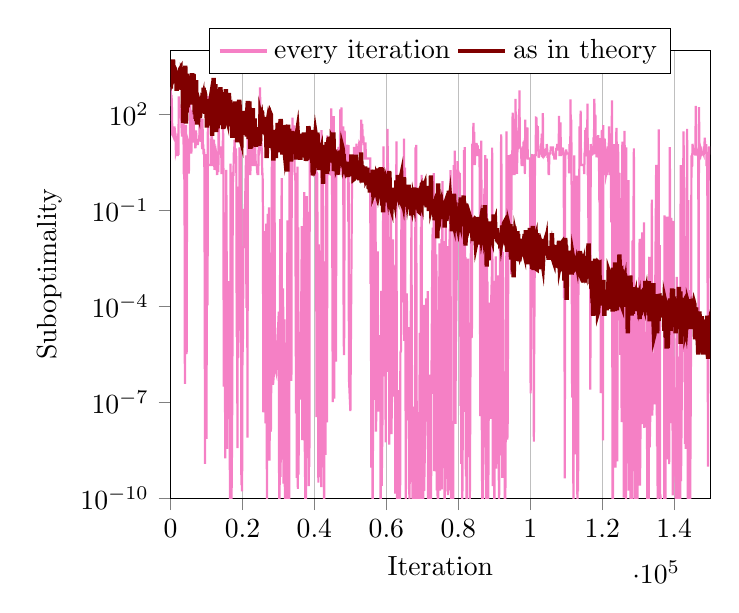
\begin{tikzpicture}

\begin{axis}[
legend cell align={left},
legend columns=2,
legend entries={{every iteration},{as in theory}},
legend style={at={(0.5,1.05)}, anchor=north},
tick align=outside,
tick pos=left,
xlabel={Iteration},
xmajorgrids,
xmin=0, xmax=150000,
ylabel={Suboptimality},
yminorgrids,
ymin=1e-10, ymax=10000,
ymode=log
]
\addlegendimage{no markers, very thick , magenta!50!white}
\addlegendimage{no markers, ultra thick, red!50!black}

\addplot [thick, magenta!50!white]
table [row sep=\\]{%
0	706.11181882878 \\
100	458.932919775816 \\
200	366.320293458517 \\
300	364.133825139994 \\
400	144.395995143052 \\
500	22.6398249134763 \\
600	21.7335473172061 \\
700	21.7764466837689 \\
800	19.8911266186878 \\
900	18.7006898150175 \\
1000	22.1843963351203 \\
1100	41.250606463389 \\
1200	32.0008860767739 \\
1300	25.9512779408942 \\
1400	17.782654723771 \\
1500	6.83467271422705 \\
1600	7.74595507644335 \\
1700	6.31161027625421 \\
1800	12.7172419809431 \\
1900	5.31709817124283 \\
2000	5.31785346208562 \\
2100	24.6167129785681 \\
2200	5.35760845886034 \\
2300	356.244410835228 \\
2400	118.26583917367 \\
2500	200.073538536912 \\
2600	95.7292470875618 \\
2700	98.6174143455464 \\
2800	93.7124140701999 \\
2900	82.6569999672574 \\
3000	71.3632151488055 \\
3100	33.6903477961896 \\
3200	19.7643668853379 \\
3300	684.145240489255 \\
3400	54.0433739742039 \\
3500	54.0430541971436 \\
3600	53.8834169295769 \\
3700	1.3949832604776 \\
3800	1.35209303559168 \\
3900	0.624650832382031 \\
4000	3.8096186472103e-07 \\
4100	1.44750525995551 \\
4200	0.00515501969493926 \\
4300	45.8003532324437 \\
4400	3.24793654726818e-06 \\
4500	3.88305852538906e-06 \\
4600	5.1901091253203 \\
4700	9.05332173064744 \\
4800	14.7765624689855 \\
4900	13.2870942707159 \\
5000	5.49158055403677 \\
5100	1.38164325680555 \\
5200	9.06469357638707 \\
5300	9.04063711161871 \\
5400	9.0406371072786 \\
5500	403.899456710271 \\
5600	9.84775182828889 \\
5700	6.3126120813904 \\
5800	6.31664838344295 \\
5900	17.1570650043759 \\
6000	81.0100036906515 \\
6100	80.9286338269303 \\
6200	130.714506854227 \\
6300	12.8305178067094 \\
6400	80.9284283863235 \\
6500	33.6754742543708 \\
6600	27.1149530399452 \\
6700	26.9907407859573 \\
6800	21.3659205554904 \\
6900	8.59229505819894 \\
7000	10.7281311626102 \\
7100	30.784785949756 \\
7200	15.2807721779427 \\
7300	14.0215376881242 \\
7400	13.9894719300137 \\
7500	11.6561163302613 \\
7600	11.6371774107356 \\
7700	15.5125133286492 \\
7800	15.5140927366701 \\
7900	15.5108051223433 \\
8000	15.510801808723 \\
8100	79.4935140879898 \\
8200	90.7883655884252 \\
8300	24.5084882459123 \\
8400	13.7528413169566 \\
8500	16.810564918811 \\
8600	23.4353772582544 \\
8700	21.7000751776686 \\
8800	8.09108234660016 \\
8900	72.0331285083776 \\
9000	7.9477496495565 \\
9100	11.2482378492459 \\
9200	5.52604633005103 \\
9300	7.99444693542682 \\
9400	5.52524974476546 \\
9500	0.000808694971055957 \\
9600	1.18961906991899e-09 \\
9700	5.20475250458185 \\
9800	5.18746947106774 \\
9900	0.00671890104058548 \\
10000	7.27595761418343e-09 \\
10100	0.000804481249360833 \\
10200	0.000238434473430971 \\
10300	0.000107054434920428 \\
10400	368.138078169261 \\
10500	2.78589195563109 \\
10600	2.57914148923373 \\
10700	2.57883931135802 \\
10800	2.57883931104152 \\
10900	2.57883931103788 \\
11000	2.57883931877586 \\
11100	2.57883931466858 \\
11200	2.57883939014573 \\
11300	2.57883931103424 \\
11400	74.2774196598402 \\
11500	22.1469549426001 \\
11600	2.57886365136801 \\
11700	16.3154416486177 \\
11800	5.7152181716192 \\
11900	2.57886011907613 \\
12000	2.57942999093939 \\
12100	15.919517973256 \\
12200	1.81300861609634 \\
12300	7.03033110281831 \\
12400	5.93368969191215 \\
12500	5.93337782299204 \\
12600	7.04381109424139 \\
12700	5.9333890418784 \\
12800	5.93337668547247 \\
12900	1.35207389274365 \\
13000	1.35697926734065 \\
13100	3.39877482865631 \\
13200	2.57886781985508 \\
13300	1.55744925530234 \\
13400	123.657661670182 \\
13500	5.9336908553596 \\
13600	5.93380836869255 \\
13700	5.93337731518477 \\
13800	9.83551774241641 \\
13900	5.93369056994197 \\
14000	8.07647181886568 \\
14100	8.16492060941164 \\
14200	1.35212555946418 \\
14300	5.08428000359709 \\
14400	3.44402219118274 \\
14500	2.57957197805081 \\
14600	73.0030892485083 \\
14700	2.57883980319093 \\
14800	3.10905306832865e-07 \\
14900	0.00506878650776343 \\
15000	0.0190726138462196 \\
15100	0.00539027158083627 \\
15200	1.78624759428203e-09 \\
15300	-3.63797880709171e-12 \\
15400	-3.63797880709171e-12 \\
15500	1.81885515122485 \\
15600	0.0104984676872846 \\
15700	3.54702933691442e-09 \\
15800	2.06091135623865e-06 \\
15900	3.23627282341477e-05 \\
16000	4.2211395339109e-06 \\
16100	0.000605309316597413 \\
16200	2.39790460909717e-06 \\
16300	0.000131169093947392 \\
16400	1.36038579512388e-07 \\
16500	-7.27595761418343e-12 \\
16600	3.63797880709171e-12 \\
16700	2.85960099315707 \\
16800	0.0636850832634082 \\
16900	1.09139364212751e-11 \\
17000	0 \\
17100	5.78074832446873e-09 \\
17200	1.87711702892557e-06 \\
17300	0.504788736790942 \\
17400	1.37112728069769 \\
17500	1.35207319103938 \\
17600	5.93834684234025 \\
17700	5.93382683410164 \\
17800	15.8971553375341 \\
17900	7.94734590741064 \\
18000	7.9473439902722 \\
18100	7.9473409473685 \\
18200	7.94734094735395 \\
18300	2.7003632875967 \\
18400	1.09110187622719e-05 \\
18500	0.542503181655775 \\
18600	3.69618646800518e-09 \\
18700	0.197064677464368 \\
18800	2.42378882830963e-06 \\
18900	0 \\
19000	0.00348405326440115 \\
19100	1.73901826201472e-05 \\
19200	9.21918824856039 \\
19300	5.93369017541409 \\
19400	5.93368973447286 \\
19500	5.93901292937517 \\
19600	0.000230197761993622 \\
19700	2.61934474110603e-10 \\
19800	0.000110576933366247 \\
19900	1.67347025126219e-10 \\
20000	9.65958679444157e-06 \\
20100	3.76256502931938e-06 \\
20200	0.000252126697887434 \\
20300	0.110168077222625 \\
20400	0.0208205640956294 \\
20500	0.00660961203175248 \\
20600	0 \\
20700	0 \\
20800	0 \\
20900	0 \\
21000	5.18746574042598 \\
21100	8.9415490947431e-05 \\
21200	0.00128859144024318 \\
21300	0.239601294855674 \\
21400	7.97808752395213e-09 \\
21500	20.7746001105479 \\
21600	10.8253011397974 \\
21700	2.5788731628345 \\
21800	2.57883967104499 \\
21900	8.62016245032646 \\
22000	1.35208917219643 \\
22100	1.35406772166607 \\
22200	1.35212768841302 \\
22300	41.3797144319215 \\
22400	7.94735641383159 \\
22500	7.94618312385865 \\
22600	17.5422870964721 \\
22700	9.83551717034425 \\
22800	2.80027105774207 \\
22900	2.57884010041016 \\
23000	2.57883931104152 \\
23100	2.57884069035572 \\
23200	2.5788398446748 \\
23300	2.57884112512693 \\
23400	29.6315062577924 \\
23500	48.2952694843771 \\
23600	5.18746428519808 \\
23700	2.77092770164745 \\
23800	2.57892133114728 \\
23900	2.57883936436338 \\
24000	2.57883931104516 \\
24100	1.55831174600098 \\
24200	1.35208644044542 \\
24300	1.35208458696798 \\
24400	1.35207442629689 \\
24500	9.38314906861342 \\
24600	5.76692697591352 \\
24700	6.41820881455715 \\
24800	193.472852049999 \\
24900	685.530697469974 \\
25000	9.83552329897066 \\
25100	9.8357318166527 \\
25200	17.3682388028901 \\
25300	10.1632626674873 \\
25400	6.80737265442804 \\
25500	1.35456190076729 \\
25600	1.35207318134053 \\
25700	0.077699850226054 \\
25800	4.91017999593168e-08 \\
25900	1.56105670612305e-07 \\
26000	0.00534263333247509 \\
26100	9.39799683692399e-05 \\
26200	0.000160533287271392 \\
26300	0.0220869861077517 \\
26400	2.21043592318892e-08 \\
26500	0 \\
26600	0.0381180773292726 \\
26700	8.79636500030756e-05 \\
26800	7.27595761418343e-11 \\
26900	-3.63797880709171e-12 \\
27000	0.0772607732687902 \\
27100	1.38869945658371e-05 \\
27200	2.63461843132973e-05 \\
27300	0.000478189129353268 \\
27400	0.122065377952822 \\
27500	1.51339918375015e-09 \\
27600	-3.63797880709171e-12 \\
27700	2.29334546020254e-07 \\
27800	0 \\
27900	1.20890035759658e-08 \\
28000	5.13791746925563e-07 \\
28100	-7.27595761418343e-12 \\
28200	25.902530968815 \\
28300	0.0151031112764031 \\
28400	0.000196416411199607 \\
28500	3.54557414539158e-07 \\
28600	0 \\
28700	0 \\
28800	9.65646904660389e-07 \\
28900	18.6299063920014 \\
29000	4.07499028369784e-05 \\
29100	1.15431612357497e-06 \\
29200	0 \\
29300	0 \\
29400	8.34548700368032e-07 \\
29500	0 \\
29600	-3.63797880709171e-12 \\
29700	0 \\
29800	0 \\
29900	0 \\
30000	0 \\
30100	6.84153492329642e-05 \\
30200	1.20053300634027e-10 \\
30300	3.63797880709171e-12 \\
30400	0 \\
30500	0.0527262009491096 \\
30600	4.69299266114831e-10 \\
30700	-3.63797880709171e-12 \\
30800	-3.63797880709171e-12 \\
30900	0.999172102201555 \\
31000	1.63709046319127e-09 \\
31100	-3.63797880709171e-12 \\
31200	1.5919613360893e-06 \\
31300	0.000364204272045754 \\
31400	2.91038304567337e-10 \\
31500	7.71753548178822e-07 \\
31600	0 \\
31700	3.90897475881502e-05 \\
31800	3.27418092638254e-11 \\
31900	7.2717375587672e-06 \\
32000	7.27595761418343e-12 \\
32100	7.13193003321066e-07 \\
32200	-3.63797880709171e-12 \\
32300	3.63797880709171e-12 \\
32400	2.67784344032407e-07 \\
32500	0.0480681582157558 \\
32600	5.61569322599098e-07 \\
32700	0.00322525984302047 \\
32800	1.2105010682717e-07 \\
32900	0 \\
33000	3.63797880709171e-12 \\
33100	6.3409066736931 \\
33200	6.28102431057778 \\
33300	5.93368980384912 \\
33400	7.72508393636599 \\
33500	2.57883938489249 \\
33600	4.71165549242869e-07 \\
33700	5.25480021346448 \\
33800	6.3904081496803 \\
33900	78.248059460846 \\
34000	4.33417665561865 \\
34100	7.17287332627166 \\
34200	9.83552107374999 \\
34300	4.39353869194383 \\
34400	44.8306644679287 \\
34500	1.35244708311802 \\
34600	1.35207318098401 \\
34700	1.35207318065659 \\
34800	6.46167136437725e-05 \\
34900	4.54783730674535e-08 \\
35000	0.000538212614628719 \\
35100	4.40195435658097e-10 \\
35200	1.51946733240038e-06 \\
35300	2.30545584656647 \\
35400	2.00088834390044e-10 \\
35500	0.0290886601796956 \\
35600	5.5297277867794e-10 \\
35700	1.28984538605437e-06 \\
35800	0 \\
35900	0 \\
36000	1.21683115139604e-07 \\
36100	-7.27595761418343e-12 \\
36200	-3.63797880709171e-12 \\
36300	0 \\
36400	0.000516508502187207 \\
36500	0.0318168063895428 \\
36600	6.55927578918636e-09 \\
36700	0 \\
36800	-7.27595761418343e-12 \\
36900	0 \\
37000	0.00143875402864069 \\
37100	0.0200666419696063 \\
37200	0.365842599290772 \\
37300	9.46965883485973e-09 \\
37400	-3.63797880709171e-12 \\
37500	0 \\
37600	3.63797880709171e-12 \\
37700	0 \\
37800	6.66448358970229e-05 \\
37900	0.274572404927312 \\
38000	7.87622411735356e-09 \\
38100	5.96222525928169e-06 \\
38200	0 \\
38300	0.00278996945780818 \\
38400	2.40106601268053e-10 \\
38500	0.0894023516520974 \\
38600	9.64064383879304e-10 \\
38700	5.18980549719345 \\
38800	1.3521132897622 \\
38900	2.57889370343764 \\
39000	2.57883931107062 \\
39100	2.57883931104152 \\
39200	2.57884820483741 \\
39300	5.83461238876043 \\
39400	1.45132417971399 \\
39500	1.40484852671216 \\
39600	1.35207728042951 \\
39700	2.58508809202613 \\
39800	1.35209297386609 \\
39900	1.35339299704719 \\
40000	1.3525377744154 \\
40100	1.3779895963271 \\
40200	2.7611810119779 \\
40300	2.57883952738121 \\
40400	2.57945799715162 \\
40500	0.015815689410374 \\
40600	3.48118192050606e-08 \\
40700	1.44062749447039 \\
40800	1.35207320897825 \\
40900	0.000138132862048224 \\
41000	0.00207236503774766 \\
41100	3.09228198602796e-10 \\
41200	0.00849037010993925 \\
41300	0.0033488307526568 \\
41400	2.11366568692029e-09 \\
41500	0 \\
41600	0.000442360393208219 \\
41700	4.62023308500648e-10 \\
41800	0.000196146178495837 \\
41900	2.25554686039686e-10 \\
42000	31.7938721368082 \\
42100	3.69938788935542e-07 \\
42200	0.0489560210262425 \\
42300	10.1298969096824 \\
42400	0.00651900492448476 \\
42500	1.46888523886446e-05 \\
42600	6.83940015733242e-09 \\
42700	3.63797880709171e-12 \\
42800	3.27454472426325e-08 \\
42900	9.18000296223909e-07 \\
43000	0.00252767673373455 \\
43100	2.30284058488905e-09 \\
43200	0.0388976370522869 \\
43300	9.23523756153008 \\
43400	3.67236365129429 \\
43500	2.3523170966655e-08 \\
43600	21.7681133584556 \\
43700	1.35383489870947 \\
43800	1.35207318577886 \\
43900	1.35207318065659 \\
44000	1.35207318065659 \\
44100	1.35207318065295 \\
44200	1.35207318065295 \\
44300	1.35207332576101 \\
44400	1.35207318066023 \\
44500	1.42298817265691 \\
44600	1.35330976735713 \\
44700	152.599603344584 \\
44800	2.57884154567 \\
44900	1.35208430794228 \\
45000	0.000686096915160306 \\
45100	1.02547346614301e-07 \\
45200	-3.63797880709171e-12 \\
45300	8.58301063999534e-06 \\
45400	86.7548017446061 \\
45500	1.31360138766468e-07 \\
45600	0.00426498168963008 \\
45700	0.0537874853798712 \\
45800	1.36068684138081 \\
45900	1.35207318501853 \\
46000	1.87805198947899e-06 \\
46100	5.33315614948151 \\
46200	7.86112523066186 \\
46300	3.60579681214585 \\
46400	1.35207686512877 \\
46500	1.35210827435731 \\
46600	1.35207318070752 \\
46700	9.50193826329269 \\
46800	1.35434486155646 \\
46900	1.35207318155153 \\
47000	1.35207371923025 \\
47100	5.93435742993461 \\
47200	141.485603234076 \\
47300	7.94736782298423 \\
47400	7.95541294810755 \\
47500	163.974683695091 \\
47600	2.57884122110772 \\
47700	2.57883931103788 \\
47800	1.35241111718642 \\
47900	1.35611043620884 \\
48000	41.5203664058899 \\
48100	0.000227912394620944 \\
48200	2.99303792417049e-06 \\
48300	1.94813073903788e-05 \\
48400	30.6078390144539 \\
48500	6.29492712243155 \\
48600	5.93368980976084 \\
48700	3.16547227395858 \\
48800	2.57883991167182 \\
48900	2.57883931104152 \\
49000	2.57883931104516 \\
49100	11.2475772537437 \\
49200	1.35207405544861 \\
49300	4.55602353380164 \\
49400	0.0442882784336689 \\
49500	10.7624414642123 \\
49600	5.64526999369264e-07 \\
49700	-3.63797880709171e-12 \\
49800	-3.63797880709171e-12 \\
49900	0 \\
50000	5.37329469807446e-08 \\
50100	-7.27595761418343e-12 \\
50200	0 \\
50300	0 \\
50400	0 \\
50500	4.37057953511248 \\
50600	1.35394365859611 \\
50700	1.35239627027477 \\
50800	1.3520731807148 \\
50900	1.35207318065659 \\
51000	9.52740778697989 \\
51100	2.57903387927945 \\
51200	2.5788393113944 \\
51300	2.57884778513471 \\
51400	6.35490475143888 \\
51500	2.57920618591015 \\
51600	2.57883931108881 \\
51700	12.0805076164652 \\
51800	5.19407325272186 \\
51900	9.04064467448916 \\
52000	9.04063710728951 \\
52100	9.04063710728587 \\
52200	9.04063710728951 \\
52300	5.99189238354302 \\
52400	9.06094964801741 \\
52500	7.94617149263286 \\
52600	14.8320177963869 \\
52700	1.35282402495795 \\
52800	1.35207318195171 \\
52900	1.35208367768064 \\
53000	66.8840265793951 \\
53100	23.676470002014 \\
53200	22.8918563666593 \\
53300	49.3104335766729 \\
53400	18.0075419961904 \\
53500	12.4510907325821 \\
53600	20.6908488331392 \\
53700	11.6362844095929 \\
53800	11.6359671240425 \\
53900	11.6372025600322 \\
54000	4.14046687406881 \\
54100	4.14005519054263 \\
54200	13.0767269230455 \\
54300	4.14172378341755 \\
54400	4.14000251542166 \\
54500	4.14071966734264 \\
54600	4.14000251449397 \\
54700	4.14000251326433 \\
54800	4.13768416839594 \\
54900	4.13766740024585 \\
55000	4.13772298413824 \\
55100	4.13766740035499 \\
55200	4.1376674002131 \\
55300	4.13766740021674 \\
55400	4.1376686007352 \\
55500	4.13766740020947 \\
55600	0.000499020839924924 \\
55700	0.193372908983292 \\
55800	9.24046617001295e-10 \\
55900	9.87056409940124e-08 \\
56000	-3.63797880709171e-12 \\
56100	1.14852446131408e-06 \\
56200	3.63797880709171e-12 \\
56300	-3.63797880709171e-12 \\
56400	0.0811524621713033 \\
56500	0.192600539045088 \\
56600	4.93945117341354e-06 \\
56700	0.000337474539264804 \\
56800	1.2013697414659e-07 \\
56900	0.0201716810843209 \\
57000	0.378698390326463 \\
57100	1.21435732580721e-08 \\
57200	0 \\
57300	0 \\
57400	-7.27595761418343e-12 \\
57500	1.62922879098915e-06 \\
57600	0.00516889896971406 \\
57700	2.6544148568064e-07 \\
57800	-3.63797880709171e-12 \\
57900	5.16556610818952e-08 \\
58000	0 \\
58100	0 \\
58200	-3.63797880709171e-12 \\
58300	1.25257538456935e-05 \\
58400	7.27595761418343e-12 \\
58500	0 \\
58600	0.000302871932944981 \\
58700	2.47382558882236e-10 \\
58800	-3.63797880709171e-12 \\
58900	2.05982360057533e-08 \\
59000	2.09073732548859e-05 \\
59100	0.0681638785172254 \\
59200	9.78041434730039 \\
59300	6.44380634184927e-07 \\
59400	0.011130244951346 \\
59500	1.73704902408645e-05 \\
59600	0 \\
59700	0.164421783632861 \\
59800	5.63886715099216e-09 \\
59900	-3.63797880709171e-12 \\
60000	1.20313252722917 \\
60100	8.93938704393804e-07 \\
60200	-3.63797880709171e-12 \\
60300	34.5485131659043 \\
60400	3.88820735525223 \\
60500	1.35261121403892 \\
60600	0.00126290717162192 \\
60700	0.00149727899770369 \\
60800	4.82395989820361e-09 \\
60900	0.00212471085978905 \\
61000	2.34216349781491e-06 \\
61100	0.00123815871120314 \\
61200	1.80996357812546e-06 \\
61300	0.131637408299866 \\
61400	1.01099431049079e-08 \\
61500	0 \\
61600	-3.63797880709171e-12 \\
61700	1.49713378050365e-06 \\
61800	0.0122573593871493 \\
61900	1.49844709085301e-07 \\
62000	5.82398206461221e-06 \\
62100	-3.63797880709171e-12 \\
62200	-7.27595761418343e-12 \\
62300	0.00188199988406268 \\
62400	9.68489148363005e-05 \\
62500	1.41881173476577e-10 \\
62600	2.50526500167325e-06 \\
62700	0 \\
62800	14.1927896991801 \\
62900	1.26514350995421e-07 \\
63000	3.63797880709171e-12 \\
63100	-7.27595761418343e-12 \\
63200	0 \\
63300	0 \\
63400	2.71029421128333e-09 \\
63500	2.40412191487849e-07 \\
63600	0 \\
63700	-3.63797880709171e-12 \\
63800	3.63797880709171e-12 \\
63900	3.56993405148387e-06 \\
64000	-3.63797880709171e-12 \\
64100	4.22844823333435e-06 \\
64200	1.35955470826593 \\
64300	1.43839027509603 \\
64400	1.35207318066023 \\
64500	1.7278103352146 \\
64600	1.35207318382891 \\
64700	0.000133387376990868 \\
64800	0.000295895144517999 \\
64900	17.1660912940715 \\
65000	8.29670170787722e-06 \\
65100	0 \\
65200	2.12141502909071 \\
65300	6.09415583312511e-05 \\
65400	4.36557456851006e-11 \\
65500	-3.63797880709171e-12 \\
65600	0 \\
65700	0.000251691941230092 \\
65800	1.43132638186216e-07 \\
65900	1.81826180778444e-06 \\
66000	-3.63797880709171e-12 \\
66100	2.7292117010802e-08 \\
66200	0 \\
66300	2.2510841517942e-05 \\
66400	4.72937244921923e-11 \\
66500	5.78438630327582e-10 \\
66600	-3.63797880709171e-12 \\
66700	-7.27595761418343e-12 \\
66800	-3.63797880709171e-12 \\
66900	0 \\
67000	0.100580286169134 \\
67100	3.20142135024071e-10 \\
67200	1.09139364212751e-09 \\
67300	0 \\
67400	3.63797880709171e-12 \\
67500	0 \\
67600	7.35235516913235e-08 \\
67700	3.63797880709171e-12 \\
67800	0 \\
67900	3.63797880709171e-12 \\
68000	0 \\
68100	9.24614994881267 \\
68200	1.90307000593748e-05 \\
68300	10.9035907495527 \\
68400	2.0818697521463e-07 \\
68500	0 \\
68600	0 \\
68700	3.63797880709171e-12 \\
68800	0 \\
68900	0 \\
69000	0 \\
69100	0 \\
69200	8.68494680617005e-08 \\
69300	1.48254766827449e-05 \\
69400	3.63797880709171e-12 \\
69500	-3.63797880709171e-12 \\
69600	0.0303877778860624 \\
69700	1.96450855582952e-10 \\
69800	1.26234853784626 \\
69900	7.41783878766e-09 \\
70000	0 \\
70100	-3.63797880709171e-12 \\
70200	3.63797880709171e-12 \\
70300	-3.63797880709171e-12 \\
70400	0.000110974247945705 \\
70500	1.70985003933311e-10 \\
70600	0 \\
70700	0 \\
70800	0 \\
70900	0 \\
71000	2.12206941796467e-07 \\
71100	0.000177265741513111 \\
71200	6.20872742729262e-06 \\
71300	9.79892865871079e-06 \\
71400	-3.63797880709171e-12 \\
71500	0.000297501759632723 \\
71600	4.00177668780088e-11 \\
71700	-3.63797880709171e-12 \\
71800	0 \\
71900	0 \\
72000	7.27613951312378e-07 \\
72100	0 \\
72200	0 \\
72300	-3.63797880709171e-12 \\
72400	3.63797880709171e-12 \\
72500	1.10801920527592e-07 \\
72600	-3.63797880709171e-12 \\
72700	0 \\
72800	0.0098154258885188 \\
72900	0.0285091683326755 \\
73000	1.82742951437831e-07 \\
73100	0.000191662031284068 \\
73200	1.43118579937436 \\
73300	7.05767888575792e-10 \\
73400	1.90579157788306e-07 \\
73500	1.47752398333978e-05 \\
73600	0.103461149312352 \\
73700	3.15776560455561e-09 \\
73800	0 \\
73900	0.00420300224504899 \\
74000	1.78260961547494e-10 \\
74100	1.84668388101272e-05 \\
74200	3.27418092638254e-10 \\
74300	0 \\
74400	3.63797880709171e-12 \\
74500	2.96724465442821e-07 \\
74600	0 \\
74700	-3.63797880709171e-12 \\
74800	0.00918678185189492 \\
74900	1.74622982740402e-10 \\
75000	-3.63797880709171e-12 \\
75100	-3.63797880709171e-12 \\
75200	0 \\
75300	0.012409110498993 \\
75400	1.92812876775861e-10 \\
75500	0.00103959027546807 \\
75600	0.812640406118589 \\
75700	5.94445737078786e-09 \\
75800	0 \\
75900	0 \\
76000	0.0108636142213072 \\
76100	3.68163455277681e-09 \\
76200	3.63797880709171e-12 \\
76300	0.000151426018419443 \\
76400	1.67347025126219e-10 \\
76500	0.1380517570542 \\
76600	1.58433977048844e-08 \\
76700	8.23307345854118e-07 \\
76800	-3.63797880709171e-12 \\
76900	-3.63797880709171e-12 \\
77000	0.00753105252806563 \\
77100	1.2732925824821e-10 \\
77200	0 \\
77300	0 \\
77400	0 \\
77500	-3.63797880709171e-12 \\
77600	0.0263656915703905 \\
77700	1.78260961547494e-10 \\
77800	1.78698841710866 \\
77900	2.79501546174288e-06 \\
78000	1.09139364212751e-11 \\
78100	-7.27595761418343e-12 \\
78200	0 \\
78300	-3.63797880709171e-12 \\
78400	0 \\
78500	-3.63797880709171e-12 \\
78600	3.63797880709171e-12 \\
78700	2.55320566877344 \\
78800	8.14349223219324e-05 \\
78900	1.12501584226266e-06 \\
79000	7.24059520060109 \\
79100	0.0198331461906491 \\
79200	2.11875885725021e-08 \\
79300	4.44731995230541e-06 \\
79400	0 \\
79500	-7.27595761418343e-12 \\
79600	0.00257589683315018 \\
79700	1.35207501998229 \\
79800	3.418333310874 \\
79900	1.35296874352571 \\
80000	1.35207318091125 \\
80100	1.48000787504134 \\
80200	1.3520731808494 \\
80300	1.35207318542962 \\
80400	1.35207318065659 \\
80500	0.452018973966915 \\
80600	7.70851329434663e-08 \\
80700	0.0035514731935109 \\
80800	1.19325704872608e-09 \\
80900	0.0517407752340659 \\
81000	0.000290922820568085 \\
81100	4.00177668780088e-11 \\
81200	0 \\
81300	0 \\
81400	1.36120324896183e-05 \\
81500	4.13820816902444e-06 \\
81600	7.50945024149769 \\
81700	5.00913301948458e-08 \\
81800	9.3950291632791 \\
81900	6.99474185239524e-08 \\
82000	0.00341782635223353 \\
82100	4.8748916015029e-10 \\
82200	6.01254214416258e-06 \\
82300	3.63797880709171e-12 \\
82400	4.90399543195963e-08 \\
82500	-3.63797880709171e-12 \\
82600	0 \\
82700	0.00310216057550861 \\
82800	1.96087057702243e-09 \\
82900	-3.63797880709171e-12 \\
83000	2.28519638767466e-07 \\
83100	3.10496761812828e-05 \\
83200	5.45696821063757e-11 \\
83300	-3.63797880709171e-12 \\
83400	7.46976002119482e-06 \\
83500	0.0119498423191544 \\
83600	0.000364482762961416 \\
83700	1.01945988717489e-05 \\
83800	2.52830504905432e-05 \\
83900	11.2674876521523 \\
84000	11.6304766397407 \\
84100	11.6417330527111 \\
84200	53.6907603446234 \\
84300	11.2336930398887 \\
84400	27.8865780786837 \\
84500	5.1884097887596 \\
84600	2.57917057284067 \\
84700	10.1519829282151 \\
84800	4.90122465883178 \\
84900	9.88336346992946 \\
85000	11.6268528166038 \\
85100	11.6259332029367 \\
85200	10.1845488483305 \\
85300	9.83551731676562 \\
85400	9.8355167849877 \\
85500	4.87569152820652 \\
85600	5.93917266984499 \\
85700	8.16838231289876 \\
85800	6.03654588595236 \\
85900	5.55969104574615 \\
86000	0.041540426274878 \\
86100	3.7245627027005e-08 \\
86200	0 \\
86300	0.000722812965250341 \\
86400	14.8189374063804 \\
86500	1.40578777063638e-07 \\
86600	0 \\
86700	3.63797880709171e-12 \\
86800	0 \\
86900	0 \\
87000	1.41179043566808e-07 \\
87100	6.51934678899124e-05 \\
87200	0.242611275545642 \\
87300	0.478429932321887 \\
87400	3.92174115404487e-09 \\
87500	5.2471101971787 \\
87600	1.77563561010174e-06 \\
87700	3.63797880709171e-12 \\
87800	-3.63797880709171e-12 \\
87900	4.05400718040619 \\
88000	1.21633602248039e-05 \\
88100	0.000584743000217713 \\
88200	2.29007127927616e-07 \\
88300	3.63797880709171e-12 \\
88400	1.32677087094635e-08 \\
88500	0 \\
88600	-7.27595761418343e-12 \\
88700	-3.63797880709171e-12 \\
88800	0.000130483360408107 \\
88900	4.42094096797518e-06 \\
89000	3.05917637888342e-08 \\
89100	0 \\
89200	0.00046792399007245 \\
89300	4.68482794531155e-05 \\
89400	8.96514873993146 \\
89500	0.000151713462400949 \\
89600	2.43744580075145e-10 \\
89700	0 \\
89800	-3.63797880709171e-12 \\
89900	5.62846980756149e-06 \\
90000	3.63797880709171e-12 \\
90100	-7.27595761418343e-12 \\
90200	0.000623625575826736 \\
90300	3.78469849238172e-07 \\
90400	0.00362342449807329 \\
90500	8.47649062052369e-10 \\
90600	-7.27595761418343e-12 \\
90700	-3.63797880709171e-12 \\
90800	6.14807504462078e-07 \\
90900	0.000918223115149885 \\
91000	1.24418875202537e-09 \\
91100	8.1799371400848e-06 \\
91200	1.3591652532341e-05 \\
91300	3.63797880709171e-12 \\
91400	0 \\
91500	-7.27595761418343e-12 \\
91600	0.0101873717976559 \\
91700	2.20825313590467e-09 \\
91800	0.000651172158541158 \\
91900	23.3931416151754 \\
92000	1.3629157915675 \\
92100	0.000349021109286696 \\
92200	4.40195435658097e-10 \\
92300	2.16823536902666e-09 \\
92400	0.00496757094879285 \\
92500	0.000249959011853207 \\
92600	5.299189069774e-07 \\
92700	5.73654688196257e-07 \\
92800	1.00844772532582e-08 \\
92900	0 \\
93000	3.63797880709171e-12 \\
93100	0 \\
93200	4.6369677875191e-08 \\
93300	9.45219653658569e-08 \\
93400	28.90079599413 \\
93500	0.024071100702713 \\
93600	6.90488377586007e-09 \\
93700	9.66247171163559e-09 \\
93800	0 \\
93900	0.00667086932662642 \\
94000	5.2022231148876 \\
94100	1.35270063496137 \\
94200	1.35207318231551 \\
94300	1.35207322315182 \\
94400	1.590008119907 \\
94500	5.4745997928112 \\
94600	1.35207318903122 \\
94700	0.000993517343886197 \\
94800	5.18756355351434 \\
94900	5.18746286416354 \\
95000	3.4049213679973 \\
95100	111.824691416434 \\
95200	2.58803960612204 \\
95300	1.35400264117561 \\
95400	1.35207318206085 \\
95500	1.35207318093308 \\
95600	1.35207323279974 \\
95700	10.5582521624929 \\
95800	11.6261289393697 \\
95900	298.986213783141 \\
96000	22.1344939664268 \\
96100	10.9389470518945 \\
96200	2.60385977014084 \\
96300	1.35481852514931 \\
96400	6.17121635413787 \\
96500	8.09951534829452 \\
96600	30.3697066159839 \\
96700	9.83552271778899 \\
96800	96.7702918489558 \\
96900	9.14258000431073 \\
97000	548.305798855301 \\
97100	9.04064758533787 \\
97200	9.04063710729315 \\
97300	9.04063710728587 \\
97400	7.90884723260388 \\
97500	4.67048478403012 \\
97600	2.58287383406787 \\
97700	2.57883931581091 \\
97800	2.5788394817173 \\
97900	2.5788457435483 \\
98000	2.5788395270356 \\
98100	13.9254514621425 \\
98200	2.57884094742622 \\
98300	2.58228112695724 \\
98400	15.2515307076501 \\
98500	1.35209606746139 \\
98600	66.9134894894923 \\
98700	6.09348177071297 \\
98800	7.1558786997557 \\
98900	5.52604808340766 \\
99000	4.14033059307621 \\
99100	20.9469158527863 \\
99200	38.4656420335887 \\
99300	4.14008457347154 \\
99400	4.14000251335528 \\
99500	4.14000251326433 \\
99600	4.14000251326797 \\
99700	4.1400025132607 \\
99800	4.15245913503895 \\
99900	4.14000255702194 \\
100000	0.370907321568666 \\
100100	1.91757862921804e-07 \\
100200	0 \\
100300	0 \\
100400	-3.63797880709171e-12 \\
100500	5.21206351866567 \\
100600	5.18746288508555 \\
100700	2.58301561685948 \\
100800	1.35364859185574 \\
100900	1.68543874390161 \\
101000	5.93718141317368e-09 \\
101100	1.94141975953244e-05 \\
101200	0.000131385058921296 \\
101300	5.20308843108432 \\
101400	5.18746290102354 \\
101500	5.21768172127486 \\
101600	77.2824258201326 \\
101700	76.6213094290724 \\
101800	37.3845620151587 \\
101900	23.19940674385 \\
102000	7.34259438084337 \\
102100	41.870842836739 \\
102200	9.84140888051115 \\
102300	4.70265677494535 \\
102400	4.66656433080061 \\
102500	4.90042794431065 \\
102600	5.93338613318338 \\
102700	7.95187555302982 \\
102800	5.93369010987954 \\
102900	5.9336955224062 \\
103000	9.84041239653743 \\
103100	12.6949441053366 \\
103200	24.419838767888 \\
103300	4.92927347264049 \\
103400	4.78356157804956 \\
103500	106.952659258081 \\
103600	4.77246839219879 \\
103700	4.77183444536786 \\
103800	4.77061021500413 \\
103900	8.0051122228615 \\
104000	4.90872939451583 \\
104100	7.31688820722047 \\
104200	7.56292367975402 \\
104300	7.30013560433508 \\
104400	7.29791295508039 \\
104500	5.26121803526985 \\
104600	11.6325816714743 \\
104700	8.15981308560004 \\
104800	4.66781892839936 \\
104900	4.66781891834398 \\
105000	4.66781891834034 \\
105100	1.3521541279988 \\
105200	1.35300758069934 \\
105300	5.93378047772057 \\
105400	5.93368965824629 \\
105500	5.9336896580935 \\
105600	5.9383209737498 \\
105700	9.04169999890655 \\
105800	9.04063710848277 \\
105900	9.04063710728951 \\
106000	9.04031383125766 \\
106100	9.05334559342737 \\
106200	9.04031368135838 \\
106300	9.04031367404241 \\
106400	5.5261373999856 \\
106500	5.52524956563866 \\
106600	5.52524956460184 \\
106700	4.13793747768068 \\
106800	4.15953747195454 \\
106900	4.13766741858126 \\
107000	4.1376674002131 \\
107100	4.13766740021674 \\
107200	7.97163205021934 \\
107300	7.90827749474192 \\
107400	7.90698900340067 \\
107500	11.6259653045199 \\
107600	7.99415941641928 \\
107700	7.96969091782012 \\
107800	7.96963221973783 \\
107900	7.9696352855899 \\
108000	88.3859256532342 \\
108100	4.90113114045016 \\
108200	36.665675330587 \\
108300	4.90113661597206 \\
108400	54.8631635105194 \\
108500	4.90112945507644 \\
108600	6.86631748764557 \\
108700	5.93337718105249 \\
108800	5.93491112904303 \\
108900	5.93368965871196 \\
109000	5.94017811052618 \\
109100	9.04239260929899 \\
109200	5.58298638732595 \\
109300	5.5260462492879 \\
109400	0.000180273069418035 \\
109500	0.000535213392140577 \\
109600	4.2564352042973e-10 \\
109700	3.82066532639146 \\
109800	5.9394860919856 \\
109900	5.93368966389608 \\
110000	7.90908562649565 \\
110100	5.93400451185516 \\
110200	5.93368965835907 \\
110300	5.93368965809714 \\
110400	5.93491457635173 \\
110500	5.93337678843454 \\
110600	5.93337668545428 \\
110700	5.93337668545428 \\
110800	1.42113438485831 \\
110900	11.6592092736646 \\
111000	2.57884497050691 \\
111100	2.57883931247852 \\
111200	290.097728930294 \\
111300	2.57884365280188 \\
111400	66.8689673125846 \\
111500	0.402622022855212 \\
111600	5.86318492423743e-07 \\
111700	1.41830241773278e-07 \\
111800	-3.63797880709171e-12 \\
111900	1.02350531960838e-05 \\
112000	1.45519152283669e-11 \\
112100	-3.63797880709171e-12 \\
112200	5.15271681663216 \\
112300	5.3399708122015e-07 \\
112400	-3.63797880709171e-12 \\
112500	1.8021855794359e-06 \\
112600	0.00618084958477993 \\
112700	2.39015207625926e-09 \\
112800	0 \\
112900	1.20970841606322 \\
113000	5.45511793461628e-05 \\
113100	2.91038304567337e-11 \\
113200	0.000119034488307079 \\
113300	1.67347025126219e-10 \\
113400	0.0140663986931031 \\
113500	0.00296232653272455 \\
113600	0.157598692887404 \\
113700	41.2081457876411 \\
113800	5.1875566786548 \\
113900	5.18746436667425 \\
114000	128.569136225244 \\
114100	2.99378235166296 \\
114200	2.57884043792365 \\
114300	2.57884261723302 \\
114400	2.57883931104152 \\
114500	2.57913536138949 \\
114600	2.57883983141801 \\
114700	2.57894651556126 \\
114800	2.57883931105607 \\
114900	2.57982181377156 \\
115000	1.35234792160554 \\
115100	5.9392107548083 \\
115200	7.05215812640381 \\
115300	31.7495065826588 \\
115400	9.62967683115858 \\
115500	37.8121641352009 \\
115600	5.19592158947853 \\
115700	5.18746427264341 \\
115800	5.18766286658138 \\
115900	211.153345583283 \\
116000	1.35218034199715 \\
116100	1.35869875144272 \\
116200	0.00162299919611542 \\
116300	7.36734165582675 \\
116400	5.19207307697798 \\
116500	0.000775488537328783 \\
116600	1.15466784242744 \\
116700	2.50722223427147e-07 \\
116800	11.6295130894432 \\
116900	9.0406375277671 \\
117000	9.04248152678701 \\
117100	5.5275342719724 \\
117200	5.52525134844473 \\
117300	9.0406425411602 \\
117400	5.93430653493488 \\
117500	5.9336896593959 \\
117600	18.6798898304332 \\
117700	5.65606528744684 \\
117800	302.017607327249 \\
117900	76.6213841626777 \\
118000	76.6611544114276 \\
118100	95.5494388487714 \\
118200	11.7466607409588 \\
118300	10.0725681238218 \\
118400	4.8468851481739 \\
118500	4.84856776645393 \\
118600	4.85195441285396 \\
118700	4.84858963350416 \\
118800	4.849299920872 \\
118900	22.0872285977712 \\
119000	4.85036359327933 \\
119100	4.9053544800372 \\
119200	0.207952086628211 \\
119300	0.167247577828675 \\
119400	5.64805450267158e-05 \\
119500	17.7343781328564 \\
119600	1.94657332031056e-07 \\
119700	1.6228252206929e-05 \\
119800	0.000282709363091271 \\
119900	32.3659985247759 \\
120000	0.0827472411401686 \\
120100	0.0204241206265579 \\
120200	6.51562004350126e-09 \\
120300	45.6699001036686 \\
120400	1.3520736991195 \\
120500	1.35207318065659 \\
120600	1.3528755371517 \\
120700	16.9982247217667 \\
120800	9.83551685947532 \\
120900	8.02415399872552 \\
121000	5.93368968039795 \\
121100	1.35207345043091 \\
121200	1.55393927324621 \\
121300	1.35207318198081 \\
121400	1.35207318065659 \\
121500	1.35207318065659 \\
121600	9.83571497195953 \\
121700	4.66781913902378 \\
121800	4.66781891834398 \\
121900	41.8060754234975 \\
122000	5.18837765148783 \\
122100	6.88416470959055 \\
122200	1.35208459400019 \\
122300	1.35207318068933 \\
122400	1.35207318065659 \\
122500	0.0419937768820091 \\
122600	1.36377692724636 \\
122700	266.628656089244 \\
122800	1.59818919200916e-05 \\
122900	1.09139364212751e-11 \\
123000	3.63797880709171e-12 \\
123100	0.0325350870480179 \\
123200	6.42790837446228e-07 \\
123300	0 \\
123400	11.4963549287895 \\
123500	8.89122020453215e-08 \\
123600	0.00396631711919326 \\
123700	9.20408638194203e-10 \\
123800	0 \\
123900	24.9299835791462 \\
124000	37.2074615017336 \\
124100	0.000945016996411141 \\
124200	1.44063960760832e-09 \\
124300	1.35207394847384 \\
124400	11.5898700949692 \\
124500	1.35935982729279 \\
124600	1.35207319789333 \\
124700	1.35601766078253 \\
124800	1.35207318236644 \\
124900	0.0243311412123148 \\
125000	3.01465843222104e-06 \\
125100	0 \\
125200	2.89867384708486e-05 \\
125300	0.000324747557897354 \\
125400	2.41343514062464e-08 \\
125500	-3.63797880709171e-12 \\
125600	13.8381343182991 \\
125700	3.47042077919468e-06 \\
125800	4.25126199843362e-06 \\
125900	0.000298040213237982 \\
126000	1.0550138540566e-10 \\
126100	2.5465851649642e-09 \\
126200	29.7845100121413 \\
126300	1.35208409866027 \\
126400	0.758926349673857 \\
126500	4.9311674956698e-05 \\
126600	2.91038304567337e-11 \\
126700	9.11200130087309 \\
126800	8.53106030263007e-09 \\
126900	0.00233265334099997 \\
127000	1.25146470963955e-09 \\
127100	-7.27595761418343e-12 \\
127200	-3.63797880709171e-12 \\
127300	0.8730536611547 \\
127400	1.74622982740402e-10 \\
127500	-7.27595761418343e-12 \\
127600	-3.63797880709171e-12 \\
127700	0 \\
127800	7.29812491044868e-05 \\
127900	1.09139364212751e-11 \\
128000	8.80572770256549e-08 \\
128100	6.98942458257079e-05 \\
128200	3.63797880709171e-12 \\
128300	-7.27595761418343e-12 \\
128400	0.0111377503926633 \\
128500	9.77879244601354e-06 \\
128600	0 \\
128700	-3.63797880709171e-12 \\
128800	8.45885267100675 \\
128900	6.29150599706918e-06 \\
129000	7.27595761418343e-12 \\
129100	0 \\
129200	-3.63797880709171e-12 \\
129300	3.63797880709171e-12 \\
129400	8.79663275554776e-09 \\
129500	-7.27595761418343e-12 \\
129600	8.02298454800621e-05 \\
129700	3.63797880709171e-12 \\
129800	-7.27595761418343e-12 \\
129900	0 \\
130000	0 \\
130100	0 \\
130200	0 \\
130300	0.000348625268088654 \\
130400	0.0127443311866955 \\
130500	2.51020537689328e-10 \\
130600	0 \\
130700	0 \\
130800	0 \\
130900	0 \\
131000	-3.63797880709171e-12 \\
131100	0.0203617845545523 \\
131200	2.08747223950922e-08 \\
131300	-3.63797880709171e-12 \\
131400	0 \\
131500	0 \\
131600	0.0415681806189241 \\
131700	1.60762283485383e-08 \\
131800	0 \\
131900	0 \\
132000	0 \\
132100	0 \\
132200	0 \\
132300	9.40017343964428e-08 \\
132400	0.000553089670574991 \\
132500	9.82254277914762e-11 \\
132600	-1.09139364212751e-11 \\
132700	3.63797880709171e-12 \\
132800	0 \\
132900	3.63797880709171e-12 \\
133000	1.34144283947535e-06 \\
133100	0.00352058358475915 \\
133200	3.90355126000941e-09 \\
133300	0 \\
133400	0 \\
133500	-3.63797880709171e-12 \\
133600	0 \\
133700	7.6926953624934e-06 \\
133800	0.212891446666617 \\
133900	3.86426108889282e-08 \\
134000	-7.27595761418343e-12 \\
134100	2.01911461772397e-07 \\
134200	6.94173650117591e-07 \\
134300	2.27872078539804e-07 \\
134400	3.51541166310199e-06 \\
134500	8.66384652908891e-08 \\
134600	-3.63797880709171e-12 \\
134700	-3.63797880709171e-12 \\
134800	-7.27595761418343e-12 \\
134900	0 \\
135000	2.59108137294606 \\
135100	0.175668632582529 \\
135200	4.20550350099802e-09 \\
135300	0.000115573166112881 \\
135400	1.38243194669485e-10 \\
135500	3.63797880709171e-12 \\
135600	1.35974150907714e-05 \\
135700	33.5089061960643 \\
135800	1.02492776932195e-07 \\
135900	-3.63797880709171e-12 \\
136000	0.00806655736232642 \\
136100	1.34605215862393e-10 \\
136200	1.16415321826935e-10 \\
136300	-3.63797880709171e-12 \\
136400	-3.63797880709171e-12 \\
136500	0 \\
136600	0 \\
136700	0 \\
136800	0 \\
136900	0 \\
137000	0 \\
137100	-3.63797880709171e-12 \\
137200	3.63797880709171e-12 \\
137300	0.0691439408437873 \\
137400	1.36743256007321e-06 \\
137500	4.49441358796321e-05 \\
137600	8.00355337560177e-11 \\
137700	0.0015100539640116 \\
137800	0.0629629421055142 \\
137900	1.26456143334508e-08 \\
138000	0 \\
138100	0 \\
138200	0.0634930869928212 \\
138300	1.64436642080545e-09 \\
138400	0 \\
138500	0.0454979664900748 \\
138600	1.18234311230481e-09 \\
138700	1.28689134726301e-06 \\
138800	9.3725359186501 \\
138900	5.44953218195587e-06 \\
139000	0 \\
139100	-3.63797880709171e-12 \\
139200	0.0576957780649536 \\
139300	2.23153620027006e-08 \\
139400	1.17831223178655e-06 \\
139500	8.20450186438393e-05 \\
139600	1.23691279441118e-10 \\
139700	-3.63797880709171e-12 \\
139800	0.0467029107203416 \\
139900	4.8748916015029e-10 \\
140000	2.91358446702361e-07 \\
140100	0 \\
140200	0 \\
140300	2.41270754486322e-08 \\
140400	-7.27595761418343e-12 \\
140500	3.63797880709171e-12 \\
140600	3.63797880709171e-12 \\
140700	0.000826160681754118 \\
140800	1.23211066238582e-07 \\
140900	2.66919960267842e-06 \\
141000	0 \\
141100	-3.63797880709171e-12 \\
141200	-3.63797880709171e-12 \\
141300	3.63797880709171e-12 \\
141400	0 \\
141500	3.63797880709171e-12 \\
141600	2.56773964792956e-05 \\
141700	3.63797880709171e-11 \\
141800	2.56089144866564 \\
141900	3.49245965480804e-10 \\
142000	0 \\
142100	0 \\
142200	1.97513145394623e-06 \\
142300	0 \\
142400	0 \\
142500	0 \\
142600	28.906168412308 \\
142700	1.35207337671454 \\
142800	4.91248356411234e-05 \\
142900	0.0155343064507178 \\
143000	5.07861841470003e-09 \\
143100	0.00735529383746325 \\
143200	3.5543052945286e-09 \\
143300	-3.63797880709171e-12 \\
143400	-3.63797880709171e-12 \\
143500	0 \\
143600	34.6583988081256 \\
143700	1.81562500074506e-05 \\
143800	2.18278728425503e-11 \\
143900	0.205656078567699 \\
144000	3.11410985887051e-09 \\
144100	0.000318100970616797 \\
144200	8.75641853781417e-06 \\
144300	7.84818003012333e-05 \\
144400	1.45519152283669e-11 \\
144500	0 \\
144600	9.34123818296939e-08 \\
144700	2.25341718760319e-05 \\
144800	5.19363612849702 \\
144900	2.62628417860833 \\
145000	2.57883936763392 \\
145100	11.8403865681976 \\
145200	9.04100172841572 \\
145300	5.98515602011321 \\
145400	5.93368970469237 \\
145500	5.933424304254 \\
145600	5.93337668551248 \\
145700	5.93368999614904 \\
145800	5.52535533108676 \\
145900	5.5252495647801 \\
146000	181.1700386743 \\
146100	5.52525135926408 \\
146200	5.52604617062752 \\
146300	5.52604616540339 \\
146400	6.24852829706651 \\
146500	5.52605979648069 \\
146600	5.52536981145022 \\
146700	4.13769147040512 \\
146800	9.22541221370921e-06 \\
146900	164.543133337793 \\
147000	12.8482402899062 \\
147100	10.9720940789339 \\
147200	9.83551846455157 \\
147300	5.93371344703701 \\
147400	5.27882575669719 \\
147500	5.93722270328726 \\
147600	6.6023520759336 \\
147700	5.52621652391827 \\
147800	5.52604616576718 \\
147900	5.52604616540702 \\
148000	5.52637378186046 \\
148100	5.93376143856585 \\
148200	5.52604711517779 \\
148300	9.04909045261593 \\
148400	9.04060664016652 \\
148500	18.3916223963533 \\
148600	9.83552789273017 \\
148700	9.83551678498407 \\
148800	7.22469963300682 \\
148900	11.4550643528237 \\
149000	2.57924295579505 \\
149100	2.57883931164179 \\
149200	2.5922816126731 \\
149300	0.00030527041235473 \\
149400	9.78616299107671e-10 \\
149500	0.00021744291370851 \\
149600	5.35568060935475 \\
149700	9.04080467232052 \\
149800	9.04063710737319 \\
149900	9.04072237351647 \\
150000	6.39736561157042 \\
150100	5.93369038775563 \\
150200	5.93871382251382 \\
150300	6.09659283159272 \\
150400	5.93370997179227 \\
150500	5.93340602165335 \\
150600	5.93337668548338 \\
150700	5.93368967928109 \\
150800	5.93368966462731 \\
150900	5.93337927386892 \\
151000	5.19960221435758 \\
151100	7.81063163202634 \\
151200	0.00267357472330332 \\
151300	1.81898940354586e-09 \\
151400	14.1455959976993 \\
151500	7.9895016579394 \\
151600	2.57884268518319 \\
151700	3.19492144624382 \\
151800	1.35301560838707 \\
151900	5.93462142689896 \\
152000	5.93368965929767 \\
152100	9.08778840889863 \\
152200	7.94734098035042 \\
152300	5.52640341652295 \\
152400	7.91191197178705 \\
152500	14.4514885383942 \\
152600	9.83618452350856 \\
152700	105.319443541695 \\
152800	6.61528628321321 \\
152900	2.93507566579501 \\
153000	2.606004048881 \\
153100	2.57883932150435 \\
153200	2.57883931104152 \\
153300	2.57883931104516 \\
153400	2.57884979043229 \\
153500	1.79690064651368 \\
153600	0.000356373268004972 \\
153700	7.51606421545148e-09 \\
153800	0 \\
153900	0 \\
154000	0 \\
154100	0 \\
154200	0.0134899485747155 \\
154300	7.60881084715948e-06 \\
154400	5.86951946227055 \\
154500	0.00876250044893823 \\
154600	3.05590219795704e-10 \\
154700	0 \\
154800	4.26104234065861e-05 \\
154900	44.652489949036 \\
155000	1.3540603385336 \\
155100	1.35210121353521 \\
155200	2.79980740742758e-05 \\
155300	0.000919974761927733 \\
155400	1.41517375595868e-09 \\
155500	8.72387317940593e-09 \\
155600	7.26613143342547e-06 \\
155700	1.28077954286709e-06 \\
155800	2.34475010074675e-07 \\
155900	0.0256321145316178 \\
156000	0.0312929194842582 \\
156100	5.63886715099216e-10 \\
156200	20.236541740207 \\
156300	0.000383494123525452 \\
156400	1.49046536535025e-06 \\
156500	7.53097992856055e-08 \\
156600	-3.63797880709171e-12 \\
156700	0 \\
156800	0.000684219190588919 \\
156900	6.11180439591408e-10 \\
157000	0 \\
157100	1.10263499664143e-07 \\
157200	0.00393478280602721 \\
157300	1.37151801027358e-09 \\
157400	0 \\
157500	0 \\
157600	0.0183046395104611 \\
157700	0.000217627410165733 \\
157800	1.81898940354586e-10 \\
157900	8.65169567987323e-07 \\
158000	19.4975573613738 \\
158100	4.20841388404369e-08 \\
158200	0 \\
158300	3.63797880709171e-12 \\
158400	-3.63797880709171e-12 \\
158500	2.15706677408889e-07 \\
158600	2.92217009700835e-07 \\
158700	-3.63797880709171e-12 \\
158800	1.11150075099431e-06 \\
158900	3.42131861543749e-05 \\
159000	3.63797880709171e-12 \\
159100	0 \\
159200	-3.63797880709171e-12 \\
159300	0 \\
159400	0 \\
159500	-3.63797880709171e-12 \\
159600	3.2140378607437e-06 \\
159700	0 \\
159800	0 \\
159900	-3.63797880709171e-12 \\
160000	0 \\
160100	0 \\
160200	0 \\
160300	3.63797880709171e-12 \\
160400	0 \\
160500	7.27595761418343e-12 \\
160600	0 \\
160700	0 \\
160800	0 \\
160900	0 \\
161000	-3.63797880709171e-12 \\
161100	0.310335060421494 \\
161200	2.05909600481391e-09 \\
161300	0 \\
161400	-3.63797880709171e-12 \\
161500	0 \\
161600	0 \\
161700	1.01390469353646e-08 \\
161800	0 \\
161900	0 \\
162000	-3.63797880709171e-12 \\
162100	0 \\
162200	-3.63797880709171e-12 \\
162300	3.63797880709171e-12 \\
162400	0 \\
162500	-3.63797880709171e-12 \\
162600	0 \\
162700	0.000202549606910907 \\
162800	2.5465851649642e-11 \\
162900	0.0914007796382066 \\
163000	1.71712599694729e-09 \\
163100	0.192459762085491 \\
163200	1.77301772055216e-05 \\
163300	2.5465851649642e-11 \\
163400	0 \\
163500	-3.63797880709171e-12 \\
163600	3.63797880709171e-12 \\
163700	10.3530193131519 \\
163800	8.06139723863453e-08 \\
163900	0 \\
164000	2.66520510194823e-05 \\
164100	7.23957782611251e-09 \\
164200	-3.63797880709171e-12 \\
164300	-7.27595761418343e-12 \\
164400	-3.63797880709171e-12 \\
164500	0.00017637359269429 \\
164600	0.0163179476912774 \\
164700	1.0193616617471e-08 \\
164800	4.31345688411966e-06 \\
164900	5.8942388094365 \\
165000	3.64379957318306e-08 \\
165100	0 \\
165200	9.43681308731902 \\
165300	0.00975259498954983 \\
165400	9.15786358524565 \\
165500	19.9075394214669 \\
165600	2.70723830908537e-07 \\
165700	0 \\
165800	0 \\
165900	0 \\
166000	7.74906220613047e-06 \\
166100	1.45519152283669e-11 \\
166200	3.63797880709171e-12 \\
166300	6.47241904516704e-06 \\
166400	0.0543140180961927 \\
166500	1.61635398399085e-08 \\
166600	0.017376229785441 \\
166700	2.25290605158079e-05 \\
166800	5.26137808317799 \\
166900	5.1874629108861 \\
167000	0.000161295494763181 \\
167100	0.0115345957492536 \\
167200	1.81898940354586e-10 \\
167300	4.41880838479847e-05 \\
167400	1.45519152283669e-11 \\
167500	-3.63797880709171e-12 \\
167600	-3.63797880709171e-12 \\
167700	0.450427150968608 \\
167800	1.68802216649055e-09 \\
167900	0 \\
168000	0 \\
168100	3.63797880709171e-12 \\
168200	3.63797880709171e-12 \\
168300	0 \\
168400	0 \\
168500	1.48652798088733e-05 \\
168600	7.27595761418343e-12 \\
168700	0.0167215879373543 \\
168800	4.0861195884645e-06 \\
168900	7.27595761418343e-12 \\
169000	0.135281937979016 \\
169100	2.13913153856993e-09 \\
169200	0.0228698400896974 \\
169300	40.3441293038559 \\
169400	1.48676481330767e-05 \\
169500	2.18278728425503e-11 \\
169600	1.86018483986118 \\
169700	1.15396687760949e-08 \\
169800	0.000232352194871055 \\
169900	5.60810746851712 \\
170000	9.10975338353455 \\
170100	7.94747172067582 \\
170200	135.284531222875 \\
170300	5.52605737778867 \\
170400	8.85131157701835e-07 \\
170500	-3.63797880709171e-12 \\
170600	-3.63797880709171e-12 \\
170700	-3.63797880709171e-12 \\
170800	24.7043132695944 \\
170900	218.088604857086 \\
171000	88.8196352121995 \\
171100	70.7151728632198 \\
171200	70.7151699650058 \\
171300	70.7151696522124 \\
171400	38.1283208260866 \\
171500	25.0811652136545 \\
171600	27.1108453819579 \\
171700	1.47893661051057e-06 \\
171800	0.00032737217770773 \\
171900	5.06428816424523 \\
172000	9.00799932423979e-08 \\
172100	0 \\
172200	0 \\
172300	0 \\
172400	0 \\
172500	0.00155962746794103 \\
172600	5.89352566748857e-10 \\
172700	8.71004885993898e-08 \\
172800	8.98911821423098e-07 \\
172900	3.63797880709171e-12 \\
173000	-7.27595761418343e-12 \\
173100	0.00646190724000917 \\
173200	4.09272615797818e-09 \\
173300	-3.63797880709171e-12 \\
173400	3.72212525689974e-05 \\
173500	1.45519152283669e-11 \\
173600	-7.27595761418343e-12 \\
173700	2.71646276814863e-05 \\
173800	2.41946648047451 \\
173900	4.46540216216817e-05 \\
174000	0.0789725132126478 \\
174100	1.24088546726853e-06 \\
174200	0.0112738788193383 \\
174300	4.35829861089587e-09 \\
174400	3.63797880709171e-12 \\
174500	-7.27595761418343e-12 \\
174600	7.34871719032526e-10 \\
174700	0 \\
174800	-3.63797880709171e-12 \\
174900	0.000403252539399546 \\
175000	2.83762346953154e-10 \\
175100	7.27595761418343e-12 \\
175200	0 \\
175300	0 \\
175400	0 \\
175500	3.63797880709171e-12 \\
175600	0 \\
175700	0 \\
175800	0.0196387299693015 \\
175900	1.0550138540566e-10 \\
176000	0.00370187326552696 \\
176100	9.15006967261434e-06 \\
176200	0.00776124498224817 \\
176300	4.00177668780088e-11 \\
176400	0 \\
176500	-3.63797880709171e-12 \\
176600	0.105289967341378 \\
176700	3.45607986673713e-10 \\
176800	-3.63797880709171e-12 \\
176900	0 \\
177000	1.7294951248914e-07 \\
177100	2.09005520446226e-07 \\
177200	0 \\
177300	0.00151355013804277 \\
177400	1.55888648753535 \\
177500	8.95306584425271e-09 \\
177600	0 \\
177700	-7.27595761418343e-12 \\
177800	0 \\
177900	0 \\
178000	-3.63797880709171e-12 \\
178100	0.000146573202073341 \\
178200	6.51479676889721e-05 \\
178300	0.038640357368422 \\
178400	2.9831426218152e-10 \\
178500	-3.63797880709171e-12 \\
178600	-3.63797880709171e-12 \\
178700	0 \\
178800	0 \\
178900	0 \\
179000	0 \\
179100	2.24790710490197e-08 \\
179200	-7.27595761418343e-12 \\
179300	-3.63797880709171e-12 \\
179400	0 \\
179500	0 \\
179600	3.63797880709171e-12 \\
179700	0.256260411122639 \\
179800	0.000609163049375638 \\
179900	28.6250886348607 \\
180000	1.42979151860345e-05 \\
180100	1.45519152283669e-11 \\
180200	-3.63797880709171e-12 \\
180300	-7.27595761418343e-12 \\
180400	0.00197391412439174 \\
180500	0.000136947695864365 \\
180600	2.91380274575204e-07 \\
180700	-3.63797880709171e-12 \\
180800	-3.63797880709171e-12 \\
180900	-3.63797880709171e-12 \\
181000	1.37080201505159 \\
181100	1.81753421202302e-08 \\
181200	0 \\
181300	0 \\
181400	2.21404116018675e-06 \\
181500	3.63797880709171e-12 \\
181600	5.61646315102189 \\
181700	5.38093445356935e-05 \\
181800	8.00355337560177e-11 \\
181900	0.00146428677544463 \\
182000	2.08142163120647 \\
182100	1.17834133561701e-08 \\
182200	-3.63797880709171e-12 \\
182300	4.81595634482801e-08 \\
182400	1.70443672686815e-06 \\
182500	0.000318346290441696 \\
182600	4.43833414465189e-10 \\
182700	3.63797880709171e-12 \\
182800	1.07869709609076e-07 \\
182900	0 \\
183000	0 \\
183100	0 \\
183200	0.0123843527653662 \\
183300	1.04046193882823e-08 \\
183400	-3.63797880709171e-12 \\
183500	-3.63797880709171e-12 \\
183600	0 \\
183700	0 \\
183800	0 \\
183900	0 \\
184000	0 \\
184100	-3.63797880709171e-12 \\
184200	0 \\
184300	0.059803998166899 \\
184400	3.40005499310791e-08 \\
184500	-3.63797880709171e-12 \\
184600	0 \\
184700	0.104173352003272 \\
184800	5.78511389903724e-08 \\
184900	-3.63797880709171e-12 \\
185000	0 \\
185100	1.72005165950395e-05 \\
185200	2.91038304567337e-11 \\
185300	0 \\
185400	0.0348224187837332 \\
185500	12.7186912110701 \\
185600	8.91246600076556e-07 \\
185700	0.0013347049280128 \\
185800	0.905585460972361 \\
185900	5.77302489546128e-06 \\
186000	7.27595761418343e-12 \\
186100	8.39991480461322e-06 \\
186200	3.63797880709171e-12 \\
186300	-3.63797880709171e-12 \\
186400	0 \\
186500	0 \\
186600	0 \\
186700	2.49950971920043e-07 \\
186800	0 \\
186900	7.89441401138902e-10 \\
187000	2.52288078892525 \\
187100	0.00103923567439779 \\
187200	37.188936900704 \\
187300	8.25636253822813 \\
187400	5.81749191042036e-08 \\
187500	-3.63797880709171e-12 \\
187600	1.55218003783375e-07 \\
187700	0 \\
187800	0.000100651861430379 \\
187900	7.6397554948926e-11 \\
188000	3.30035873048473e-05 \\
188100	8.4347808297025e-05 \\
188200	1.36390474284417 \\
188300	1.74181332113221e-06 \\
188400	-3.63797880709171e-12 \\
188500	-3.63797880709171e-12 \\
188600	1.35436321279485 \\
188700	1.35699254779684 \\
188800	5.93373299007362 \\
188900	1.35207904194249 \\
189000	1.35207574841115 \\
189100	2.68105202638253 \\
189200	297.348704027474 \\
189300	66.8554963191928 \\
189400	66.8554446789058 \\
189500	2.58925510265908 \\
189600	2.57883932019104 \\
189700	151.444417870578 \\
189800	2.57884111299791 \\
189900	2.57883931104152 \\
190000	2.57883934962229 \\
190100	5.57529219357457 \\
190200	5.93371653553186 \\
190300	4.6665970991744 \\
190400	1.35212452060296 \\
190500	0.00108537937194342 \\
190600	9.1313268058002e-10 \\
190700	0 \\
190800	1.35375395708979 \\
190900	1.37741208563602 \\
191000	16.6632070340384 \\
191100	5.93370842046716 \\
191200	5.93368965811896 \\
191300	5.93368965809714 \\
191400	5.5260465759784 \\
191500	5.52604624805463 \\
191600	55.6783841948054 \\
191700	9.04063746635802 \\
191800	5.52633326503201 \\
191900	5.52604616594908 \\
192000	5.57139741715582 \\
192100	5.52524958595677 \\
192200	5.52524968520447 \\
192300	5.00126205632478 \\
192400	4.14000327540271 \\
192500	4.14000251326433 \\
192600	4.14011253019635 \\
192700	12.2302732360113 \\
192800	4.66657445081364 \\
192900	9.83622187610308 \\
193000	11.6260823263801 \\
193100	11.6260035449523 \\
193200	5.18749139672946 \\
193300	2.57928055750017 \\
193400	2.57883931137985 \\
193500	2.57883931103424 \\
193600	2.57883931103788 \\
193700	2.57885094551602 \\
193800	67.0275822077783 \\
193900	66.8997650378697 \\
194000	66.8554446898779 \\
194100	2.77678037345322 \\
194200	2.58027334321741 \\
194300	11.5170754199826 \\
194400	2.64889666921954 \\
194500	27.9386294441501 \\
194600	1.4035453682809 \\
194700	1.35207319703477 \\
194800	1.35207318065659 \\
194900	1.35207318065659 \\
195000	9.2166004554565 \\
195100	5.95216457642164 \\
195200	5.9336896940913 \\
195300	5.93368965809714 \\
195400	8.79363023709811 \\
195500	7.94770362198688 \\
195600	2.57891513563663 \\
195700	0.00980471716684406 \\
195800	7.7270669862628e-09 \\
195900	-7.27595761418343e-12 \\
196000	1.35207357458057 \\
196100	1.35207552730935 \\
196200	2.59994055105562 \\
196300	2.58194771218041 \\
196400	2.57885227310908 \\
196500	0.00911476005421719 \\
196600	9.19988669740997 \\
196700	11.6976822911711 \\
196800	11.6941026321292 \\
196900	11.6752336076315 \\
197000	11.642262360856 \\
197100	11.6276949267049 \\
197200	11.6280542905588 \\
197300	10.0179584614161 \\
197400	9.83551709852327 \\
197500	11.6264290374565 \\
197600	9.83637285334771 \\
197700	9.83551678768345 \\
197800	5.23705237190006 \\
197900	13.9160956571068 \\
198000	9.85274439189016 \\
198100	9.83556438167943 \\
198200	41.9386485482573 \\
198300	1.35273818629867 \\
198400	2.93529986064459 \\
198500	77.5801353589086 \\
198600	5.93371813648264 \\
198700	5.93378700120593 \\
198800	9.83834240353826 \\
198900	9.83551749567778 \\
199000	379.066186188258 \\
199100	2.49591175816022e-06 \\
199200	1.65457095135935e-06 \\
199300	0.0902009109413484 \\
199400	1.45519152283669e-09 \\
199500	0.216775712906383 \\
199600	0.000193484833289403 \\
199700	31.8670075919072 \\
199800	74.3227699128183 \\
199900	4.56927478051148 \\
};
\addplot [ultra thick,red!50!black]
table [row sep=\\]{%
0	1497.99326262846 \\
100	634.166138228829 \\
200	1534.82176091876 \\
300	4128.5988358658 \\
400	3314.88973847036 \\
500	1436.78859192085 \\
600	2794.79222550654 \\
700	5067.03179341633 \\
800	1399.82017891713 \\
900	1517.65797633296 \\
1000	2470.68820692651 \\
1100	2765.32357234562 \\
1200	2620.84901008842 \\
1300	1500.12165885777 \\
1400	1526.58040836628 \\
1500	1386.77740269643 \\
1600	1847.96236339481 \\
1700	533.233960376376 \\
1800	2305.63948227216 \\
1900	928.637089366144 \\
2000	603.380477778577 \\
2100	1645.72478948536 \\
2200	2216.90078155998 \\
2300	585.25757704732 \\
2400	737.715215792181 \\
2500	1064.60106297694 \\
2600	818.343206210262 \\
2700	2566.91254724199 \\
2800	2679.44312650711 \\
2900	1124.97302863051 \\
3000	782.379222932319 \\
3100	1588.47916348603 \\
3200	1456.30294456669 \\
3300	603.730673219714 \\
3400	1067.29753194883 \\
3500	53.2838117037318 \\
3600	71.791802577096 \\
3700	899.351227255582 \\
3800	511.932014053684 \\
3900	269.562903408518 \\
4000	452.06109138063 \\
4100	3276.20777776231 \\
4200	1097.5245904617 \\
4300	50.9161350587674 \\
4400	159.987064600555 \\
4500	112.719613739951 \\
4600	1853.92792371483 \\
4700	163.645269504963 \\
4800	189.202848038283 \\
4900	438.899193516256 \\
5000	408.483172420922 \\
5100	307.401616804338 \\
5200	695.105109494136 \\
5300	395.986276640066 \\
5400	593.256777637802 \\
5500	199.419978602611 \\
5600	621.793818913367 \\
5700	1167.98132571116 \\
5800	256.171306226239 \\
5900	1115.32872485771 \\
6000	1890.33263021941 \\
6100	1364.78139869673 \\
6200	258.313678842715 \\
6300	897.20929431462 \\
6400	1813.25649687921 \\
6500	315.799835495509 \\
6600	530.795197550822 \\
6700	126.356135614424 \\
6800	99.8019832299324 \\
6900	162.52676199776 \\
7000	71.0581444640629 \\
7100	1151.37373728161 \\
7200	60.3650514449328 \\
7300	96.6132309475652 \\
7400	47.4430637381993 \\
7500	211.923011155075 \\
7600	108.228989544499 \\
7700	98.7186707077999 \\
7800	313.422476083142 \\
7900	155.706619803565 \\
8000	213.566301921222 \\
8100	194.052948884113 \\
8200	75.6292512143955 \\
8300	289.097569215206 \\
8400	105.65255243731 \\
8500	239.147906980783 \\
8600	163.652528823921 \\
8700	215.603538246494 \\
8800	293.024329791904 \\
8900	281.18351527469 \\
9000	316.19893435324 \\
9100	188.993025119591 \\
9200	675.300410514661 \\
9300	237.537660149945 \\
9400	550.444077828317 \\
9500	471.469174371159 \\
9600	419.066102167337 \\
9700	103.016358888224 \\
9800	227.453513457738 \\
9900	205.311791483946 \\
10000	291.384258916722 \\
10100	37.9678690425208 \\
10200	68.9081840277104 \\
10300	55.6150897510197 \\
10400	89.5878192225282 \\
10500	92.4978299089198 \\
10600	63.3272313963462 \\
10700	44.0357454547193 \\
10800	109.194830035813 \\
10900	193.701637141221 \\
11000	228.775228912538 \\
11100	140.178812505845 \\
11200	72.9992558513259 \\
11300	252.160409690816 \\
11400	385.333643814851 \\
11500	92.27224910738 \\
11600	21.0980233157134 \\
11700	167.36639547296 \\
11800	59.1580957110709 \\
11900	374.327378923659 \\
12000	1362.20951702603 \\
12100	40.6677384901886 \\
12200	178.327258445195 \\
12300	174.977278356437 \\
12400	366.050028686546 \\
12500	857.544870225847 \\
12600	119.776268164696 \\
12700	27.4214408630978 \\
12800	58.2272502191408 \\
12900	74.7124250702 \\
13000	149.107983705937 \\
13100	35.9544719441983 \\
13200	90.8897703122129 \\
13300	162.786557353877 \\
13400	244.962993229841 \\
13500	257.926494704399 \\
13600	107.499536578631 \\
13700	414.818107478433 \\
13800	559.082315497941 \\
13900	690.719616499176 \\
14000	46.507133181407 \\
14100	481.961245932514 \\
14200	201.915880500586 \\
14300	256.069249240907 \\
14400	231.284254045815 \\
14500	124.747613580439 \\
14600	34.2912853366615 \\
14700	64.8068094179944 \\
14800	35.9678275276492 \\
14900	58.3796178793309 \\
15000	333.795385190915 \\
15100	202.300990511751 \\
15200	304.150059706542 \\
15300	54.4087487464858 \\
15400	606.25379623524 \\
15500	279.843471835091 \\
15600	94.5654133142489 \\
15700	77.1180794639477 \\
15800	69.1088350617538 \\
15900	173.733931779436 \\
16000	171.584312838084 \\
16100	56.966707843203 \\
16200	454.240108268215 \\
16300	321.61371592525 \\
16400	139.118110869051 \\
16500	132.09070102674 \\
16600	273.369484767878 \\
16700	162.38619726785 \\
16800	55.0580542275529 \\
16900	65.702699153233 \\
17000	43.7483384684092 \\
17100	101.341914478264 \\
17200	18.0553175014502 \\
17300	69.999683777005 \\
17400	226.356369373625 \\
17500	73.4541573612878 \\
17600	69.9689942861005 \\
17700	67.9963833879556 \\
17800	153.62282499197 \\
17900	102.380596289109 \\
18000	251.058211352134 \\
18100	95.255215223704 \\
18200	114.481265919083 \\
18300	62.3736915818517 \\
18400	139.82443132858 \\
18500	13.0999364896197 \\
18600	242.328282132257 \\
18700	49.9917942817119 \\
18800	16.1612252482519 \\
18900	65.6900937107093 \\
19000	74.7392279566993 \\
19100	281.425733085249 \\
19200	187.139123102679 \\
19300	51.2522001911748 \\
19400	33.0895786390392 \\
19500	100.763859269107 \\
19600	15.2989487919695 \\
19700	13.830136585857 \\
19800	74.6907994213834 \\
19900	23.1288721194578 \\
20000	26.904770341218 \\
20100	22.9144814999418 \\
20200	59.5818810289093 \\
20300	56.1123618019628 \\
20400	125.878940881044 \\
20500	99.3803951025729 \\
20600	100.386842557189 \\
20700	101.630005938354 \\
20800	79.6070964660321 \\
20900	118.538373380863 \\
21000	52.2278116037414 \\
21100	35.6262789180473 \\
21200	19.8745965663147 \\
21300	84.379193440458 \\
21400	166.647307138661 \\
21500	257.31582869971 \\
21600	155.427741375603 \\
21700	16.7510729823553 \\
21800	126.044980895444 \\
21900	249.13406627603 \\
22000	130.396324901412 \\
22100	67.5710750632716 \\
22200	8.22031875001994 \\
22300	29.4373983822661 \\
22400	8.85403935437353 \\
22500	16.9807432713314 \\
22600	43.817836498627 \\
22700	88.1862230797778 \\
22800	120.364724029485 \\
22900	152.28889097014 \\
23000	14.2807256539745 \\
23100	10.8132660369702 \\
23200	65.9742000825245 \\
23300	47.1041678907932 \\
23400	73.9625655220443 \\
23500	15.2022436044317 \\
23600	10.1505048753643 \\
23700	29.7773029060008 \\
23800	9.49045225934242 \\
23900	38.2404009137899 \\
24000	24.4475266853624 \\
24100	39.209449130416 \\
24200	19.3252679379439 \\
24300	27.6213062748429 \\
24400	11.4694799543759 \\
24500	27.785666504722 \\
24600	32.1543469038443 \\
24700	10.2693071000322 \\
24800	13.8950125402116 \\
24900	15.161604444671 \\
25000	88.5041757627805 \\
25100	77.9626472767595 \\
25200	84.937529318835 \\
25300	57.3782810911289 \\
25400	129.501668500321 \\
25500	97.9697870948221 \\
25600	52.614430227477 \\
25700	47.8662878574687 \\
25800	44.2665133554365 \\
25900	29.9164408976612 \\
26000	48.2145943645592 \\
26100	27.4335639069832 \\
26200	27.3557180213065 \\
26300	55.4916345462188 \\
26400	28.3498531847508 \\
26500	28.7640548431373 \\
26600	81.7128495383367 \\
26700	4.27778148956349 \\
26800	7.07494454881817 \\
26900	15.901372629276 \\
27000	57.9443361989979 \\
27100	67.856354025047 \\
27200	57.4069431754979 \\
27300	62.0271863505186 \\
27400	8.79363356157774 \\
27500	38.1568593857191 \\
27600	40.2305305383561 \\
27700	81.4468537956236 \\
27800	102.02994007801 \\
27900	95.8320870567004 \\
28000	17.1226557712798 \\
28100	13.7207643494039 \\
28200	11.8527891941558 \\
28300	12.9830866309094 \\
28400	26.3501180885687 \\
28500	32.0786705989376 \\
28600	3.52407680135366 \\
28700	25.7759369702871 \\
28800	8.12863425596152 \\
28900	14.9248175003777 \\
29000	6.87608260996421 \\
29100	4.52665617888124 \\
29200	21.6187004380408 \\
29300	4.24758872409438 \\
29400	27.0989017448446 \\
29500	28.8465309688327 \\
29600	8.20005963720905 \\
29700	21.4255860063786 \\
29800	53.3474833361179 \\
29900	34.2735762130396 \\
30000	24.0092087950288 \\
30100	6.49860425764928 \\
30200	8.21456391560059 \\
30300	25.6815330051504 \\
30400	25.4722843787058 \\
30500	20.5076667579597 \\
30600	69.9863000224832 \\
30700	57.5498205490148 \\
30800	9.2661426165505 \\
30900	15.0466690758803 \\
31000	7.80079504172318 \\
31100	5.48140402492209 \\
31200	20.967804352229 \\
31300	20.0753068783488 \\
31400	45.0264578550923 \\
31500	37.9996835960374 \\
31600	14.9752040031417 \\
31700	7.31255205790148 \\
31800	5.57712852561235 \\
31900	7.00987091294883 \\
32000	21.336918730769 \\
32100	40.1427688632939 \\
32200	12.2522597826464 \\
32300	10.9325644972523 \\
32400	14.6888944207531 \\
32500	1.59330600911926 \\
32600	38.0265762279705 \\
32700	46.721230816991 \\
32800	16.8842238455618 \\
32900	17.3974485940853 \\
33000	34.8173535360402 \\
33100	13.1780475107989 \\
33200	10.3757115530316 \\
33300	7.26067595371205 \\
33400	12.3774013281654 \\
33500	3.35045511129283 \\
33600	3.90509545760506 \\
33700	29.8924777772918 \\
33800	8.51065619301153 \\
33900	12.8147181985551 \\
34000	12.1044970187286 \\
34100	29.0040491981708 \\
34200	13.4425217494609 \\
34300	27.4948744044777 \\
34400	19.5731418506475 \\
34500	19.6096281271239 \\
34600	27.4890528075339 \\
34700	5.65116821856282 \\
34800	14.1567006574442 \\
34900	11.8819470625276 \\
35000	3.82021255982181 \\
35100	20.3169920211476 \\
35200	27.8875400133293 \\
35300	32.9394531245744 \\
35400	22.0583312674389 \\
35500	19.5733879519394 \\
35600	12.6053294872909 \\
35700	13.0358164539393 \\
35800	7.17212802725771 \\
35900	9.22411290034142 \\
36000	8.73776763190472 \\
36100	3.74140618631282 \\
36200	13.4324906377296 \\
36300	13.1537305613529 \\
36400	24.3777506942752 \\
36500	6.28219343665114 \\
36600	15.8202379572322 \\
36700	4.5243079661268 \\
36800	6.32485705358704 \\
36900	8.9142127523919 \\
37000	15.3176735134475 \\
37100	26.6425555890673 \\
37200	9.83219933529472 \\
37300	6.71857838286451 \\
37400	5.60066688967345 \\
37500	11.2419129628543 \\
37600	3.4666576341624 \\
37700	4.58511899420773 \\
37800	14.349847340487 \\
37900	10.3500956495845 \\
38000	3.67503168235635 \\
38100	4.33664439414133 \\
38200	10.9068513542225 \\
38300	41.897608196341 \\
38400	36.1223088492843 \\
38500	11.4680222514289 \\
38600	24.1117520581683 \\
38700	6.95317995288497 \\
38800	4.13878627802478 \\
38900	7.09270748014387 \\
39000	6.71350577474368 \\
39100	32.0601190781308 \\
39200	5.84243733208132 \\
39300	5.80926243292197 \\
39400	7.17184383647691 \\
39500	1.68135833030101 \\
39600	1.22934694564174 \\
39700	1.63920264091939 \\
39800	1.39504101706916 \\
39900	11.5471944223755 \\
40000	12.964873208919 \\
40100	3.50613480717948 \\
40200	18.9134194850703 \\
40300	25.796868133566 \\
40400	21.8029125213507 \\
40500	20.4531466649132 \\
40600	19.5685902403129 \\
40700	6.13682721955411 \\
40800	26.2498548428011 \\
40900	21.5857026282356 \\
41000	6.14167257063673 \\
41100	2.63712957185271 \\
41200	2.71859189694806 \\
41300	2.57736141888017 \\
41400	1.81005440771332 \\
41500	9.60004146100982 \\
41600	8.02899990272999 \\
41700	4.26234718803607 \\
41800	7.01938986457026 \\
41900	7.81718896731763 \\
42000	4.89839938631121 \\
42100	3.86359087460005 \\
42200	2.76510801888799 \\
42300	4.65307169203879 \\
42400	0.67136833801851 \\
42500	10.8814641681129 \\
42600	3.74667996300195 \\
42700	3.76593882136513 \\
42800	3.45761971706088 \\
42900	2.75133529548475 \\
43000	4.26054077518711 \\
43100	2.43000279979606 \\
43200	2.45389118939784 \\
43300	1.93830463191625 \\
43400	13.427881419746 \\
43500	1.37653282157044 \\
43600	2.03720283382427 \\
43700	1.64610430980247 \\
43800	12.8963072798942 \\
43900	15.3121008384151 \\
44000	15.329671280484 \\
44100	19.4718804498661 \\
44200	12.3142565517555 \\
44300	9.0965490599192 \\
44400	7.56730642991897 \\
44500	4.85362468724998 \\
44600	3.10141465092602 \\
44700	5.09181332094158 \\
44800	17.6866577781548 \\
44900	16.7443565399335 \\
45000	4.94759426056044 \\
45100	4.28796709838571 \\
45200	4.51666815483259 \\
45300	26.8987036265753 \\
45400	1.6573988469936 \\
45500	2.28128227600246 \\
45600	3.85383265993369 \\
45700	2.28157403224395 \\
45800	3.65882214155499 \\
45900	4.83202369568608 \\
46000	5.07291015346709 \\
46100	4.32228937551554 \\
46200	2.10999458695733 \\
46300	2.24939260416795 \\
46400	1.29856095093783 \\
46500	1.57660142386158 \\
46600	2.31023088995789 \\
46700	2.33694386967545 \\
46800	4.3266486287248 \\
46900	3.47954156057676 \\
47000	6.76672030733971 \\
47100	4.70938948243565 \\
47200	7.2508821704032 \\
47300	4.96129755319271 \\
47400	4.90196739409294 \\
47500	4.38506650867203 \\
47600	5.74963760351966 \\
47700	9.99325917287933 \\
47800	9.00485978463985 \\
47900	7.51792526888312 \\
48000	3.52749292665976 \\
48100	5.72362002122827 \\
48200	2.33328693595831 \\
48300	2.52212642653831 \\
48400	2.2714616366211 \\
48500	2.70002804568139 \\
48600	2.43636302752566 \\
48700	2.47918115381617 \\
48800	2.15178734946676 \\
48900	2.42705332911282 \\
49000	3.24460638418896 \\
49100	2.48183375268854 \\
49200	1.42754795674045 \\
49300	2.05580473696318 \\
49400	1.07875701564262 \\
49500	2.42146392769064 \\
49600	1.26971520840016 \\
49700	2.37237685305445 \\
49800	1.71459730124843 \\
49900	1.4291564111918 \\
50000	2.49263553742276 \\
50100	1.16803137833995 \\
50200	2.05879986116997 \\
50300	5.50842922505035 \\
50400	2.00219754458885 \\
50500	3.63226384382506 \\
50600	2.85200080171126 \\
50700	1.93236767874987 \\
50800	2.67282694413734 \\
50900	0.927359903751494 \\
51000	0.947899715007225 \\
51100	1.09028834574929 \\
51200	1.41387978819694 \\
51300	4.00022501172134 \\
51400	4.13437624993094 \\
51500	5.37648417481978 \\
51600	4.12582020983609 \\
51700	2.95454822249667 \\
51800	2.64343298011227 \\
51900	1.49459497330827 \\
52000	1.41445009837116 \\
52100	1.38723259969993 \\
52200	2.74796480734221 \\
52300	0.922795020924241 \\
52400	2.08559518758557 \\
52500	0.862973153522034 \\
52600	1.04237423966697 \\
52700	1.05377090249749 \\
52800	1.78564673271103 \\
52900	1.21406008358463 \\
53000	6.43048094129699 \\
53100	0.729844670804596 \\
53200	1.43715135868842 \\
53300	2.55371376038238 \\
53400	1.21048188015993 \\
53500	1.26887543224439 \\
53600	1.57272515323348 \\
53700	1.03225292161369 \\
53800	0.744515231039259 \\
53900	1.52700827764784 \\
54000	1.23668872651979 \\
54100	2.32166168756521 \\
54200	1.61544144830623 \\
54300	1.62050973152509 \\
54400	0.94335347643937 \\
54500	0.998333327592263 \\
54600	1.34767210867722 \\
54700	2.11761148818186 \\
54800	0.799956816841586 \\
54900	0.956772441604699 \\
55000	0.964699317166378 \\
55100	0.463082524634956 \\
55200	1.46604587418187 \\
55300	0.776458722175448 \\
55400	0.356260718443082 \\
55500	0.667517921636318 \\
55600	0.720370656676096 \\
55700	0.750421030516009 \\
55800	0.820484432970261 \\
55900	0.627359060403251 \\
56000	0.526522671301791 \\
56100	1.14481775198146 \\
56200	1.82713335770677 \\
56300	1.02338179619983 \\
56400	0.311924970028485 \\
56500	0.33608001050743 \\
56600	1.04140604533313 \\
56700	0.388393371147686 \\
56800	0.53688753442475 \\
56900	0.523057629845425 \\
57000	0.469721363213466 \\
57100	1.03824476702721 \\
57200	0.388994314911542 \\
57300	0.560653805594484 \\
57400	1.15119646182939 \\
57500	1.07806812936178 \\
57600	0.889375613653101 \\
57700	2.01180785453835 \\
57800	0.658900586036907 \\
57900	0.456321657780791 \\
58000	0.533905370743014 \\
58100	1.41758172684786 \\
58200	1.11287980331326 \\
58300	2.08119515870567 \\
58400	0.759057115010364 \\
58500	2.22289897393784 \\
58600	0.236102567589114 \\
58700	2.11322476328132 \\
58800	0.139033897128684 \\
58900	0.352763821723784 \\
59000	1.44941385538186 \\
59100	0.0861862293677405 \\
59200	0.227466085809283 \\
59300	0.441794279970054 \\
59400	0.233397291198344 \\
59500	0.67111155666862 \\
59600	0.376405568593327 \\
59700	0.683625727437175 \\
59800	0.883263755764347 \\
59900	0.796181252473616 \\
60000	0.176755685566604 \\
60100	0.610956230382726 \\
60200	0.414706763331196 \\
60300	0.392167913494632 \\
60400	0.319814964659599 \\
60500	0.433005741659144 \\
60600	0.427603966800234 \\
60700	0.77723250217241 \\
60800	1.67328997593722 \\
60900	0.929063251162006 \\
61000	0.179957169464615 \\
61100	0.496264110646734 \\
61200	0.308850489254837 \\
61300	0.117926979946787 \\
61400	0.108248699682008 \\
61500	0.309902972046984 \\
61600	0.211264515433868 \\
61700	0.17335525881208 \\
61800	0.207118595382781 \\
61900	0.506404155505152 \\
62000	0.356827505198453 \\
62100	0.439883001530688 \\
62200	0.294148276774649 \\
62300	0.245601997983613 \\
62400	0.207291334067122 \\
62500	0.282897236989811 \\
62600	0.275895993127051 \\
62700	0.316573449417774 \\
62800	0.843709471391776 \\
62900	0.430656077587628 \\
63000	0.434327615581424 \\
63100	0.386774714836065 \\
63200	1.08724276985595 \\
63300	1.08700597047573 \\
63400	0.622149787403032 \\
63500	0.651737777414382 \\
63600	0.604314179039648 \\
63700	0.397650195955066 \\
63800	0.246024664171273 \\
63900	0.233321166186215 \\
64000	1.02045035615447 \\
64100	1.15414666425204 \\
64200	0.174793785205111 \\
64300	0.161147479018837 \\
64400	0.15132860234371 \\
64500	0.224279814367037 \\
64600	0.185782096094044 \\
64700	0.161262546283979 \\
64800	0.226343655507662 \\
64900	1.07154618053028 \\
65000	0.552787832995818 \\
65100	0.312119239308231 \\
65200	0.193627664652013 \\
65300	0.533812533696619 \\
65400	0.144809549419733 \\
65500	0.581917015097133 \\
65600	0.146057857167762 \\
65700	0.292001479079772 \\
65800	0.222624328242091 \\
65900	0.27875255941035 \\
66000	0.141323606076185 \\
66100	0.390791763598827 \\
66200	0.623650088324212 \\
66300	0.335798430583964 \\
66400	0.248378327018145 \\
66500	0.2064838424958 \\
66600	0.422538595732476 \\
66700	0.412148984338273 \\
66800	0.14271223518881 \\
66900	0.0686179728581919 \\
67000	0.111081282710074 \\
67100	0.13189638591939 \\
67200	0.113750121410703 \\
67300	0.134555219170579 \\
67400	0.127417550400423 \\
67500	0.211639140616171 \\
67600	0.185026645969629 \\
67700	0.510652753568138 \\
67800	0.238469353647815 \\
67900	0.179733522516472 \\
68000	0.117927322535252 \\
68100	0.276327855353884 \\
68200	0.496006621753622 \\
68300	0.307635992961877 \\
68400	0.217405028262874 \\
68500	0.332796385111578 \\
68600	0.406111710704863 \\
68700	0.154418949558021 \\
68800	0.105527121770137 \\
68900	0.147068486388889 \\
69000	0.092270947418001 \\
69100	0.0902494335969095 \\
69200	0.187091898831568 \\
69300	0.127775041481073 \\
69400	0.421609681634436 \\
69500	0.452475646958192 \\
69600	0.191047659503965 \\
69700	0.227985185108992 \\
69800	0.200981944442901 \\
69900	0.717525058382307 \\
70000	0.600023948845774 \\
70100	0.568840768431983 \\
70200	0.682079255664576 \\
70300	0.692321616650588 \\
70400	0.596019921122206 \\
70500	0.542616373539204 \\
70600	0.584610494741355 \\
70700	0.242703994663316 \\
70800	0.169756768504158 \\
70900	0.157786570511234 \\
71000	0.154706729950703 \\
71100	0.167669219994423 \\
71200	0.123379034164827 \\
71300	0.572642943196115 \\
71400	0.297768014497706 \\
71500	0.146608094262774 \\
71600	0.183840599867835 \\
71700	0.518477012279618 \\
71800	0.0944781131911441 \\
71900	0.263370362474234 \\
72000	0.108294214147463 \\
72100	0.249694355403335 \\
72200	0.12520974821382 \\
72300	0.167018505522719 \\
72400	1.21593474434121 \\
72500	0.127605795223644 \\
72600	0.142142719345429 \\
72700	0.107498507288255 \\
72800	0.107489221507421 \\
72900	0.135072609526105 \\
73000	0.134563626266754 \\
73100	0.129985333562217 \\
73200	0.220009969663806 \\
73300	0.118615695493645 \\
73400	0.0480550249667431 \\
73500	0.0813930067670299 \\
73600	0.0744768378681329 \\
73700	0.114159844786627 \\
73800	0.19678426747123 \\
73900	0.254920718802168 \\
74000	0.271723146212025 \\
74100	0.0881496752554085 \\
74200	0.0132974303633091 \\
74300	0.1219074436558 \\
74400	0.681825258223398 \\
74500	0.206382192875026 \\
74600	0.0922732861072291 \\
74700	0.0829373321030289 \\
74800	0.237009454147483 \\
74900	0.109809694666183 \\
75000	0.126115232757002 \\
75100	0.298734856685769 \\
75200	0.152554897631489 \\
75300	0.17149637224793 \\
75400	0.140964774189342 \\
75500	0.0752257369385916 \\
75600	0.102817145638255 \\
75700	0.0660247696760052 \\
75800	0.11596410493803 \\
75900	0.0528408655372914 \\
76000	0.120230888867809 \\
76100	0.13024394509921 \\
76200	0.0287376458363724 \\
76300	0.0969012741334154 \\
76400	0.165653659689269 \\
76500	0.119340930676117 \\
76600	0.0849244083728991 \\
76700	0.046317314136104 \\
76800	0.0707372210745234 \\
76900	0.127173637647502 \\
77000	0.141191427355807 \\
77100	0.0877171591855586 \\
77200	0.170606187813974 \\
77300	0.101618173433963 \\
77400	0.404634020789672 \\
77500	0.224470063381887 \\
77600	0.203461261626217 \\
77700	0.251629323149245 \\
77800	0.182123745697027 \\
77900	0.319783127641131 \\
78000	0.06782370626388 \\
78100	0.105241419230879 \\
78200	0.0219567699787149 \\
78300	0.0455644075664168 \\
78400	0.100299731268024 \\
78500	0.0495612457525567 \\
78600	0.0402132563176565 \\
78700	0.0362063830143597 \\
78800	0.32863207387345 \\
78900	0.181012211658526 \\
79000	0.0979637491473113 \\
79100	0.0427359729219461 \\
79200	0.175247053535713 \\
79300	0.0643110652454197 \\
79400	0.044544344789756 \\
79500	0.0678235158047755 \\
79600	0.0885830753395567 \\
79700	0.0408628696604865 \\
79800	0.0302798817210714 \\
79900	0.0267930866102688 \\
80000	0.0336356175030232 \\
80100	0.0247123422705045 \\
80200	0.0835369085616549 \\
80300	0.0606182610208634 \\
80400	0.0464696089584322 \\
80500	0.041832239501673 \\
80600	0.174215835049836 \\
80700	0.251230269823282 \\
80800	0.0828068610062473 \\
80900	0.213223910021043 \\
81000	0.0534699866839219 \\
81100	0.04150202348319 \\
81200	0.119822712676978 \\
81300	0.0582751605434169 \\
81400	0.218396238444257 \\
81500	0.286127030962234 \\
81600	0.0317915095365606 \\
81700	0.0439706990764535 \\
81800	0.0735986221297935 \\
81900	0.0209301353461342 \\
82000	0.00780995799868833 \\
82100	0.1636876208795 \\
82200	0.0242311283946037 \\
82300	0.0194774158662767 \\
82400	0.0199734126981639 \\
82500	0.0512168230416137 \\
82600	0.0446616871013248 \\
82700	0.0615933952358318 \\
82800	0.0913922061008634 \\
82900	0.0583870061600464 \\
83000	0.048801726927195 \\
83100	0.0248106417166127 \\
83200	0.0194819021198782 \\
83300	0.0586334731160605 \\
83400	0.0538462342447019 \\
83500	0.0466901142281131 \\
83600	0.0353248559185886 \\
83700	0.0425700685846095 \\
83800	0.0274404786941886 \\
83900	0.0154856901390303 \\
84000	0.046321687001182 \\
84100	0.0162127868716198 \\
84200	0.0139597896923078 \\
84300	0.0142358394332405 \\
84400	0.0110310606432904 \\
84500	0.0514153914446069 \\
84600	0.0534314367941988 \\
84700	0.0520045345001563 \\
84800	0.0139331603277242 \\
84900	0.0084035639774811 \\
85000	0.00957921911322046 \\
85100	0.050430417591997 \\
85200	0.00986305341575644 \\
85300	0.028040633926139 \\
85400	0.0603805909340736 \\
85500	0.0381379787686456 \\
85600	0.00842205492517678 \\
85700	0.0621230391770951 \\
85800	0.0179722352550016 \\
85900	0.0359091346872447 \\
86000	0.0299514960897795 \\
86100	0.0352481291920412 \\
86200	0.0231921118174796 \\
86300	0.0502550459459599 \\
86400	0.0172249430506781 \\
86500	0.0127680449368199 \\
86600	0.0145499173813732 \\
86700	0.0627206024837506 \\
86800	0.0358601856605674 \\
86900	0.0450887907209108 \\
87000	0.0439222426721244 \\
87100	0.116431903425109 \\
87200	0.0768628949554113 \\
87300	0.0280458734050626 \\
87400	0.144022818902158 \\
87500	0.0161856201084447 \\
87600	0.0181974537445058 \\
87700	0.0559174413938308 \\
87800	0.0133241873227234 \\
87900	0.00173456465927302 \\
88000	0.0349033945676638 \\
88100	0.0104320540558547 \\
88200	0.00954939941584598 \\
88300	0.0304167997310287 \\
88400	0.00273218705478939 \\
88500	0.0161394802998984 \\
88600	0.0144966660118371 \\
88700	0.0255969833378913 \\
88800	0.0124587540776702 \\
88900	0.0447554096535896 \\
89000	0.0138552181088016 \\
89100	0.0161696455506899 \\
89200	0.00988357769529102 \\
89300	0.0136364304853487 \\
89400	0.0124196595788817 \\
89500	0.0208514220030338 \\
89600	0.016798367832962 \\
89700	0.0128981525012932 \\
89800	0.0732970574390492 \\
89900	0.0187547833666031 \\
90000	0.0313681747029477 \\
90100	0.0405801862689259 \\
90200	0.044348013765557 \\
90300	0.0226946766706533 \\
90400	0.0159136550209951 \\
90500	0.0154679229053727 \\
90600	0.0164265667553991 \\
90700	0.0271876520564547 \\
90800	0.0158437723912357 \\
90900	0.0100166599004297 \\
91000	0.0155480389512377 \\
91100	0.0128611410982558 \\
91200	0.0100460606518027 \\
91300	0.00972853388520889 \\
91400	0.0105822254554369 \\
91500	0.0198568005944253 \\
91600	0.0110041458865453 \\
91700	0.0115687876823358 \\
91800	0.0124682962959923 \\
91900	0.00968486971760285 \\
92000	0.0118036651256261 \\
92100	0.019740526604437 \\
92200	0.0336091731005581 \\
92300	0.0194918206034345 \\
92400	0.025973691008403 \\
92500	0.0138422047639324 \\
92600	0.0324025619447639 \\
92700	0.0389101731161645 \\
92800	0.0408213672235433 \\
92900	0.0227730443730252 \\
93000	0.0179640494388877 \\
93100	0.0174225053415284 \\
93200	0.00801353807764826 \\
93300	0.0200504719141463 \\
93400	0.0106092627611361 \\
93500	0.00783382228473783 \\
93600	0.00503710210250574 \\
93700	0.00911674551753094 \\
93800	0.00959876505658031 \\
93900	0.00993139287675149 \\
94000	0.0330160712474026 \\
94100	0.0296091259988316 \\
94200	0.00874127287534066 \\
94300	0.0237459494783252 \\
94400	0.0204817508565611 \\
94500	0.0368939116378897 \\
94600	0.00392366835149005 \\
94700	0.00289779054946848 \\
94800	0.0262287477235077 \\
94900	0.00907020098384237 \\
95000	0.00749697085848311 \\
95100	0.00448431491531665 \\
95200	0.00121197664338979 \\
95300	0.00336253579735057 \\
95400	0.000798740227764938 \\
95500	0.0073580433963798 \\
95600	0.0312715908585233 \\
95700	0.0169247482881474 \\
95800	0.00260875992535148 \\
95900	0.016120022519317 \\
96000	0.0142061606929929 \\
96100	0.0151124811345653 \\
96200	0.0153308335138718 \\
96300	0.0083961519303557 \\
96400	0.022224174150324 \\
96500	0.00852948777173879 \\
96600	0.0183255860538338 \\
96700	0.00260747754509794 \\
96800	0.003887642549671 \\
96900	0.00377535857114708 \\
97000	0.00253030390013009 \\
97100	0.00555756463654689 \\
97200	0.00537818952579983 \\
97300	0.00399300442586537 \\
97400	0.00428876038859016 \\
97500	0.00878832453599898 \\
97600	0.0127629728558531 \\
97700	0.00367867039676639 \\
97800	0.0126555435417686 \\
97900	0.00676251731420052 \\
98000	0.00372153972784872 \\
98100	0.00846713325154269 \\
98200	0.00520624121418223 \\
98300	0.00467805682637845 \\
98400	0.0181066445547913 \\
98500	0.00454456243824097 \\
98600	0.00337537733503268 \\
98700	0.0057918952916225 \\
98800	0.0237347186739498 \\
98900	0.00479401316260919 \\
99000	0.0091892440977972 \\
99100	0.00377483828197001 \\
99200	0.00606249388874858 \\
99300	0.00203163051628508 \\
99400	0.00912935676751658 \\
99500	0.00660739801969612 \\
99600	0.00620316477943561 \\
99700	0.00996187220880529 \\
99800	0.00481612997828051 \\
99900	0.028149396617664 \\
100000	0.0132567907639896 \\
100100	0.0085573640972143 \\
100200	0.00938620456872741 \\
100300	0.00502653532748809 \\
100400	0.00329916880582459 \\
100500	0.00144111762347165 \\
100600	0.0130517201941984 \\
100700	0.0324068733680178 \\
100800	0.0141537338204216 \\
100900	0.0013498681364581 \\
101000	0.00442327032942558 \\
101100	0.0107014913191961 \\
101200	0.0166388226498384 \\
101300	0.0067437987527228 \\
101400	0.0129562054753478 \\
101500	0.0142277950908465 \\
101600	0.00292571861064062 \\
101700	0.00146748362021754 \\
101800	0.00144228212593589 \\
101900	0.0193660168224596 \\
102000	0.00276780994681758 \\
102100	0.00363698810178903 \\
102200	0.00413781404495239 \\
102300	0.0014276500660344 \\
102400	0.00608082240069052 \\
102500	0.00250354828312993 \\
102600	0.0055057105855667 \\
102700	0.00847140463520191 \\
102800	0.00826646934001474 \\
102900	0.00968438438940211 \\
103000	0.00887439691723557 \\
103100	0.00895823024620768 \\
103200	0.00240157518783235 \\
103300	0.00458479445296689 \\
103400	0.00236146717361407 \\
103500	0.00198274476861116 \\
103600	0.00314005804466433 \\
103700	0.0126698349049548 \\
103800	0.00704978796420619 \\
103900	0.0038027230912121 \\
104000	0.0098655737892841 \\
104100	0.0107666640724347 \\
104200	0.00800907948359963 \\
104300	0.0086803548183525 \\
104400	0.0100913687165303 \\
104500	0.00485381038743071 \\
104600	0.00488142696849536 \\
104700	0.00646304423571564 \\
104800	0.00646813123967149 \\
104900	0.00604700323310681 \\
105000	0.00403857982018963 \\
105100	0.00283290304651018 \\
105200	0.00393040425842628 \\
105300	0.00364156963769346 \\
105400	0.00364756715134718 \\
105500	0.00383046436763834 \\
105600	0.00459724725806154 \\
105700	0.00536715078487759 \\
105800	0.00317197128970292 \\
105900	0.00472821410221513 \\
106000	0.0190556679008296 \\
106100	0.00984984655951848 \\
106200	0.00554721376829548 \\
106300	0.00432588536205003 \\
106400	0.00277968187947408 \\
106500	0.00256487131991889 \\
106600	0.00564986713288818 \\
106700	0.00543236364683253 \\
106800	0.0043942755110038 \\
106900	0.00305149183259346 \\
107000	0.00816676641261438 \\
107100	0.00667272897771909 \\
107200	0.00573556087329052 \\
107300	0.005372673367674 \\
107400	0.00222932313772617 \\
107500	0.00185218039769097 \\
107600	0.00182424685408478 \\
107700	0.00208678825947572 \\
107800	0.0017531383819005 \\
107900	0.00805084962485125 \\
108000	0.0110409134504152 \\
108100	0.00481319591563079 \\
108200	0.00189871757174842 \\
108300	0.00217846641680808 \\
108400	0.00195048834575573 \\
108500	0.00205669444767409 \\
108600	0.00193826165923383 \\
108700	0.00939002105951658 \\
108800	0.00970646338828374 \\
108900	0.00226520424621413 \\
109000	0.00165180264957598 \\
109100	0.0022783361528127 \\
109200	0.00231466597688268 \\
109300	0.00137035379157169 \\
109400	0.00853927015486988 \\
109500	0.000637793018540833 \\
109600	0.0050515233851911 \\
109700	0.0134911128225212 \\
109800	0.00944103494475712 \\
109900	0.000373307531845057 \\
110000	0.00781489422297454 \\
110100	0.0001584933961567 \\
110200	0.00100915344955865 \\
110300	0.00156864933524048 \\
110400	0.00382319041455048 \\
110500	0.00139480361394817 \\
110600	0.00426777770553599 \\
110700	0.00160684697402758 \\
110800	0.00539556611329317 \\
110900	0.00326214574670303 \\
111000	0.00478508100422914 \\
111100	0.00172659838790423 \\
111200	0.00275091762159718 \\
111300	0.00182825463707559 \\
111400	0.00169557907065609 \\
111500	0.000984348109341227 \\
111600	0.00119111897583934 \\
111700	0.00203648123351741 \\
111800	0.00378886951875756 \\
111900	0.00322566665636259 \\
112000	0.0022923580436327 \\
112100	0.00218874851270812 \\
112200	0.00228607772078249 \\
112300	0.00237044111054274 \\
112400	0.00268234890972963 \\
112500	0.00380088148085633 \\
112600	0.00159577279555378 \\
112700	0.00164762687927578 \\
112800	0.00198510188056389 \\
112900	0.00232221269834554 \\
113000	0.00199217529007001 \\
113100	0.00300944378250279 \\
113200	0.00381795385692385 \\
113300	0.00246604722269694 \\
113400	0.00337489673256641 \\
113500	0.00129411961461301 \\
113600	0.00121060937090078 \\
113700	0.00353335390173015 \\
113800	0.00531576499633957 \\
113900	0.00411905809232849 \\
114000	0.0033417684971937 \\
114100	0.00439492794612306 \\
114200	0.00193887267596438 \\
114300	0.000983189380349359 \\
114400	0.00217462321234052 \\
114500	0.00390258986590197 \\
114600	0.00190081104665296 \\
114700	0.00210412422529771 \\
114800	0.000547364408703288 \\
114900	0.0012716621022264 \\
115000	0.00164223600950208 \\
115100	0.00086592668958474 \\
115200	0.000547781532077352 \\
115300	0.00116780085591017 \\
115400	0.00108271880890243 \\
115500	0.00282949206302874 \\
115600	0.00368418708967511 \\
115700	0.000847291583340848 \\
115800	0.000881175867107231 \\
115900	0.0013523462912417 \\
116000	0.00199237154811271 \\
116100	0.00473797716040281 \\
116200	0.00913223639508942 \\
116300	0.00255908189865295 \\
116400	0.000931170230614953 \\
116500	0.00143008376835496 \\
116600	0.00076337137943483 \\
116700	0.00140106806793483 \\
116800	0.000495853695611004 \\
116900	0.0010993355026585 \\
117000	0.000403489983000327 \\
117100	0.000403858088247944 \\
117200	0.00263403689677943 \\
117300	0.000125568629300687 \\
117400	0.000294986493827309 \\
117500	5.06256619701162e-05 \\
117600	6.56222582620103e-05 \\
117700	0.0017655442643445 \\
117800	0.00183658336754888 \\
117900	0.000367347740393598 \\
118000	0.00309035249665612 \\
118100	9.14265619940124e-05 \\
118200	0.000354861931555206 \\
118300	0.000492631534143584 \\
118400	0.000200051079445984 \\
118500	0.000349632035067771 \\
118600	0.00117206361028366 \\
118700	0.000150565116200596 \\
118800	6.31842849543318e-05 \\
118900	6.90214183123317e-05 \\
119000	0.00228046474148869 \\
119100	0.00222327873416361 \\
119200	0.00225206230243202 \\
119300	0.000435664755059406 \\
119400	0.000409855434554629 \\
119500	0.000281403419648996 \\
119600	0.000185189597686986 \\
119700	0.000345851280144416 \\
119800	0.000104451257357141 \\
119900	0.000669158558594063 \\
120000	0.00029269667720655 \\
120100	0.000213178318517748 \\
120200	0.000180483428266598 \\
120300	0.000662524875224335 \\
120400	0.000111089222627925 \\
120500	0.000327682962961262 \\
120600	5.01835165778175e-05 \\
120700	0.000135612983285682 \\
120800	0.000275392729236046 \\
120900	0.000163494321895996 \\
121000	0.000269625637884019 \\
121100	0.000108067000837764 \\
121200	0.000279219948424725 \\
121300	7.45434190321248e-05 \\
121400	0.000330160070006968 \\
121500	0.0002061752602458 \\
121600	0.000247346328251297 \\
121700	0.000372971306205727 \\
121800	0.00125399361058953 \\
121900	0.00116027320473222 \\
122000	0.00071091479549068 \\
122100	0.000684251775965095 \\
122200	9.7781747172121e-05 \\
122300	0.000329365946527105 \\
122400	0.000304157456412213 \\
122500	0.000260460794379469 \\
122600	8.34993297758047e-05 \\
122700	0.000133183726575226 \\
122800	0.00031635694540455 \\
122900	6.81052515574265e-05 \\
123000	0.00160067730394076 \\
123100	0.000486548142362153 \\
123200	0.000174287364643533 \\
123300	0.000748207512515364 \\
123400	0.000710873391653877 \\
123500	7.07020117260981e-05 \\
123600	0.00236189525094233 \\
123700	0.000107949192170054 \\
123800	0.000521564092196058 \\
123900	0.000161005740665132 \\
124000	0.000791458074672846 \\
124100	7.40409668651409e-05 \\
124200	0.000548798583622556 \\
124300	0.000637195102171972 \\
124400	0.000337343604769558 \\
124500	0.00186331268923823 \\
124600	0.000437134483945556 \\
124700	0.00190340623521479 \\
124800	0.00419211445114342 \\
124900	0.000266200269834371 \\
125000	0.000162960041052429 \\
125100	0.00017281203327002 \\
125200	0.00145990307282773 \\
125300	0.00147839667624794 \\
125400	0.000109380645881174 \\
125500	0.000101608187833335 \\
125600	0.000429086823714897 \\
125700	0.000478855301480507 \\
125800	0.000277464165264973 \\
125900	0.000105147071735701 \\
126000	0.000162054358952446 \\
126100	0.00127090321620926 \\
126200	0.000471826704597333 \\
126300	0.000546620725799585 \\
126400	0.000289195948425913 \\
126500	0.000375227042241022 \\
126600	0.000328212387103122 \\
126700	0.000637453205854399 \\
126800	9.68215244938619e-05 \\
126900	0.000405062342906604 \\
127000	0.000157439069880638 \\
127100	1.43048018799163e-05 \\
127200	4.90961465402506e-05 \\
127300	0.000428474832006032 \\
127400	0.000394265862269094 \\
127500	0.000347983703250065 \\
127600	0.000155935496877646 \\
127700	0.000344804200722137 \\
127800	0.000910117090825224 \\
127900	0.000453625270893099 \\
128000	8.04584851721302e-05 \\
128100	0.000243636837694794 \\
128200	5.09701203554869e-05 \\
128300	0.000127985291328514 \\
128400	0.000149158182466635 \\
128500	5.76887614442967e-05 \\
128600	0.000394028007576708 \\
128700	0.000166329613421112 \\
128800	0.000175324097654084 \\
128900	0.000104579576145625 \\
129000	7.12345681677107e-05 \\
129100	0.00017017589561874 \\
129200	0.000193272673641331 \\
129300	0.000115690221718978 \\
129400	0.000334378353727516 \\
129500	0.00024476614271407 \\
129600	0.00038173111533979 \\
129700	8.8790911831893e-05 \\
129800	0.000116605318908114 \\
129900	0.000115450890007196 \\
130000	0.000100659708550666 \\
130100	0.000128788720758166 \\
130200	0.000148686358443229 \\
130300	7.43712698749732e-05 \\
130400	3.96207869926002e-05 \\
130500	0.0002621730309329 \\
130600	8.06679854576942e-05 \\
130700	5.26498770341277e-05 \\
130800	8.01711830717977e-05 \\
130900	0.000171681800566148 \\
131000	0.000140019445098005 \\
131100	0.000113762514956761 \\
131200	0.00012441627404769 \\
131300	0.000295163084956584 \\
131400	0.000297837137622992 \\
131500	0.000124314665299607 \\
131600	0.000112432655441808 \\
131700	0.000371639216609765 \\
131800	0.000181552084541181 \\
131900	0.000240984485571971 \\
132000	0.000619380396528868 \\
132100	0.000235866191360401 \\
132200	0.00027296917323838 \\
132300	0.000186074517841917 \\
132400	0.000165731322340434 \\
132500	0.000278574887488503 \\
132600	0.000146741960634245 \\
132700	7.09611449565273e-05 \\
132800	0.000536163188371575 \\
132900	5.17398548254278e-05 \\
133000	0.000605396464379737 \\
133100	8.89922885107808e-05 \\
133200	3.36384546244517e-05 \\
133300	0.000117152478196658 \\
133400	0.000115263523184694 \\
133500	0.000312597901938716 \\
133600	0.000137390379677527 \\
133700	8.77548554854002e-05 \\
133800	9.39746932999697e-05 \\
133900	0.000103268794191536 \\
134000	0.000112281264591729 \\
134100	5.18391098012216e-05 \\
134200	0.000525345705682412 \\
134300	2.5684723368613e-05 \\
134400	1.16836235974915e-05 \\
134500	1.29929903778248e-05 \\
134600	0.000190617072803434 \\
134700	0.000124853329907637 \\
134800	0.00019720660202438 \\
134900	0.000127387382235611 \\
135000	0.000150284853589255 \\
135100	0.000237512645981042 \\
135200	3.10914547299035e-05 \\
135300	1.43045654112939e-05 \\
135400	0.000222938779188553 \\
135500	4.9159145419253e-05 \\
135600	0.000108742122392869 \\
135700	3.44702784786932e-05 \\
135800	0.000211184993531788 \\
135900	0.000212332695809891 \\
136000	8.90228875505272e-05 \\
136100	6.60507830616552e-05 \\
136200	4.53032662335318e-05 \\
136300	0.000127577153762104 \\
136400	9.56581425270997e-05 \\
136500	0.000147739596286556 \\
136600	0.000146653343108483 \\
136700	9.90351618384011e-05 \\
136800	0.000213339128094958 \\
136900	7.84792864578776e-05 \\
137000	7.50385588617064e-05 \\
137100	0.000108375286799856 \\
137200	2.53035068453755e-05 \\
137300	1.71954561665189e-05 \\
137400	0.000158591494255234 \\
137500	0.000140674965223297 \\
137600	1.07910091173835e-05 \\
137700	2.89252093352843e-05 \\
137800	2.91522555926349e-05 \\
137900	4.74656553706154e-06 \\
138000	1.413306381437e-05 \\
138100	1.39823896461166e-05 \\
138200	4.9354275688529e-06 \\
138300	1.34375441120937e-05 \\
138400	3.36056982632726e-05 \\
138500	6.60308869555593e-05 \\
138600	0.000153004351886921 \\
138700	2.72984761977568e-05 \\
138800	0.000143378565553576 \\
138900	0.000173319043824449 \\
139000	1.70238745340612e-05 \\
139100	2.72742436209228e-05 \\
139200	2.71255703410134e-05 \\
139300	3.78691438527312e-05 \\
139400	0.000364363906555809 \\
139500	5.44883660040796e-05 \\
139600	4.3640800868161e-05 \\
139700	0.000348854213370942 \\
139800	9.71162444329821e-05 \\
139900	9.28175686567556e-05 \\
140000	9.08724614419043e-05 \\
140100	9.75092661974486e-05 \\
140200	6.75484443490859e-05 \\
140300	6.53382703603711e-05 \\
140400	1.441049244022e-05 \\
140500	5.21397596457973e-05 \\
140600	5.6407447118545e-05 \\
140700	0.00010933829980786 \\
140800	8.51528420753311e-05 \\
140900	2.47633252001833e-05 \\
141000	3.19802529702429e-05 \\
141100	1.95947104657535e-05 \\
141200	4.49248291261028e-05 \\
141300	0.00040047717266134 \\
141400	6.58515491522849e-05 \\
141500	2.25924886763096e-05 \\
141600	3.16950354317669e-05 \\
141700	0.000290788455458824 \\
141800	6.75867340760306e-06 \\
141900	0.000162468604685273 \\
142000	3.74497831217013e-05 \\
142100	0.000125207297969609 \\
142200	5.82281500101089e-05 \\
142300	4.57512505818158e-05 \\
142400	3.97466501453891e-05 \\
142500	3.99587188439909e-05 \\
142600	0.000104178961919388 \\
142700	9.74446884356439e-05 \\
142800	0.000145727506605908 \\
142900	0.000152756816532928 \\
143000	5.88981893088203e-05 \\
143100	1.82725380000193e-05 \\
143200	2.07817029149737e-05 \\
143300	1.78782065631822e-05 \\
143400	2.60248234553728e-05 \\
143500	6.51176887913607e-05 \\
143600	2.13987441384234e-05 \\
143700	2.19061912503093e-05 \\
143800	0.000132010110974079 \\
143900	0.000120121872896561 \\
144000	6.72131063765846e-05 \\
144100	3.30192924593575e-05 \\
144200	3.89220404031221e-05 \\
144300	5.97936268604826e-05 \\
144400	6.22078732703812e-05 \\
144500	7.08614388713613e-05 \\
144600	5.35113467776682e-05 \\
144700	4.90673846798018e-05 \\
144800	0.000165761397511233 \\
144900	1.95347201952245e-05 \\
145000	6.64767685520928e-05 \\
145100	5.13371851411648e-05 \\
145200	2.43282811425161e-05 \\
145300	0.00017381498037139 \\
145400	0.000112050875031855 \\
145500	0.000130960383103229 \\
145600	0.000118709518574178 \\
145700	2.41459674725775e-05 \\
145800	9.33753835852258e-06 \\
145900	1.60814961418509e-05 \\
146000	6.65792649670038e-05 \\
146100	9.24816486076452e-05 \\
146200	5.20749745192006e-05 \\
146300	1.63978183991276e-05 \\
146400	1.4374283637153e-05 \\
146500	1.02229714684654e-05 \\
146600	6.84235783410259e-06 \\
146700	3.10762698063627e-06 \\
146800	8.31188299343921e-06 \\
146900	4.2523090087343e-05 \\
147000	6.87537940393668e-05 \\
147100	4.47572456323542e-05 \\
147200	2.63822876149788e-05 \\
147300	1.31679043988697e-05 \\
147400	9.01272869668901e-06 \\
147500	3.6053970688954e-06 \\
147600	1.2767926818924e-05 \\
147700	4.91125611006282e-05 \\
147800	3.0746276024729e-05 \\
147900	2.15421823668294e-05 \\
148000	7.70514816395007e-06 \\
148100	3.12610791297629e-06 \\
148200	7.94982770457864e-06 \\
148300	6.4455671235919e-06 \\
148400	9.11085226107389e-06 \\
148500	3.26764238707256e-05 \\
148600	3.26523295370862e-05 \\
148700	1.51154490595218e-05 \\
148800	4.37669223174453e-06 \\
148900	8.04949740995653e-06 \\
149000	9.89929685601965e-06 \\
149100	6.49305002298206e-06 \\
149200	5.12709957547486e-05 \\
149300	2.88599803752732e-05 \\
149400	2.27448254008777e-06 \\
149500	6.33369927527383e-06 \\
149600	1.95436186913867e-05 \\
149700	2.25770709221251e-05 \\
149800	1.45426165545359e-05 \\
149900	1.13095411506947e-05 \\
150000	1.21547345770523e-05 \\
150100	7.88848410593346e-06 \\
150200	9.51788751990534e-06 \\
150300	6.77474636177067e-05 \\
150400	1.9763163436437e-05 \\
150500	3.45844164257869e-05 \\
150600	1.65095516422298e-05 \\
150700	7.95985397417098e-06 \\
150800	4.82538125652354e-05 \\
150900	3.69571498595178e-05 \\
151000	1.09189568320289e-05 \\
151100	1.46739621413872e-05 \\
151200	1.34691508719698e-05 \\
151300	1.42945282277651e-06 \\
151400	6.24428503215313e-06 \\
151500	1.7114474758273e-05 \\
151600	1.03278362075798e-05 \\
151700	4.59729199064896e-06 \\
151800	5.77158425585367e-06 \\
151900	4.80807648273185e-06 \\
152000	2.24354407691862e-05 \\
152100	2.0999665139243e-05 \\
152200	9.04752232600003e-06 \\
152300	3.72220165445469e-05 \\
152400	5.84699955652468e-06 \\
152500	2.20129841181915e-05 \\
152600	4.49136859970167e-06 \\
152700	2.27024720516056e-05 \\
152800	6.80944140185602e-06 \\
152900	3.38366735377349e-05 \\
153000	6.69843320793007e-05 \\
153100	7.1340640715789e-05 \\
153200	2.92806253128219e-05 \\
153300	3.8089528970886e-06 \\
153400	8.964809239842e-06 \\
153500	3.5918434150517e-05 \\
153600	9.55662108026445e-06 \\
153700	6.52145172352903e-06 \\
153800	6.28010457148775e-06 \\
153900	2.8054892027285e-06 \\
154000	3.73717921320349e-06 \\
154100	1.37163769977633e-05 \\
154200	7.64886863180436e-06 \\
154300	3.79768971470185e-06 \\
154400	2.24735704250634e-05 \\
154500	5.33712736796588e-05 \\
154600	1.38202231028117e-05 \\
154700	1.29487743834034e-05 \\
154800	1.12722191261128e-05 \\
154900	2.85375062958337e-06 \\
155000	6.49611683911644e-06 \\
155100	2.72701072390191e-06 \\
155200	1.12103880383074e-05 \\
155300	7.20579555490986e-06 \\
155400	1.16919654828962e-05 \\
155500	2.78573825198691e-05 \\
155600	3.02819062198978e-05 \\
155700	8.8348679128103e-06 \\
155800	1.19077158160508e-05 \\
155900	2.06647455343045e-05 \\
156000	1.3918979675509e-05 \\
156100	4.82290488434955e-06 \\
156200	2.47967182076536e-06 \\
156300	2.01899638341274e-05 \\
156400	3.24976717820391e-05 \\
156500	8.53844539960846e-06 \\
156600	1.37778260977939e-05 \\
156700	4.52710446552373e-06 \\
156800	7.75454100221395e-06 \\
156900	3.49580295733176e-06 \\
157000	1.16838746180292e-05 \\
157100	4.04099773732014e-06 \\
157200	3.26996814692393e-06 \\
157300	7.27279984857887e-06 \\
157400	6.95134440320544e-06 \\
157500	1.24721555039287e-06 \\
157600	5.75736703467555e-06 \\
157700	3.13384589389898e-06 \\
157800	7.18936280463822e-06 \\
157900	5.27130032423884e-06 \\
158000	4.72344254376367e-06 \\
158100	7.24416167940944e-07 \\
158200	8.04793671704829e-06 \\
158300	8.10487108537927e-07 \\
158400	2.21125446842052e-06 \\
158500	8.18497210275382e-06 \\
158600	5.12349652126431e-06 \\
158700	1.41726595757063e-05 \\
158800	5.69144685869105e-06 \\
158900	5.69957046536729e-06 \\
159000	4.32179876952432e-06 \\
159100	9.4516872195527e-07 \\
159200	9.36927244765684e-06 \\
159300	2.31671219808049e-06 \\
159400	1.28314786707051e-06 \\
159500	9.19601006899029e-07 \\
159600	9.94183210423216e-07 \\
159700	3.35293225361966e-06 \\
159800	4.12937515648082e-06 \\
159900	4.29405554314144e-06 \\
160000	2.16357511817478e-06 \\
160100	5.95349047216587e-06 \\
160200	4.98869121656753e-06 \\
160300	2.98381200991571e-06 \\
160400	9.22515755519271e-06 \\
160500	6.10074494034052e-06 \\
160600	2.18329660128802e-06 \\
160700	3.71795613318682e-06 \\
160800	3.16903606289998e-06 \\
160900	7.29244129615836e-06 \\
161000	4.69794031232595e-06 \\
161100	5.29524913872592e-06 \\
161200	4.42529199062847e-06 \\
161300	6.55080657452345e-06 \\
161400	6.18223930359818e-06 \\
161500	2.351138391532e-06 \\
161600	1.79461858351715e-06 \\
161700	2.56092971540056e-06 \\
161800	2.51744604611304e-05 \\
161900	4.63362084701657e-06 \\
162000	6.27075496595353e-06 \\
162100	6.11126233707182e-06 \\
162200	4.63818287244067e-06 \\
162300	5.57258681510575e-06 \\
162400	5.14040948473848e-06 \\
162500	3.46047454513609e-06 \\
162600	2.00699287233874e-06 \\
162700	1.50780761032365e-06 \\
162800	3.39725374942645e-06 \\
162900	1.79290509549901e-06 \\
163000	8.51599907036871e-07 \\
163100	2.78713923762552e-06 \\
163200	1.09846223494969e-06 \\
163300	3.43067586072721e-06 \\
163400	3.23186759487726e-06 \\
163500	1.92486913874745e-06 \\
163600	7.60022885515355e-06 \\
163700	2.71942553808913e-06 \\
163800	8.08333425084129e-07 \\
163900	3.02267289953306e-06 \\
164000	1.63714503287338e-06 \\
164100	1.75931563717313e-06 \\
164200	1.18299431051128e-06 \\
164300	4.62944808532484e-06 \\
164400	2.14671308640391e-06 \\
164500	4.96727443533018e-06 \\
164600	1.53488508658484e-06 \\
164700	1.20497497846372e-06 \\
164800	1.1155461834278e-06 \\
164900	1.11197005026042e-06 \\
165000	1.48581239045598e-06 \\
165100	1.38692485052161e-06 \\
165200	2.93062475975603e-06 \\
165300	5.95041274209507e-06 \\
165400	2.61038803728297e-06 \\
165500	2.30867226491682e-06 \\
165600	6.80051016388461e-06 \\
165700	2.99641033052467e-06 \\
165800	1.45375088322908e-06 \\
165900	9.2509071691893e-07 \\
166000	9.02622559806332e-07 \\
166100	1.34408037411049e-06 \\
166200	1.78921254700981e-06 \\
166300	2.50099401455373e-06 \\
166400	6.4417690737173e-07 \\
166500	1.1845950211864e-06 \\
166600	8.28069460112602e-07 \\
166700	7.76202796259895e-07 \\
166800	7.3247792897746e-07 \\
166900	2.50449375016615e-06 \\
167000	2.53329199040309e-06 \\
167100	1.50169944390655e-06 \\
167200	1.68108454090543e-06 \\
167300	1.48479375638999e-06 \\
167400	1.08781023300253e-06 \\
167500	7.4047056841664e-07 \\
167600	4.12161170970649e-06 \\
167700	1.32244895212352e-06 \\
167800	1.69253689819016e-06 \\
167900	3.84938903152943e-06 \\
168000	7.69607140682638e-07 \\
168100	5.59771433472633e-06 \\
168200	2.37254062085412e-06 \\
168300	5.38172389497049e-06 \\
168400	2.2229905880522e-06 \\
168500	7.34085915610194e-07 \\
168600	5.55541555513628e-06 \\
168700	1.57230897457339e-06 \\
168800	1.3939497875981e-06 \\
168900	1.52443681145087e-06 \\
169000	1.85853787115775e-06 \\
169100	9.42254700930789e-07 \\
169200	5.81413769396022e-06 \\
169300	4.24505560658872e-06 \\
169400	1.218661054736e-06 \\
169500	1.0080766514875e-06 \\
169600	2.25514304474927e-06 \\
169700	9.7204974736087e-07 \\
169800	3.51210474036634e-07 \\
169900	2.69677912001498e-06 \\
170000	8.98151483852416e-07 \\
170100	1.55951420310885e-06 \\
170200	5.66422386327758e-07 \\
170300	6.28527413937263e-06 \\
170400	1.3649150787387e-06 \\
170500	4.45128534920514e-07 \\
170600	3.49282345268875e-07 \\
170700	2.16299667954445e-07 \\
170800	3.24103893944994e-07 \\
170900	4.40944859292358e-07 \\
171000	7.06615537637845e-07 \\
171100	1.96468681679107e-06 \\
171200	7.41485564503819e-07 \\
171300	1.77301990333945e-06 \\
171400	9.44164639804512e-07 \\
171500	1.51694621308707e-06 \\
171600	3.12483825837262e-06 \\
171700	2.30342266149819e-07 \\
171800	2.53698090091348e-07 \\
171900	1.18292518891394e-07 \\
172000	1.52642314787954e-07 \\
172100	1.15051079774275e-06 \\
172200	5.8389559853822e-07 \\
172300	6.40651705907658e-07 \\
172400	1.31601336761378e-06 \\
172500	9.57392330747098e-07 \\
172600	4.96012944495305e-07 \\
172700	4.69543010694906e-07 \\
172800	1.84685632120818e-06 \\
172900	4.9976006266661e-07 \\
173000	5.48530806554481e-07 \\
173100	1.10616747406311e-06 \\
173200	1.20616823551245e-06 \\
173300	7.30593455955386e-07 \\
173400	7.19413947081193e-07 \\
173500	6.87439751345664e-07 \\
173600	4.79849404655397e-07 \\
173700	1.40838892548345e-06 \\
173800	2.61159584624693e-07 \\
173900	3.2950883905869e-06 \\
174000	2.57365172728896e-07 \\
174100	3.62738501280546e-06 \\
174200	1.85053067980334e-06 \\
174300	4.21423465013504e-07 \\
174400	1.01757541415282e-06 \\
174500	3.92581569030881e-07 \\
174600	3.1300078262575e-07 \\
174700	3.36589437210932e-07 \\
174800	1.74317392520607e-07 \\
174900	2.49419827014208e-07 \\
175000	5.73680154047906e-07 \\
175100	4.47656930191442e-07 \\
175200	4.44048055214807e-07 \\
175300	3.00602550851181e-07 \\
175400	7.75908119976521e-07 \\
175500	1.0904623195529e-06 \\
175600	9.86030499916524e-07 \\
175700	3.3816832001321e-06 \\
175800	2.42682290263474e-07 \\
175900	1.37006281875074e-07 \\
176000	4.94725099997595e-07 \\
176100	1.64806988323107e-06 \\
176200	1.02166086435318e-06 \\
176300	2.46542185777798e-06 \\
176400	7.11996108293533e-07 \\
176500	3.61669663107023e-07 \\
176600	2.56986822932959e-07 \\
176700	1.8923674360849e-07 \\
176800	2.47844582190737e-07 \\
176900	3.04695277009159e-07 \\
177000	2.13705789064988e-07 \\
177100	1.31662091007456e-07 \\
177200	1.89131242223084e-07 \\
177300	7.10984750185162e-07 \\
177400	3.79590346710756e-07 \\
177500	1.55423549585976e-06 \\
177600	2.78983134194277e-06 \\
177700	1.63993536261842e-06 \\
177800	9.04707121662796e-07 \\
177900	3.12116753775626e-07 \\
178000	7.36155925551429e-07 \\
178100	4.72078681923449e-07 \\
178200	1.59092815010808e-06 \\
178300	1.14414433483034e-07 \\
178400	1.88774720299989e-07 \\
178500	8.53895471664146e-07 \\
178600	4.25799953518435e-07 \\
178700	6.54199538985267e-07 \\
178800	7.448616088368e-07 \\
178900	6.24160747975111e-07 \\
179000	1.0522962838877e-06 \\
179100	2.14226747630164e-06 \\
179200	8.91355739440769e-07 \\
179300	1.10449036583304e-06 \\
179400	8.07340256869793e-08 \\
179500	1.00477336673066e-07 \\
179600	4.60011506220326e-07 \\
179700	3.14819772029296e-07 \\
179800	4.03924786951393e-08 \\
179900	2.8481736080721e-08 \\
180000	1.5034202078823e-06 \\
180100	4.19673597207293e-07 \\
180200	1.48596882354468e-07 \\
180300	5.49309334019199e-07 \\
180400	3.52054485119879e-07 \\
180500	5.34040736965835e-07 \\
180600	2.94203346129507e-07 \\
180700	4.53099346486852e-07 \\
180800	2.48623109655455e-07 \\
180900	2.15652107726783e-07 \\
181000	3.54557414539158e-07 \\
181100	1.26685335999355e-07 \\
181200	4.42600139649585e-07 \\
181300	1.35051232064143e-06 \\
181400	8.47347109811381e-07 \\
181500	2.55271152127534e-06 \\
181600	5.7585202739574e-07 \\
181700	6.77107891533524e-07 \\
181800	3.66741005564108e-07 \\
181900	5.01808244735003e-07 \\
182000	6.86628482071683e-07 \\
182100	4.59040165878832e-07 \\
182200	1.76165485754609e-07 \\
182300	7.35144567443058e-07 \\
182400	5.02433977089822e-07 \\
182500	6.85395207256079e-08 \\
182600	2.03632225748152e-07 \\
182700	1.45839294418693e-07 \\
182800	1.03638740256429e-07 \\
182900	1.09044776763767e-07 \\
183000	3.45218722941354e-07 \\
183100	1.44362275023013e-07 \\
183200	6.89673470333219e-07 \\
183300	2.94789060717449e-07 \\
183400	1.37966708280146e-07 \\
183500	3.35789081873372e-07 \\
183600	1.56083842739463e-07 \\
183700	2.10282451007515e-07 \\
183800	7.03439582139254e-08 \\
183900	1.23596691992134e-07 \\
184000	8.77997081261128e-07 \\
184100	2.83336703432724e-07 \\
184200	7.74649379309267e-07 \\
184300	3.87521140510216e-07 \\
184400	4.94837877340615e-07 \\
184500	4.47667844127864e-07 \\
184600	5.0432572606951e-07 \\
184700	3.70226189261302e-07 \\
184800	3.46113665727898e-07 \\
184900	2.61752575170249e-07 \\
185000	1.09495886135846e-07 \\
185100	1.22403434943408e-07 \\
185200	3.45426087733358e-07 \\
185300	9.34451236389577e-08 \\
185400	3.88215994462371e-07 \\
185500	1.8781065591611e-07 \\
185600	1.12784618977457e-07 \\
185700	1.12624547909945e-07 \\
185800	2.84562702290714e-07 \\
185900	3.25329892802984e-07 \\
186000	1.32024433696643e-06 \\
186100	1.17333547677845e-06 \\
186200	1.75237801158801e-07 \\
186300	4.93397237733006e-07 \\
186400	6.76580384606495e-07 \\
186500	4.73257387056947e-07 \\
186600	2.36414052778855e-07 \\
186700	2.46949639404193e-07 \\
186800	2.88648152491078e-07 \\
186900	4.12725057685748e-07 \\
187000	7.21214746590704e-07 \\
187100	1.43263605423272e-07 \\
187200	2.04418029170483e-07 \\
187300	2.09933205042034e-07 \\
187400	9.0680259745568e-08 \\
187500	4.63729520561174e-07 \\
187600	2.31524609262124e-07 \\
187700	1.49790139403194e-07 \\
187800	2.65834387391806e-07 \\
187900	2.77268554782495e-07 \\
188000	1.42725184559822e-07 \\
188100	2.52610334428027e-07 \\
188200	9.24337655305862e-08 \\
188300	7.89441401138902e-08 \\
188400	3.002533048857e-07 \\
188500	2.66583811026067e-07 \\
188600	2.26842530537397e-07 \\
188700	1.71814463101327e-07 \\
188800	3.32322088070214e-07 \\
188900	1.57771864905953e-07 \\
189000	1.19176547741517e-07 \\
189100	1.02440026239492e-06 \\
189200	1.86475517693907e-07 \\
189300	9.84036887530237e-08 \\
189400	3.01370164379478e-07 \\
189500	9.13096300791949e-08 \\
189600	6.33845047559589e-08 \\
189700	8.12033249530941e-08 \\
189800	1.16866431199014e-07 \\
189900	2.06542608793825e-07 \\
190000	1.09479515231214e-06 \\
190100	1.14901922643185e-06 \\
190200	2.45629053097218e-07 \\
190300	4.39635186921805e-07 \\
190400	1.21075572678819e-07 \\
190500	1.35598384076729e-07 \\
190600	2.81157554127276e-07 \\
190700	7.32397893443704e-08 \\
190800	5.52565325051546e-07 \\
190900	4.41978045273572e-07 \\
191000	1.01281329989433e-07 \\
191100	4.95878339279443e-07 \\
191200	2.18788045458496e-07 \\
191300	2.88899173028767e-07 \\
191400	1.29999534692615e-07 \\
191500	2.62272806139663e-07 \\
191600	5.68943505641073e-08 \\
191700	2.47502612182871e-07 \\
191800	2.94436176773161e-07 \\
191900	8.4095518104732e-08 \\
192000	7.20683601684868e-08 \\
192100	2.84002453554422e-07 \\
192200	1.09284883365035e-07 \\
192300	2.45279807131737e-07 \\
192400	1.36107701109722e-07 \\
192500	3.09977622237056e-07 \\
192600	1.56549504026771e-07 \\
192700	1.34630681714043e-07 \\
192800	1.0293661034666e-07 \\
192900	6.86595740262419e-08 \\
193000	7.76453816797584e-08 \\
193100	9.42200131248683e-08 \\
193200	1.69362465385348e-07 \\
193300	6.44795363768935e-08 \\
193400	9.14915290195495e-08 \\
193500	1.74637534655631e-07 \\
193600	9.97824827209115e-08 \\
193700	7.53134372644126e-08 \\
193800	2.60261003859341e-08 \\
193900	3.21961124427617e-08 \\
194000	4.47762431576848e-08 \\
194100	3.8438884075731e-08 \\
194200	4.07490006182343e-08 \\
194300	3.1440140446648e-07 \\
194400	1.32444256450981e-07 \\
194500	2.652159309946e-07 \\
194600	2.01325747184455e-07 \\
194700	4.17276169173419e-08 \\
194800	1.41073542181402e-07 \\
194900	1.34368747239932e-07 \\
195000	1.46552338264883e-07 \\
195100	6.21730578131974e-08 \\
195200	8.0763129517436e-08 \\
195300	1.40586053021252e-07 \\
195400	1.66914105648175e-07 \\
195500	1.49029801832512e-07 \\
195600	1.02190824691206e-08 \\
195700	1.12573616206646e-07 \\
195800	1.88447302207351e-08 \\
195900	1.90302671398968e-08 \\
196000	4.55984263680875e-08 \\
196100	1.00870238384232e-07 \\
196200	6.99692463967949e-08 \\
196300	3.69156623492017e-07 \\
196400	1.17463059723377e-07 \\
196500	1.8635910237208e-07 \\
196600	2.11141014005989e-07 \\
196700	2.1636878955178e-07 \\
196800	1.40862539410591e-07 \\
196900	1.38734321808442e-07 \\
197000	2.63185938820243e-07 \\
197100	1.92303559742868e-07 \\
197200	2.75809725280851e-07 \\
197300	4.51240339316428e-07 \\
197400	8.08358890935779e-08 \\
197500	2.3189204512164e-07 \\
197600	9.00981831364334e-08 \\
197700	4.86252247355878e-08 \\
197800	2.64117261394858e-08 \\
197900	8.12942744232714e-08 \\
198000	2.99787643598393e-07 \\
198100	2.78934749076143e-07 \\
198200	3.25169821735471e-07 \\
198300	5.73636498302221e-08 \\
198400	1.07946107164025e-07 \\
198500	3.61706042895094e-07 \\
198600	5.9975718613714e-08 \\
198700	4.97457222081721e-08 \\
198800	7.3898263508454e-08 \\
198900	5.15392457600683e-08 \\
199000	1.00844772532582e-08 \\
199100	8.40336724650115e-08 \\
199200	4.51473169960082e-08 \\
199300	2.99587554764003e-08 \\
199400	1.16779119707644e-08 \\
199500	1.20107870316133e-07 \\
199600	8.46703187562525e-08 \\
199700	1.18201569421217e-07 \\
199800	5.79457264393568e-08 \\
199900	6.02340151090175e-08 \\
};
\end{axis}

\end{tikzpicture}}
\end{center}
\caption{Comparisons between theoretical and harsh updating time for \adaalgo.}
\label{fig:stab}
\end{figure}

\end{remark}}


{
A drawback of Theorem~\ref{th:conv_nondis_arbitrary} is that the adaptation cost, inter-adaptation time, and selection uniformity have to be bounded by deterministic sequences. This can be restrictive if we do not have prior knowledge of the problem or if the adaptation cost varies a lot. 
%(see e.g.\,the upcoming Remark~\ref{rem:decrease}). 
This drawback can be circumvented to the price of losing the rate \emph{per iteration} to the rate \emph{per adaptation}, as formalized in the following result.
        

\begin{theorem}[\adaalgo~convergence: practical version]\label{th:aggressive}
    Let Assumptions \ref{hyp:f} and  \ref{hyp:main_identif} hold. Take $\gamma\in(0,2/(\mu+L)]$, choose $\lambda>0$, and set $\beta = \gamma\mu L\lambda/(\mu+L)$. Consider the following adaptation strategy:
    %at each  time $k_{\ell-1}$, 
    \begin{itemize}
        \item[1)] From the observation of $x^{k_{\ell-1}}$\!,\;choose a new sampling with $\bP_{\ell}$ and $\bQ_\ell$,\,such\;that\;$\lambda_{ \min}(\bP_{\ell}) \geq \lambda$;
        \item[2)] Compute $\mathbf{c}_\ell$ so that $\|  \bQ_\ell   \bQ_{\ell-1}^{-1} \|_2^2 (1-\alpha_{\ell-1})^{\mathbf{c}_\ell} \leq 1 - \beta$ where $\alpha_{\ell-1} = 2\gamma \mu L \lambda_{ \min}(\bP_{\ell-1})/(\mu + L)$;
        \item[3)] Apply the new sampling %(i.e. perform an adaptation step with this new sampling) 
        after $\mathbf{c}_\ell$ iterations ($k_{\ell} = k_{\ell-1}+\mathbf{c}_\ell$).
    \end{itemize}
%   keep $ \lambda_{ \min}(\bP_{\ell-1}) \geq \lambda$ so that $(1-\alpha_{\ell-1}) \leq 1-\alpha < 1 $ and
    Then, we have for any $k\in [k_\ell,k_{\ell+1})$
    \begin{align*}
        \EE\left[\|x^{k+1}-x^\star\|_2^2\right] &\leq (1-\alpha_\ell)^{k-k_\ell}  \left(1-\beta\right)^{\ell}  \|z^{0}-\bQ_0\left(x^\star - \gamma\nabla f\left(x^\star\right)\right)\|_2^2. 
    \end{align*}
    \end{theorem}

\begin{proof}[Proof of Theorem \ref{th:aggressive}]
The proof follows the same pattern as the one of Theorem~\ref{th:conv_nondis_arbitrary}.
The only difference is that the three control sequences (adaptation cost, inter-adaptation time, and selection uniformity) are now random sequences
%(more precisely $\FF^{k_{\ell-1}}$-measurable sequences) 
since they depend on the iterates of the (random) algorithm. This technical point requires special attention. 
In \eqref{eq:Jadd}, the adaptation introduces a cost by a factor $\|  \bQ_\ell   \bQ_{\ell-1}^{-1} \|_2^2 $, which is not deterministically upper-bounded  anymore. However it is $\FF^{k_{\ell-1}}$-measurable by construction of $\bQ_\ell$, so we can write
\begin{align*}
  \nonumber & \EE\left[\|z^{k_\ell-1}-z^{\star}_{\ell}\|_2^2\,|\,\FF^{k_{\ell-1}}\right] \\[1.5ex]
  \nonumber & = \EE\left[\EE\left[\|z^{k_\ell-1}-z^{\star}_{\ell}\|_2^2\,|\,\FF^{k_{\ell}-2}\right]\,|\,\FF^{k_{\ell-1}}\right]\\[1.5ex]
  &\leq   \EE\left[\EE\left[ \|  \bQ_\ell   \bQ_{\ell-1}^{-1}(z^{k_{\ell}-2} + P_{k_{\ell}-1}(y^{k_{\ell}-1}-z^{k_{\ell}-2}) - \bQ_\ell   \bQ_{\ell-1}^{-1}z^{\star}_{\ell-1}\|_2^2\,|\,\FF^{k_{\ell}-2}\right]\,|\,\FF^{k_{\ell-1}}\right]\\[1.5ex]
   \nonumber     &\leq \EE\left[\|  \bQ_\ell   \bQ_{\ell-1}^{-1} \|_2^2  (1-\alpha_{\ell-1}) \|z^{k_\ell-2}-z^{\star}_{\ell-1}\|_2^2\,|\,\FF^{k_{\ell-1}}\right]\\[1.5ex]
      \nonumber     &= \| \bQ_\ell   \bQ_{\ell-1}^{-1} \|_2^2  (1-\alpha_{\ell-1}) \EE\left[ \|z^{k_\ell-2}-z^{\star}_{\ell-1}\|_2^2\,|\,\FF^{k_{\ell-1}}\right].
   \end{align*} 
   Using Eq.~\eqref{eq:iterate_flexible_lambda}, this inequality yields  
  \begin{align*}
   \EE\left[\|z^{k_\ell-1}-z^{\star}_{\ell}\|_2^2\,|\,\FF^{k_{\ell-1}}\right]
   &\leq \|  \bQ_\ell   \bQ_{\ell-1}^{-1} \|_2^2  (1-\alpha_{\ell-1})^{k_\ell-k_{\ell-1}}  \EE\left[  \|z^{k_{\ell-1}-1}-z^{\star}_{\ell-1}\|_2^2\,|\,\FF^{k_{\ell-1}}\right]\\[1ex]
&\leq (1-\beta) \EE\left[  \|z^{k_{\ell-1}-1}-z^{\star}_{\ell-1}\|_2^2\,|\,\FF^{k_{\ell-1}}\right].
\end{align*}
where we used points $2)$ and $3)$ of the strategy to bound the first terms deterministically. Finally, we obtain
\begin{align*}
\EE\left[\|z^{k_\ell-1}-z^{\star}_{\ell}\|_2^2\right]
& = \EE\left[\EE\left[\|z^{k_\ell-1}-z^{\star}_{\ell}\|_2^2\,|\,\FF^{k_{\ell-1}}\right]\right]\\[1.5ex]
&\leq (1-\beta) \EE\left[\|z^{k_{\ell-1}-1}-z^{\star}_{\ell-1}\|_2^2\right]
% \\[1.5ex]
% &\leq (1-\beta) \EE\left[\|z^{k_{\ell-1}-1}-z^{\star}_{\ell-1}\|_2^2\,|\,\FF^{k_{\ell-2}}\right].
\end{align*}
then the rest of the proof follows directly by induction.
\end{proof}
        
       
% \begin{theorem}[\adaalgo~with aggressive sampling]\label{th:aggressive}
%     Let Assumptions \ref{hyp:f} and  \ref{hyp:main_identif} hold.  For any $\gamma\in(0,2/(\mu+L)]$, let the user choose its adaptation strategy so that:
%     \begin{itemize}
%         \item  the \emph{adaptation cost} is upper bounded as $ \|  \bQ_\ell   \bQ_{\ell-1}^{-1} \|_2^2 \leq \mathbf{a}_\ell $;
%         \item the \emph{inter-adaptation time} is lower bounded as $k_{\ell}-k_{\ell-1}\geq \mathbf{c}_\ell$;
%         \item the \emph{selection uniformity} is lower bounded as $\lambda_{ \min}(\bP_{\ell-1}) \geq \lambda_{\ell-1} $;
%     \end{itemize}
%     with  $\mathbf{a}_\ell, \mathbf{c}_\ell, \lambda_{\ell-1}$ $\FF^{k_{\ell-1}}$-measurable sequences. 
%     Then, provided that
%     \begin{align}
%         \label{eq:aggressive}
%         \mathbf{a}_\ell  (1-\alpha_{\ell-1})^{\mathbf{c}_\ell} \leq 1 - \beta \text{ with probability $1$}
%     \end{align}
%     for some $\beta >0$, we have for any $k\in [k_\ell,k_{\ell+1})$
%     \begin{align*}
%         \EE\left[\|x^{k+1}-x^\star\|_2^2\right] &\leq (1-\alpha_\ell)^{k-k_\ell}  (1-\beta)^{\ell}  \|z^{0}-\bQ_0\left(x^\star - \gamma\nabla f\left(x^\star\right)\right)\|_2^2. 
%     \end{align*}
%     \end{theorem}


%     Even though we have no per-iteration rate, this result enables us to use the following technique at each adaptation time $k_{\ell-1}$: keep $ \lambda_{ \min}(\bP_{\ell-1}) \geq \lambda$ so that $(1-\alpha_{\ell-1}) \leq 1-\alpha < 1 $ and
%     \begin{itemize}
%         \item[1)] The user computes a new sampling (and $\bQ_\ell $) from the observation of $x^{k_{\ell-1}}$;
%         \item[2)] Compute $\mathbf{c}_\ell$ so that $\|  \bQ_\ell   \bQ_{\ell-1}^{-1} \|_2^2 (1-\alpha_{\ell-1})^{\mathbf{c}_\ell} \leq 1 - \alpha/2$;
%         \item[3)] Apply the new sampling (i.e. perform an adaptation step with this new sampling) after $\mathbf{c}_\ell$ iterations (i.e. at time $k_{\ell-1}+\mathbf{c}_\ell$).
%     \end{itemize}

%     Theorem~\ref{th:aggressive} then ensures a  $(1-\alpha/2)$ rate \emph{in number of adaptations}.

}

% \proof{Proof.}
% First of all, let us notice that for a minimizer $x^\star$ of \eqref{eq:main_problem}, the proof of Theorem~\ref{th:conv_nondis} introduces an annex variable $z^\star =  \bQ\left(x^\star - \gamma\nabla f\left(x^\star\right)\right)$ which directly depends on $\bQ$, preventing us from a direct use of the former results. 

% However, defining $z^{\star}_{\ell} =  \bQ_\ell\left(x^\star - \gamma\nabla f\left(x^\star\right)\right)$, Lemmas~\ref{lm:removing_exp} and \ref{lm:bub} can be directly extended to show that for any $\gamma\in(0,2/(\mu+L)$ and any $k>0$ 
% \begin{equation}\label{eq:iterate_flexible_lambda}
%     \EE\left[\|z^{k} - z^{\star}_{\ell}\|_2^2\,|\,\FF^{k-1}\right] \leq \underbrace{  \left(1 -  \frac{2\gamma \mu L \lambda_{ \min}(\bP_\ell)}{\mu + L} \right) }_{:= 1- \alpha_\ell} \|z^{k-1}-z^{\star}_{\ell}\|_2^2 .
% \end{equation} 

% Let us focus on the quantity $(\|z^{k} - z^{\star}_{\ell}\|_2^2 )$ where $\ell$ is the time of the last adaptation before (or at) $k$, i.e. the distribution of the selection has not changed since ${k}_{\ell} = \max \{ k'<k : k'\in\Up\}$. Hence, iterating \eqref{eq:iterate_flexible_lambda} we obtain
% \begin{equation}\label{eq:iterate_flexible_lambda2}
%     \EE\left[\|z^{k} - z^{\star}_{\ell}\|_2^2\,|\,\FF^{k_{\ell}-1}\right] \leq (1- \alpha_\ell)^{k-k_\ell} \|z^{k_\ell-1}-z^{\star}_{\ell}\|_2^2 .
% \end{equation} 

% At this point, one can observe that there is a mismatch in the term $\|z^{k_\ell-1}-z^{\star}_{\ell}\|_2^2 $ between the average projection associated with $z^{k_\ell-1}$, $\bP_{\ell-1}$, and the one related to $z^{\star}_{\ell}$, $\bP^{\ell}$. Using the fact that for any $\delta>0$ any pair of points $a,b$, $\|a+b\|_2^2 \leq (1+\delta)\|a\|_2^2 + (1+1/\delta)\|b\|_2^2$, one can correct the $\ell$-th adaptation by $\delta_\ell>0$ as
% \begin{align}
% \nonumber \|z^{k_\ell-1}-z^{\star}_{\ell}\|_2^2 &\leq (1+\delta_\ell)  \|z^{k_\ell-1}-z^{\star}_{\ell-1}\|_2^2 + (1+1/\delta_\ell)  \|z^{\star}_{\ell}-z^{\star}_{\ell-1}\|_2^2 \\
% &\leq (1+\delta_\ell)  \|z^{k_\ell-1}-z^{\star}_{\ell-1}\|_2^2 + (1+1/\delta_\ell)  \|\bQ^{\ell}-\bQ_{\ell-1}\|_2^2 \|x^\star - \gamma\nabla f\left(x^\star\right)\|_2^2 .   \label{eq:adapt_change}
% \end{align} 



% Combining \eqref{eq:iterate_flexible_lambda2} and \eqref{eq:adapt_change},
% we get that 
% \begin{align*}
%     &\EE\left[\|z^{k} - z^{\star}_{\ell}\|_2^2\right] \leq (1- \alpha_\ell)^{k-k_\ell}   (1+\delta_\ell)   \EE\left[ \|z^{k_\ell-1}-z^{\star,{\ell-1}}\|_2^2 \right] \\
%     & \hspace*{1.5cm} + (1- \alpha_\ell)^{k-k_\ell}  (1+1/\delta_\ell)   \|x^\star - \gamma\nabla f\left(x^\star\right)\|_2^2  \EE\left[ \|\bQ^{\ell}-\bQ_{\ell-1}\|_2^2 \right].
% \end{align*}


% Now,
% \begin{itemize}
%     \item  using the fact that all the selections are $\lambda$-nice, i.e. $\lambda_{ \min}(\bP_\ell)\geq \lambda>0$ for all $\ell$; thus getting $(1- \alpha_\ell) \leq (1- \alpha)$ where $\alpha :=  2\gamma \mu L \lambda/(\mu + L) $;
%     \item  using the fact that $(1-\alpha)^{k_{\ell}-k_{\ell}-1}$ is stochastically upper bounded by $(1-\alpha)^{c(\ell)}$ ;
%     \item taking $\delta_\ell=1$;
%     \item bounding\footnote{one could also take a decreasing bound.} $\EE\left[ \|\bQ^{\ell}-\bQ_{\ell-1}\|_2^2 \right]<d$ and $C = d \|x^\star - \gamma\nabla f\left(x^\star\right)\|_2^2 $;
% \end{itemize}
% one can get 
% \begin{align*}
%     \EE\left[\|z^{k} - z^{\star}_{\ell}\|_2^2\right] &\leq 2_\ell (1- \alpha)^{k-k_\ell}   \prod_{l=1}_{\ell-1}   (1- \alpha)^{c(l)}    \|z^{0}-z^{\star,{0}}\|_2^2   \\
%     & \hspace*{1.0cm} + 2 (1- \alpha)^{k-k_\ell}  \left( \sum_{l=1}_\ell 
%      2^{\ell-l} \prod_{m=l-1}_{\ell-1}    (1- \alpha)^{c(m)}     \right)   C  .
% \end{align*}


% In that view, it is imperative that $c$ grows with $\ell$.  Let us take $c(\ell)=\ell$, then
% \begin{align*}
%     \EE\left[\|z^{k} - z^{\star}_{\ell}\|_2^2\right] &\leq 2_\ell (1- \alpha)^{k-k_\ell}   \prod_{l=1}_{\ell-1}   (1- \alpha)^{l}    \|z^{0}-z^{\star,{0}}\|_2^2   \\
%     & \hspace*{1.0cm} + 2 (1- \alpha)^{k-k_\ell}  \left( \sum_{l=1}_\ell  2^{\ell-l} \prod_{m=l-1}_{\ell-1}    (1- \alpha)^{m}     \right)   C  \\
%     &=  (1- \alpha)^{k-k_\ell}      2_\ell (1- \alpha)^{\ell(\ell+1)/2}    \|z^{0}-z^{\star,{0}}\|_2^2   \\
%     & \hspace*{1.0cm} + 2 (1- \alpha)^{k-k_\ell}  \left( \sum_{l=1}_\ell 2^{\ell-l}  (1- \alpha)^{(\ell-l)(\ell+l+1)/2}       \right)   C  \\
%     &=  (1- \alpha)^{k-k_\ell}      2_\ell (1- \alpha)^{\ell(\ell+1)/2}    \|z^{0}-z^{\star,{0}}\|_2^2   \\
%     & \hspace*{1.0cm} + 2 (1- \alpha)^{k-k_\ell}  \left( \sum_{l=1}_\ell  2^{\ell-l}  (1- \alpha)^{(\ell-l)(\ell+l+1)/2}       \right)   C  .
% \end{align*}

% Finally, let us take:
% \begin{itemize}
%     \item $\ell$ large enough. Typically, fix $\beta\in(0,\alpha)$, for $\ell\geq 2(\log(1-\beta)-\log(2))/\log(1-\alpha)$, one has  $ 2_\ell (1- \alpha)^{\ell(\ell+1)/2}    \leq (1-\beta)_\ell$.
%     \item \textbf{Show that the second part is bounded for all $\ell$.}
% \end{itemize}

% This means that 
% \begin{align*}
%     \EE\left[\|z^{k} - z^{\star}_{\ell}\|_2^2\right] &\leq (1-\beta)_\ell \|z^{0}-z^{\star,{0}}\|_2^2  +  (1- \alpha)^{k-k_\ell}  C'  .
% \end{align*}


% Let us consider the non-negative random variable $X_\ell := z^{k_{\ell}+\ell} - z^{\star}_{\ell}$, then, (using $k_{\ell+1}-1-k_\ell$ and $1-\alpha<1-\beta $ by construction),
% \begin{align*}
%      \EE\left[ \| X_\ell \|_2^2 \right] \leq (1-\beta)_\ell \|z^{0}-z^{\star,{0}}\|_2^2  +  (1- \alpha)^{\ell}  C' \leq (1-\beta)_\ell C''
% \end{align*}
% hence $X_\ell$ converges almost surely to $0$.


% From this one and the fact that $\| (\bQ_\ell)^{-1}\|_2 < CCCC $, one can deduce that $(\bQ_\ell)^{-1} z^{k_{\ell}+\ell}$ converges almost surely to $x^\star - \gamma \nabla f(x^\star)$. In turn, we get the almost sure convergence of $x^k$ to $x^\star$. 


% Finally,  using identification (Theorem~\ref{th:identification}), one gets that any $x^{k+1}$  for any $k\in[k_{\ell}+\ell,k_{\ell+1})$ should identified an enlarged optimal set for $\ell$ large enough (\textbf{to check}). One this identification took place, no selection update is needed and Theorem~\ref{th:conv_nondis} applies.
% \hfill\Halmos\endproof

% =============================================================================
\subsection{Identification of proximal algorithms}\label{sec:identif}
{\color{red} As we mentioned in Section \ref{sec:basics_identificationn} proximal algorithms could identify a near optimal subspace before the convegence moment.}

This identification can be exploited within our adaptive algorithm \adaalgo~for solving Problem~\eqref{eq:main_problem}. Indeed, assuming that the two extreme subspaces of \eqref{eq:identification_result} coincide, the theorem says that the structure of the iterate $\S(x^k)$ will be the same as the one of the solutions $\S(x^\star)$. In this case, if we choose the adaptation strategy of our adaptive algorithm \adaalgo~deterministically from $\S(x^k)$, then, after a finite time with probability one,  the selection will not be adapted anymore. This allows us to recover the rate of the non-adaptive case (Theorem~\ref{th:conv_nondis}), as formalized in the next theorem.


\begin{theorem}[Improved asymptotic rate]\label{th:rate_identif}
Under the same assumptions as in Theorems~\ref{th:conv_nondis_arbitrary} and~\ref{th:aggressive}, if the solution $x^\star$ of~\eqref{eq:main_problem} verifies the qualification constraint\footnote{The qualifying constraint \eqref{eq:qualif} may seem hard to verify at first glance but for most structure-enhancing regularizers, it simplifies greatly and {reduces} to usual nondegeneracy {assumptions}. Broadly speaking, this condition simply means that the point $u^\star = x^\star - \gamma\nabla f(x^\star)$ is not \emph{borderline} to be put to an identified value by the proximity operator of the regularizer $\prox_{\gamma r}$. 
For example, {when} $g(x) = \lambda_1 \|x\|_1$, the qualifying constraint \eqref{eq:qualif} simply rewrites $x_i^\star = 0 \Leftrightarrow \nabla_{[i]} f(x^\star) \in ]-\lambda_1,\lambda_1[$; 
for $r$ is the TV-regularization \eqref{eq:TV}, the qualifying constraint means that there is no point $u$ (in any ball) around $x^\star - \gamma \nabla f(x^\star)$ such that $\prox_{\gamma r}(u)$ has a jump that $x^\star$ does not have. 
In general, this corresponds to the relative interior assumption of \cite{lewis2002active}; see the extensive discussion 
of \cite{vaiter2015model}.}
\begin{align}
    \label{eq:qualif}\tag{QC}
     \S(x^\star) ~=\!\! \bigcup_{u\in\mathcal{B}(x^\star-\gamma \nabla f(x^\star),\varepsilon)} \!\S(\prox_{\gamma g}(u))
\end{align}
for any $\varepsilon>0$ small enough, then, using an adaptation deterministically computed from $(\S(x^k))$, we have \begin{align*}
     \EE[\|x^k-x^\star\|_2^2] = \mathcal{O}\left( \left( 1- \lambda_{\min} (\bP^\star) \frac{2\gamma \mu L}{\mu + L}  \right)^k \right)
 \end{align*}
 where $ \bP^\star$ is the average projection matrix of the selection 
 associated with $\S(x^\star)$.
\end{theorem}

% cette preuve doit pouvoir s'etendre au cas de f convexe, ie x^star non unique. [en considerant le x^* limite des X^k] On oublie ce detail ici.
\begin{proof}[Proof of Theorem \ref{th:rate_identif}]
Let $u^\star = x^\star-\gamma \nabla f(x^\star)$ and observe from the optimality conditions of \eqref{eq:main_problem} that $x^\star =  \prox_{\gamma g}(u^\star)$. We apply Theorem~\ref{th:identification} and the qualification condition \eqref{eq:qualif} yields that $\S(x^k)$ will exactly reach $\S(x^\star)$ in finite time. Now we go back to the proof of Theorem~\ref{th:aggressive} to see that the random variable defined by
\begin{align*}
    X^k = \left\{ \begin{array}{cl}
            x^{k_{\ell}} & \textrm{if } k\in(k_{\ell},k_{\ell}+\mathbf{c}_\ell]   \\
        x^k & \textrm{if } k\in(k_{\ell}+\mathbf{c}_\ell , k_{\ell+1}]  
    \end{array}\right. \textrm{ for some } \ell
\end{align*}
also converges almost surely to $x^\star$. Intuitively, this sequence is a replica of $(x^k)$ except that it stays fixed at the beginning of adaptation cycles when no adaptation is admitted. 
%This means that the variable used for adapting the selection converge almost surely to the minimizer. 
This means that $\S(X^k)$ which can be used for adapting the selection, will exactly reach $\S(x^\star)$ in finite time.
From that point on, since we use an adaptation technique that deterministically relies on $\S(x^k)$, there are no more adaptations and thus, the rate matches the non-adaptive one of Theorem~\ref{th:conv_nondis}.
\end{proof}

{
This theorem means that if $r$, $\M$, and $\C$ are chosen in agreement, the adaptive algorithm \adaalgo~eventually reaches a linear rate in terms of iterations as the non-adaptive \algo. In addition, the term $\lambda_{\min}(\bP)$ present in the rate now depends on the \emph{final} selection and thus on the optimal structure, which is much better than the structure-agnostic selection of \algo~in Theorem~\ref{th:conv_nondis}.  In the next section, we develop  practical rules for an efficient interlacing of $r$, $\M$, and $\C$. %Then, we illustrate in Section~\ref{sec:num} the behavior of the resulting instantiations of \adaalgo.
}


% =============================================================================
\subsection{Identification-based Subspace Descent}\label{sec:adapt}
% =============================================================================

{
In this section, we provide practical rules to sample efficiently subspaces according to the structure identified by the iterates of our proximal algorithm. According to Theorem~\ref{th:rate_identif}, we need to properly choose $\C$ with respect to $r$ and $\M$ to have a good asymptotic regime. According to Theorem~\ref{th:aggressive},  we also need to follow specific interlacing constraints to have good behavior along with the convergence. These two aspects are discussed in Section \ref{sec:howto} and Section~\ref{sec:ex_ada}, respectively.}

% Using the sparsity vector make belong to some subspaces after a finite but unknown number of iterations.

% ==========================================================================================
\subsubsection{How to update the selection}
\label{sec:howto}

We provide here general rules to sample in the family of subspaces $\C$ according to the structure identified with the family of $\M$.
 %if $x \in \mathcal{M}_i$ implies that $x\notin \C_i$ or $x\in  \bigcap_i \C_i$. 
To this end, we need to consider the two families $\C$ and $\M$ that closely related. We introduce the notion of generalized {complemented subspaces}.
%examples for the axes and jumps families are provided in Section~\ref{sec:ex_ada}. 

\begin{definition}[Generalized {complemented subspaces}]
Two families of subspaces $\M = \{ \M_1,\ldots,\M_m\}$ and 
$\C = \{ \C_1,\ldots,\C_m\}$ are said to be (generalized)  {complemented subspaces} if for all $i=1,\ldots,m$
\[
  \left\{ \begin{array}{l}
    \left( \C_i \bigcap  \NC_i  \right) \subseteq  \bigcap_j \C_j  \\
      \C_i  +  \NC_i = \mathbb{R}^n
  \end{array} \right. 
\]
\end{definition}

\begin{example}[{Complemented subspaces and sparsity vectors} for axes and jumps]\label{ex:supp}
For the axes subspace set (see Section~\ref{sec:coordproj})
\begin{equation}\label{eq:Ccoord}
    \C = \{\C_1,\ldots,\C_n\} \qquad\text{ with } \C_i = \{x\in\mathbb{R}^n  : x_{[j]} = 0 ~~ \forall j \neq i \},
\end{equation}
a {complemented} identification set is 
\begin{equation}\label{eq:Mcoord}
    \NC = \{\NC_1,\ldots,\NC_n\} \quad\text{ with } \NC_i = \{x\in\mathbb{R}^n  : x_{[i]} = 0 \}, 
\end{equation} 
as $\NC_i \bigcap \C_i = \{0\} = \bigcap_j \C_j$ and $\C_i+\NC_i = \mathbb{R}^n$. 
{In this case, the sparsity vector $\SC(x)$ corresponds to the \emph{support} of $x$ (indeed $(\SC(x))_{[i]} = 0$ iff $x \in \NC_i \Leftrightarrow x_{[i]}=0$). Recall that the support of a point $x\in\mathbb{R}^n$ is defined as the size-$n$ vector $\mathrm{supp}(x)$ such that $\mathrm{supp}(x)_i = 1$ if $x_{[i]}\neq 0$ and $0$ otherwise. By a slight abuse of notation, we denote by $|\mathrm{supp}(x)|$ the size of the support of $x$, i.e. its number of non-null coordinates and $|\mathrm{null}(x)| = n - |\mathrm{supp}(x)|$.}

% As considered in , 
% some regularizers such as the $1$D-Total Variation promote vectors of fixed variation (i.e. vectors for which $x_i = x_{i-1}$ except for a prescribed set of indices). For these case,  one can define the following covering family
For the jumps subspace sets (see Section~\ref{sec:var})
\begin{equation}\label{eq:Cjump}
    \C = \{\C_1,..,\C_{n-1}\} \qquad\text{ with } \C_i = \left\{x\in\mathbb{R}^n  : 
x_{[j]} = x_{[j+1]} \text{ for all $j\neq i$} \right\}
\end{equation}  
a  {complemented} identification set is 
\begin{equation}\label{eq:Mjump}
\NC = \{\NC_1,..,\NC_{n-1} \} \qquad\text{ with } \NC_i = \left\{x\in\mathbb{R}^n  :  x_{[i]} = x_{[i-1]} \right\},    
\end{equation}
as $\NC_i \bigcap \C_i = \mathrm{span}(\{1\}) = \bigcap_j \C_j$ and $\C_i+\NC_i = \mathbb{R}^n$. {Here $\SC(x^{k})$ corresponds to the \emph{jumps} of $x$ (indeed $(\SC(x^k))_{[i]} = 0$ iff $x^k \in \NC_i \Leftrightarrow x_{[i]}^k=x_{[i+1]}^k$). . The jumps of a point $x\in\mathbb{R}^n$ is defined as the vector $\mathrm{jump}(x)\in \mathbb{R}^{(n-1)}$ such that for all $i$ we have: $\mathrm{jump}(x)_{[i]} = 1$ if $x_{[i]}\neq x_{[i+1]}$ and $0$ otherwise.}
\end{example}
{\color{blue} In this example, we use different collections $\NC$ from Examples \ref{ex:intro_coordinate_strata}, \ref{ex:intro_jump_strata}. More precisely, the collections $\NC\prime$ from Section \ref{sec:basics_identificationn} could be interpreted as $\left\{\NC_{S} = \bigcup_{i\in S}\NC_i\right\}_{S\in\mathbf{S}}$, where $\mathbf{S}$ is a power set of $\{1,\ldots, n\}$ for the axes subspace set and a power set of $\{1,\ldots, n-1\}$ for jumps subspace set. Moreover, the big variety of admissible selections makes these two ``different'' subspace families indistinguishable.}
\smallskip

The practical reasoning with using {complemented} families is the following. If the subspace $\NC_i$ is identified at time $K$ (i.e. $(\S(x^k))_{[i]}=0 \Leftrightarrow x^k\in\NC_i$ for all $k\geq K$), then it is no use to update the iterates in $\C_i$ in preference, and the next selection $\Sel_k$ should not include $\C_i$ anymore.
%(as the dummy space is covered by the other sets). 
Unfortunately, the moment after which a subspace is definitively identified is unknown in general; however, subspaces $\NC_i$ usually show specific stability, and thus $\C_i$ may be ``less included'' in the selection. This is the intuition behind our adaptive subspace descent algorithm: when the selection $\Sel^k$ is adapted to the subspaces in $\NC$ to which $x^k$ belongs, this gives birth to an automatically adaptive subspace descent algorithm, from the generic \adaalgo.

Table~\ref{tab:comp} summarizes the common points and differences between the adaptive and non-adaptive subspace descent methods. Note that the two options introduced in this table are examples of how to generate reasonably performing admissible selections. {Their difference lies in the fact that for Option\;1, the \emph{probability} of sampling a subspace outside the support is controled, while for Option\;2, the \emph{number} of subspaces is controlled (this makes every iteration computationally similar which can be interesting in practice). }
Option 2 will be 
discussed in Section\;\ref{sec:ex_ada} and 
illustrated numerically in Section~\ref{sec:mor-numerical}. 

\begin{table}[h!]
    \centering
    \begin{tabular}{rl|c|c|}
      &  & (non-adaptive) subspace & adaptive subspace descent   \\
      &   & descent \algo & \adaalgo \\
         \hline
            \multicolumn{2}{ c| }{Subspace family}  &  \multicolumn{2}{ c| }{
$ \C = \{\C_1,..,\C_c\}$} \\   
          \hline
   \multicolumn{2}{ c| }{Algorithm}  &  \multicolumn{2}{ c| }{
$ \left\{
\begin{array}{rl}
    y^k = &  \bQ\left(x^k - \gamma\nabla f\left(x^k\right)\right) \\
     z^{k} = & P_{\Sel^k} \left(y^k\right) + (I- P_{\Sel^k} ) \left(z^{k-1}\right)  \\
     x^{k+1} = & \prox_{\gamma g} \left(\bQ^{-1}\left(z^{k}\right)\right)
\end{array}\right.   $ } \\   
          \hline
     \multirow{6}{*}{Selection} &    \multirow{2}{*}{Option 1}  &    &  $\C_i\in\Sel^k$ with probability  \\
     & &  $\C_i\in\Sel^k$ with probability $p$ & $ \left\{
\begin{array}{rl}
    p &  \text{ if } x^k\in\NC_i \Leftrightarrow [\SC(x^k)]_i = 0 \\
    1 & \text{ elsewhere } 
\end{array}\right.$ \\
\cline{2-4}
 &    \multirow{4}{*}{Option 2}  &  &  Sample $s$ elements uniformly in \\
      &  &  Sample $s$ elements  &  $\{\C_i  :  x^k\in\NC_i  \text{ i.e. }  [\SC(x^k)]_i = 0  \}$  \\
     & & & and add \emph{all} elements in \\
          & &uniformly in $\C$ &  $\{\C_j : x^k\notin\NC_j \text{ i.e. }  [\SC(x^k)]_j = 1 \}$ \\
     \hline 
    \end{tabular}
    \caption{Strategies for non-adaptive vs.\;adaptive algorithms}
    \label{tab:comp}
\end{table}


Notice that, contrary to the importance-like adaptive algorithms of \cite{stich2017safe}, for instance, the purpose of these methods is not to adapt each subspace probability to local \emph{steepness} but rather to adapt them to the current \emph{structure}. This is notably due to the fact that local steepness-adapted probabilities can be difficult to evaluate numerically and that in heavily structured problems, adapting to an ultimately very sparse structure already reduces the number of explored dimensions drastically, as suggested in \cite{grishchenko2018asynchronous} for the case of coordinate-wise projections. 

% {
% \begin{remark}[When to update the selection]
% Theorem~\ref{th:conv_nondis_arbitrary} guarantees convergence under some conditions on the frequency and magnitude of adaptation. There is thus a natural tradeoff between adapting too much to the current iterates structure, sacrificing the convergence, and too little, blinding the algorithm to the identified structure. Best strategies are problem-dependent; we provide here two general comments. 

% First, if the newly computed selection is \emph{too different} from the previous one (in the sense that $\|\bQ_\ell \bQ_{\ell-1}^{-1}\|_2^2$ is too big compared with the decrease brought by the prescribed number of iterations; see e.g.\;\eqref{eq:corr-rate}), two choices are available:
% \begin{itemize}
%     \item[1.] add more standard iterations before or after the adaption;
%     \item[2.] perform a less drastic change, typically by taking a convex combination between the former and the newly computed one.
% \end{itemize}
% \end{remark}
% }

{
% =============================================================================
\subsubsection{Practical Examples and Discussion}\label{sec:ex_ada}
% =============================================================================
% ==========================================================================================

We discuss further the families of subspaces of Example\;\ref{ex:supp} when selected with Option 2 of Table~\ref{tab:comp}.

% =============================================================================
\paragraph{Coordinate-wise projections}\label{Pex:l1}

Using the subspaces \eqref{eq:Ccoord} and \eqref{eq:Mcoord}, a practical adaptative coordinate descent can be obtained from the following reasoning at each adaptation time $k = k_{\ell-1}$:
\begin{itemize}
    \item Observe $\SC(x^{k})$ i.e. the support of $x^{k}$.
    \item Take all coordinates in the support and randomly select $s$ coordinates outside the support. %(For simplicity, we only consider the case $s \leq |\mathrm{null}(x^k)|$). 
    Compute\footnote{Let us give a simple example in $\mathbb{R}^4$:
    \begin{align*}
        \text{for } x^k = \left( \begin{array}{c}
            1.23 \\ -0.6 \\ 0 \\ 0 
        \end{array}  \right) \text{,  } \SC(x^{k}) =  \left( \begin{array}{c}
            1 \\ 1 \\ 0 \\ 0 
        \end{array}  \right) \text{, ~then~ } \begin{array}{l}
            \Prob[\C_1 \subseteq \Sel^k ] = \Prob[\C_2 \subseteq \Sel^k ] = 1 \\
            \Prob[\C_3 \subseteq \Sel^k ] = \Prob[\C_4 \subseteq \Sel^k ] = p_\ell :=  s/|\mathrm{null}(x^k)|= s/2
        \end{array}   
    \end{align*}  
    \begin{align*}
\bP_\ell = \left( \begin{array}{cccc}
            1 & & & \\  & 1 & &  \\   & & p_\ell &  \\   & & & p_\ell
        \end{array} \right) ~~~~ \bQ_\ell = \left( \begin{array}{cccc}
            1 & & & \\  & 1 & &  \\   & & 1/\sqrt{p_\ell} &  \\   & & & 1/\sqrt{p_\ell}
        \end{array} \right) ~~~~  \bQ_\ell^{-1} = \left( \begin{array}{cccc}
            1 & & & \\  & 1 & &  \\   & & \sqrt{p_\ell} &  \\   & & & \sqrt{p_\ell}
        \end{array} \right)~~~~~
    \end{align*}} associated $\bP_\ell  $, $\bQ_\ell$, and $\bQ_\ell^{-1}$. Notice that $ \lambda_{\min}(\bP_{\ell}) = p_{\ell} = s/|\mathrm{null}(x^k)|$.
    \item  Following the rules of Theorem~\ref{th:aggressive}, compute
    \begin{align*}
        \mathbf{c}_\ell = \left\lceil \frac{\log\left(\|  \bQ_\ell   \bQ_{\ell-1}^{-1} \|_2^2 \right) + \log(1/(1-\beta)) }{\log( 1/(1-\alpha_{\ell-1}))}\right\rceil \qquad
        \text{with~}\alpha_{\ell-1} =2 p_{\ell-1} \gamma\mu L /(\mu+L)
    \end{align*}  
    for some small fixed $0<\beta \leq 2 \gamma\mu L /(n(\mu+L)) \leq\inf_{\ell} \alpha_\ell $. 
    
    
    Apply the new sampling %(i.e. perform an adaptation step with this new sampling) 
    after $\mathbf{c}_\ell$ iterations (i.e. $k_{\ell} = k_{\ell-1}+\mathbf{c}_\ell$).
\end{itemize}

\smallskip
%\begin{remark}[Observed behavior]\label{rem:decrease}
%The use of behavior is particularly interesting for coordinate updates. Indeed, one 
Finally, we notice that the above strategy with Option\;2 of Table~\ref{tab:comp} produces moderate adaptations as long as the iterates are rather dense. To see this, observe first that $\bQ_\ell   \bQ_{\ell-1}^{-1}$ is a diagonal matrix, the entries of which depend on the support of the corresponding coordinates at times ${k_{\ell -1}}$ and ${k_{\ell -2}}$. More precisely, the diagonal entries are described in the following table:

\begin{center}
\smallskip
\begin{tabular}{p{0.1\textwidth}|p{0.1\textwidth}|c}
   \multicolumn{2}{c}{$i$ is in the support at} & \\%$i$-th diagonal entries  \\
   ${k_{\ell -1}}$ & ${k_{\ell -2}}$ &  $\left[\bQ_\ell   \bQ_{\ell-1}^{-1}\right]_{ii}$\\
    \hline
   yes & yes &  $1$  \\
    \hline
   no & yes &  $\frac{1}{p_{\ell}} = \frac{|\mathrm{null}(x^{k_{\ell-1}})|}{s}$ \\
    \hline
    yes  & no & ${p_{\ell-1}} = \frac{s}{|\mathrm{null}(x^{k_{\ell-2}})|}$\\
    \hline
    no & no & $\frac{p_{\ell-1}}{p_{\ell}} = \frac{|\mathrm{null}(x^{k_{\ell-1}})|}{|\mathrm{null}(x^{k_{\ell-2}})|}$
\end{tabular}
\smallskip
\end{center}
Thus, as long as the iterates are not sparse (i.e. in the first iterations, when $|\mathrm{null}(x^k)|\approx s$ is small), the adaptation cost is moderate so the first adaptations can be done rather frequently. Also, in the frequently-observed case when the support only decreases ($\S(x^{k_{\ell-2}})\leq \S(x^{k_{\ell-1}})$), the second line of the table is not active and thus $\|\bQ_\ell  \bQ_{\ell-1}^{-1}\| = 1$, so the adaptation can be done without waiting.
%\end{remark}    

% =========================================================================
\paragraph{Vectors of fixed variations}
\label{Pex:TV}

The same reasoning as above can be done for vectors of fixed variation by using the families \eqref{eq:Cjump} and \eqref{eq:Mjump}. At each adaptation time $k = k_{\ell-1}$:
\begin{itemize}
    \item Observe $\SC(x^{k})$ i.e. the \emph{jumps} of $x$;
    \item The adapted selection consists in selecting all jumps present in $x^k$ and randomly selecting $s$ jumps that are not in $x^k$. Compute $\bP_\ell  $, $\bQ_\ell$, and $\bQ_\ell^{-1}$ (to the difference of coordinate sparsity they have to be computed numerically). 
    \item For a fixed $\beta>0$, compute
    \begin{align*}
        \mathbf{c}_\ell = \left\lceil \frac{\log\left(\|  \bQ_\ell   \bQ_{\ell-1}^{-1} \|_2^2 \right) + \log(1/(1-\beta)) }{\log( 1/(1-\alpha_{\ell-1}))}\right\rceil.
    \end{align*}  
     Apply the new sampling %(i.e. perform an adaptation step with this new sampling) 
     after $\mathbf{c}_\ell$ iterations (i.e. $k_{\ell} = k_{\ell-1}+\mathbf{c}_\ell$).
\end{itemize}
}


% ==========================================================================================
%\subsubsection{Improved asymptotic rate.}


% Identification may lead to a finite number of adaptions and an ultimately better rate, as formalized in the following result. In other words, 

% On a bouge le 3.3.3 a la fin du 3.2
% under some qualifying constraints for $k$ large enough, the structure of the iterate $\S(x^k)$ will coincide precisely with the one of the solution $\S(x^\star)$; as a consequence, the selection will not be adapted after a finite time with probability one, allowing us to recover the rate of the non-adaptive case (Theorem~\ref{th:conv_nondis}).


% \begin{theorem}[Final rate]\label{th:rate_identif}
% Under the same assumptions as in Theorem~\ref{th:conv_nondis_arbitrary}, if the solution $x^\star$ of Problem~\eqref{eq:main_problem} verifies the qualification constraint
% \begin{align}
%     \label{eq:qualif}\tag{QC}
%      \S(x^\star) ~=\!\! \bigcup_{u\in\mathcal{B}(x^\star-\gamma \nabla f(x^\star),\varepsilon)} \!\S(\prox_{\gamma g}(u))
% \end{align}
% for any $\varepsilon>0$ small enough, then, using an adaptation deterministically computed from $\S(x^k)$ at any admissible~time~$k$, we have \begin{align*}
%      \EE[\|x^k-x^\star\|_2^2] = \mathcal{O}\left( \left( 1- \lambda_{\min} (\bP^\star) \frac{2\gamma \mu L}{\mu + L}  \right)^k \right)
%  \end{align*}
%  where $ \bP^\star$ is the average projection matrix of the selection 
%  associated with $\S(x^\star)$.
% \end{theorem}

% % cette preuve doit pouvoir s'etendre au cas de f convexe, ie x^star non unique. [en considerant le x^* limite des X^k] On oublie ce detail ici.
% \proof{Proof.}
% Let $u^\star = x^\star-\gamma \nabla f(x^\star)$ and observe from the optimality conditions of \eqref{eq:main_problem} that $x^\star =  \prox_{\gamma g}(u^\star)$. We apply Theorem~\ref{th:identification} and the qualification condition \eqref{eq:qualif} ensures that the left and right-hand sides in \eqref{eq:identification_result} coincide: we get that $\S(x^k)$ will exactly reach $\S(x^\star)$ in finite time.

% Now we go back to the proof of Theorem~\ref{th:conv_nondis_arbitrary} to see that the random variable defined by
% \begin{align*}
%     X^k = \left\{ \begin{array}{cl}
%             x^{k_{\ell}} & \textrm{if } k\in(k_{\ell},k_{\ell}+\mathbf{c}_\ell]   \\
%         x^k & \textrm{if } k\in(k_{\ell}+\mathbf{c}_\ell , k_{\ell+1}]  
%     \end{array}\right. \textrm{ for some } \ell
% \end{align*}
% also converges almost surely to $x^\star$. Intuitively, this sequence is a replica of $(x^k)$ except that it stays fixed at the beginning of adaptation cycles when no adaptation is admitted. 
% %This means that the variable used for adapting the selection converge almost surely to the minimizer. 
% This means that $\S(X^k)$ which can be used for adapting the selection will exactly reach $\S(x^\star)$ in finite time.
% From that point on, since we use an adaptation technique that deterministically relies on $\S(x^k)$ at each admissible time $k$, there is more adaptation and thus the rate matches the non-adaptive one.
% \hfill\Halmos\endproof


% The qualifying constraint \eqref{eq:qualif} may seem hard to verify at first glance but for most structure-enhancing regularizers, it simplifies greatly and {reduces} to usual nondegeneracy {assumptions}. Broadly speaking, this condition simply means that the point $u^\star = x^\star - \gamma\nabla f(x^\star)$ is not \emph{borderline} to be put to an identified value by the proximity operator of the regularizer $\prox_{\gamma g}$. 
% For example, {when} $g(x) = \lambda_1 \|x\|_1$, the qualifying constraint \eqref{eq:qualif} simply rewrites $x_i^\star = 0 \Leftrightarrow \nabla_i f(x^\star) \in ]-\lambda_1,\lambda_1[$; 
% for $g$ is the TV-regularization \eqref{eq:TV}, the qualifying constraint means that there is no point $u$ (in any ball) around $x^\star - \gamma \nabla f(x^\star)$ such that $\prox_{\gamma g}(u)$ has a jump that $x^\star$ does not have. 
% In general, this corresponds to the relative interior assumption of \cite{lewis2002active}; see the extensive discussion 
% of \cite{vaiter-model-linear15}.